\documentclass[a4paper]{book}
\usepackage{makeidx}
\usepackage{graphicx}
\usepackage{multicol}
\usepackage{float}
\usepackage{listings}
\usepackage{color}
\usepackage{ifthen}
\usepackage[table]{xcolor}
\usepackage{textcomp}
\usepackage{alltt}
\usepackage{ifpdf}
\ifpdf
\usepackage[pdftex,
            pagebackref=true,
            colorlinks=true,
            linkcolor=blue,
            unicode
           ]{hyperref}
\else
\usepackage[ps2pdf,
            pagebackref=true,
            colorlinks=true,
            linkcolor=blue,
            unicode
           ]{hyperref}
\usepackage{pspicture}
\fi
\usepackage[utf8]{inputenc}
\usepackage{mathptmx}
\usepackage[scaled=.90]{helvet}
\usepackage{courier}
\usepackage{sectsty}
\usepackage[titles]{tocloft}
\usepackage{doxygen}
\lstset{language=C++,inputencoding=utf8,basicstyle=\footnotesize,breaklines=true,breakatwhitespace=true,tabsize=8,numbers=left }
\makeindex
\setcounter{tocdepth}{3}
\renewcommand{\footrulewidth}{0.4pt}
\renewcommand{\familydefault}{\sfdefault}
\begin{document}
\hypersetup{pageanchor=false}
\begin{titlepage}
\vspace*{7cm}
\begin{center}
{\Large AMORE++ \\[1ex]\large pre-\/alpha (active development aiming to release a beta version this summer (2011) ) }\\
\vspace*{1cm}
{\large Generated by Doxygen 1.7.4}\\
\vspace*{0.5cm}
{\small Mon Jun 20 2011 15:56:11}\\
\end{center}
\end{titlepage}
\clearemptydoublepage
\pagenumbering{roman}
\tableofcontents
\clearemptydoublepage
\pagenumbering{arabic}
\hypersetup{pageanchor=true}
\chapter{The AMORE++ package}
\label{index}\hypertarget{index}{}\hypertarget{main_intro_sec}{}\section{Introduction}\label{main_intro_sec}
Here you will find the documentation of the C++ component of the AMORE++ R package.

The AMORE++ package is a new version of the publicly available AMORE package for neural network training and simulation under R\hypertarget{main_motiv_sec}{}\section{Motivation}\label{main_motiv_sec}
Since the release of the previous version of the AMORE many things have changed in the R programming world.

The advent of the Reference Classes and of packages like Rcpp, inline and RUnit compel us to write a better version of the package in order to provide a more useful framework for neural network training and simulation.\hypertarget{main_RoadMap}{}\section{Road Map}\label{main_RoadMap}
This project is currently very active and the development team intends to provide a beta version as soon as this summer (2011) 
\chapter{Class Index}
\section{Class Hierarchy}
This inheritance list is sorted roughly, but not completely, alphabetically:\begin{DoxyCompactList}
\item \contentsline{section}{ActivationFunction}{\pageref{class_activation_function}}{}
\begin{DoxyCompactList}
\item \contentsline{section}{ArcTan}{\pageref{class_arc_tan}}{}
\item \contentsline{section}{Cosine}{\pageref{class_cosine}}{}
\item \contentsline{section}{Elliot}{\pageref{class_elliot}}{}
\item \contentsline{section}{Exponential}{\pageref{class_exponential}}{}
\item \contentsline{section}{Gauss}{\pageref{class_gauss}}{}
\item \contentsline{section}{Identity}{\pageref{class_identity}}{}
\item \contentsline{section}{Logistic}{\pageref{class_logistic}}{}
\item \contentsline{section}{RadialBasis}{\pageref{class_radial_basis}}{}
\item \contentsline{section}{Reciprocal}{\pageref{class_reciprocal}}{}
\item \contentsline{section}{Sine}{\pageref{class_sine}}{}
\item \contentsline{section}{Square}{\pageref{class_square}}{}
\item \contentsline{section}{Tanh}{\pageref{class_tanh}}{}
\item \contentsline{section}{Threshold}{\pageref{class_threshold}}{}
\end{DoxyCompactList}
\item \contentsline{section}{Con}{\pageref{class_con}}{}
\item \contentsline{section}{Container$<$ T $>$}{\pageref{class_container}}{}
\begin{DoxyCompactList}
\item \contentsline{section}{SimpleContainer$<$ T $>$}{\pageref{class_simple_container}}{}
\end{DoxyCompactList}
\item \contentsline{section}{Iterator$<$ T $>$}{\pageref{class_iterator}}{}
\begin{DoxyCompactList}
\item \contentsline{section}{SimpleContainerIterator$<$ T $>$}{\pageref{class_simple_container_iterator}}{}
\end{DoxyCompactList}
\item \contentsline{section}{NeuralCreator}{\pageref{class_neural_creator}}{}
\begin{DoxyCompactList}
\item \contentsline{section}{SimpleNeuralCreator}{\pageref{class_simple_neural_creator}}{}
\end{DoxyCompactList}
\item \contentsline{section}{NeuralFactory}{\pageref{class_neural_factory}}{}
\begin{DoxyCompactList}
\item \contentsline{section}{MLPfactory}{\pageref{class_m_l_pfactory}}{}
\item \contentsline{section}{RBFfactory}{\pageref{class_r_b_ffactory}}{}
\end{DoxyCompactList}
\item \contentsline{section}{Neuron}{\pageref{class_neuron}}{}
\begin{DoxyCompactList}
\item \contentsline{section}{SimpleNeuron}{\pageref{class_simple_neuron}}{}
\end{DoxyCompactList}
\item \contentsline{section}{PredictBehavior}{\pageref{class_predict_behavior}}{}
\begin{DoxyCompactList}
\item \contentsline{section}{MLPbehavior}{\pageref{class_m_l_pbehavior}}{}
\item \contentsline{section}{RBFbehavior}{\pageref{class_r_b_fbehavior}}{}
\end{DoxyCompactList}
\item \contentsline{section}{TrainingBehavior}{\pageref{class_training_behavior}}{}
\begin{DoxyCompactList}
\item \contentsline{section}{AdaptBehavior}{\pageref{class_adapt_behavior}}{}
\begin{DoxyCompactList}
\item \contentsline{section}{ADAPTgd}{\pageref{class_a_d_a_p_tgd}}{}
\item \contentsline{section}{ADAPTgdwm}{\pageref{class_a_d_a_p_tgdwm}}{}
\end{DoxyCompactList}
\item \contentsline{section}{BatchBehavior}{\pageref{class_batch_behavior}}{}
\begin{DoxyCompactList}
\item \contentsline{section}{BATCHgd}{\pageref{class_b_a_t_c_hgd}}{}
\item \contentsline{section}{BATCHgdwm}{\pageref{class_b_a_t_c_hgdwm}}{}
\end{DoxyCompactList}
\end{DoxyCompactList}
\end{DoxyCompactList}

\chapter{Class Index}
\section{Class List}
Here are the classes, structs, unions and interfaces with brief descriptions:\begin{DoxyCompactList}
\item\contentsline{section}{\hyperlink{class_con}{Con} }{\pageref{class_con}}{}
\item\contentsline{section}{\hyperlink{class_neuron}{Neuron} }{\pageref{class_neuron}}{}
\end{DoxyCompactList}

\chapter{File Index}
\section{File List}
Here is a list of all files with brief descriptions:\begin{DoxyCompactList}
\item\contentsline{section}{pkg/AMORE/src/\hyperlink{_a_m_o_r_e_8h}{AMORE.h} }{\pageref{_a_m_o_r_e_8h}}{}
\item\contentsline{section}{pkg/AMORE/src/\hyperlink{_con_8cpp}{Con.cpp} }{\pageref{_con_8cpp}}{}
\item\contentsline{section}{pkg/AMORE/src/\hyperlink{_con_8h}{Con.h} }{\pageref{_con_8h}}{}
\item\contentsline{section}{pkg/AMORE/src/\hyperlink{_neuron_8cpp}{Neuron.cpp} }{\pageref{_neuron_8cpp}}{}
\item\contentsline{section}{pkg/AMORE/src/\hyperlink{_neuron_8h}{Neuron.h} }{\pageref{_neuron_8h}}{}
\end{DoxyCompactList}

\chapter{Class Documentation}
\hypertarget{class_a_d_a_p_tgd_training_variables}{
\section{ADAPTgdTrainingVariables Class Reference}
\label{class_a_d_a_p_tgd_training_variables}\index{ADAPTgdTrainingVariables@{ADAPTgdTrainingVariables}}
}


class \hyperlink{class_a_d_a_p_tgd_training_variables}{ADAPTgdTrainingVariables} -\/  




{\ttfamily \#include $<$ADAPTgdTrainingVariables.h$>$}



Inheritance diagram for ADAPTgdTrainingVariables:\nopagebreak
\begin{figure}[H]
\begin{center}
\leavevmode
\includegraphics[width=220pt]{class_a_d_a_p_tgd_training_variables__inherit__graph}
\end{center}
\end{figure}


Collaboration diagram for ADAPTgdTrainingVariables:\nopagebreak
\begin{figure}[H]
\begin{center}
\leavevmode
\includegraphics[width=220pt]{class_a_d_a_p_tgd_training_variables__coll__graph}
\end{center}
\end{figure}
\subsection*{Protected Attributes}
\begin{DoxyCompactItemize}
\item 
double \hyperlink{class_a_d_a_p_tgd_training_variables_a984b9cb08bd5cb958a53e1312eafaf58}{output}
\item 
double \hyperlink{class_a_d_a_p_tgd_training_variables_aa1b5745247a6d4b910d29fccd6fe2f1a}{outputDerivative}
\end{DoxyCompactItemize}


\subsection{Detailed Description}
class \hyperlink{class_a_d_a_p_tgd_training_variables}{ADAPTgdTrainingVariables} -\/ 

Definition at line 5 of file ADAPTgdTrainingVariables.h.



\subsection{Member Data Documentation}
\hypertarget{class_a_d_a_p_tgd_training_variables_a984b9cb08bd5cb958a53e1312eafaf58}{
\index{ADAPTgdTrainingVariables@{ADAPTgdTrainingVariables}!output@{output}}
\index{output@{output}!ADAPTgdTrainingVariables@{ADAPTgdTrainingVariables}}
\subsubsection[{output}]{\setlength{\rightskip}{0pt plus 5cm}double {\bf ADAPTgdTrainingVariables::output}\hspace{0.3cm}{\ttfamily  \mbox{[}protected\mbox{]}}}}
\label{class_a_d_a_p_tgd_training_variables_a984b9cb08bd5cb958a53e1312eafaf58}


Definition at line 8 of file ADAPTgdTrainingVariables.h.

\hypertarget{class_a_d_a_p_tgd_training_variables_aa1b5745247a6d4b910d29fccd6fe2f1a}{
\index{ADAPTgdTrainingVariables@{ADAPTgdTrainingVariables}!outputDerivative@{outputDerivative}}
\index{outputDerivative@{outputDerivative}!ADAPTgdTrainingVariables@{ADAPTgdTrainingVariables}}
\subsubsection[{outputDerivative}]{\setlength{\rightskip}{0pt plus 5cm}double {\bf ADAPTgdTrainingVariables::outputDerivative}\hspace{0.3cm}{\ttfamily  \mbox{[}protected\mbox{]}}}}
\label{class_a_d_a_p_tgd_training_variables_aa1b5745247a6d4b910d29fccd6fe2f1a}


Definition at line 9 of file ADAPTgdTrainingVariables.h.



The documentation for this class was generated from the following file:\begin{DoxyCompactItemize}
\item 
pkg/AMORE/src/dia/\hyperlink{_a_d_a_p_tgd_training_variables_8h}{ADAPTgdTrainingVariables.h}\end{DoxyCompactItemize}

\hypertarget{class_a_d_a_p_tgdwm_training_variables}{
\section{ADAPTgdwmTrainingVariables Class Reference}
\label{class_a_d_a_p_tgdwm_training_variables}\index{ADAPTgdwmTrainingVariables@{ADAPTgdwmTrainingVariables}}
}


class \hyperlink{class_a_d_a_p_tgdwm_training_variables}{ADAPTgdwmTrainingVariables} -\/  




{\ttfamily \#include $<$ADAPTgdwmTrainingVariables.h$>$}



Inheritance diagram for ADAPTgdwmTrainingVariables:\nopagebreak
\begin{figure}[H]
\begin{center}
\leavevmode
\includegraphics[width=236pt]{class_a_d_a_p_tgdwm_training_variables__inherit__graph}
\end{center}
\end{figure}


Collaboration diagram for ADAPTgdwmTrainingVariables:\nopagebreak
\begin{figure}[H]
\begin{center}
\leavevmode
\includegraphics[width=236pt]{class_a_d_a_p_tgdwm_training_variables__coll__graph}
\end{center}
\end{figure}
\subsection*{Protected Attributes}
\begin{DoxyCompactItemize}
\item 
double \hyperlink{class_a_d_a_p_tgdwm_training_variables_a1cb9bedce549960de08e66c4892bca73}{output}
\item 
double \hyperlink{class_a_d_a_p_tgdwm_training_variables_af2ebe81dd9d32e9e1d58fe0e68dbd88e}{outputDerivative}
\end{DoxyCompactItemize}


\subsection{Detailed Description}
class \hyperlink{class_a_d_a_p_tgdwm_training_variables}{ADAPTgdwmTrainingVariables} -\/ 

Definition at line 5 of file ADAPTgdwmTrainingVariables.h.



\subsection{Member Data Documentation}
\hypertarget{class_a_d_a_p_tgdwm_training_variables_a1cb9bedce549960de08e66c4892bca73}{
\index{ADAPTgdwmTrainingVariables@{ADAPTgdwmTrainingVariables}!output@{output}}
\index{output@{output}!ADAPTgdwmTrainingVariables@{ADAPTgdwmTrainingVariables}}
\subsubsection[{output}]{\setlength{\rightskip}{0pt plus 5cm}double {\bf ADAPTgdwmTrainingVariables::output}\hspace{0.3cm}{\ttfamily  \mbox{[}protected\mbox{]}}}}
\label{class_a_d_a_p_tgdwm_training_variables_a1cb9bedce549960de08e66c4892bca73}


Definition at line 8 of file ADAPTgdwmTrainingVariables.h.

\hypertarget{class_a_d_a_p_tgdwm_training_variables_af2ebe81dd9d32e9e1d58fe0e68dbd88e}{
\index{ADAPTgdwmTrainingVariables@{ADAPTgdwmTrainingVariables}!outputDerivative@{outputDerivative}}
\index{outputDerivative@{outputDerivative}!ADAPTgdwmTrainingVariables@{ADAPTgdwmTrainingVariables}}
\subsubsection[{outputDerivative}]{\setlength{\rightskip}{0pt plus 5cm}double {\bf ADAPTgdwmTrainingVariables::outputDerivative}\hspace{0.3cm}{\ttfamily  \mbox{[}protected\mbox{]}}}}
\label{class_a_d_a_p_tgdwm_training_variables_af2ebe81dd9d32e9e1d58fe0e68dbd88e}


Definition at line 9 of file ADAPTgdwmTrainingVariables.h.



The documentation for this class was generated from the following file:\begin{DoxyCompactItemize}
\item 
pkg/AMORE/src/dia/\hyperlink{_a_d_a_p_tgdwm_training_variables_8h}{ADAPTgdwmTrainingVariables.h}\end{DoxyCompactItemize}

\hypertarget{class_b_a_t_c_hgd_training_variables}{
\section{BATCHgdTrainingVariables Class Reference}
\label{class_b_a_t_c_hgd_training_variables}\index{BATCHgdTrainingVariables@{BATCHgdTrainingVariables}}
}


class \hyperlink{class_b_a_t_c_hgd_training_variables}{BATCHgdTrainingVariables} -\/  




{\ttfamily \#include $<$BATCHgdTrainingVariables.h$>$}



Inheritance diagram for BATCHgdTrainingVariables:\nopagebreak
\begin{figure}[H]
\begin{center}
\leavevmode
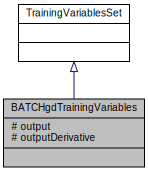
\includegraphics[width=220pt]{class_b_a_t_c_hgd_training_variables__inherit__graph}
\end{center}
\end{figure}


Collaboration diagram for BATCHgdTrainingVariables:\nopagebreak
\begin{figure}[H]
\begin{center}
\leavevmode
\includegraphics[width=220pt]{class_b_a_t_c_hgd_training_variables__coll__graph}
\end{center}
\end{figure}
\subsection*{Protected Attributes}
\begin{DoxyCompactItemize}
\item 
double \hyperlink{class_b_a_t_c_hgd_training_variables_a7cb844dac6feb79b1976cbd8db80c049}{output}
\item 
double \hyperlink{class_b_a_t_c_hgd_training_variables_ab02f509ad94944717a946c2cb16997fd}{outputDerivative}
\end{DoxyCompactItemize}


\subsection{Detailed Description}
class \hyperlink{class_b_a_t_c_hgd_training_variables}{BATCHgdTrainingVariables} -\/ 

Definition at line 5 of file BATCHgdTrainingVariables.h.



\subsection{Member Data Documentation}
\hypertarget{class_b_a_t_c_hgd_training_variables_a7cb844dac6feb79b1976cbd8db80c049}{
\index{BATCHgdTrainingVariables@{BATCHgdTrainingVariables}!output@{output}}
\index{output@{output}!BATCHgdTrainingVariables@{BATCHgdTrainingVariables}}
\subsubsection[{output}]{\setlength{\rightskip}{0pt plus 5cm}double {\bf BATCHgdTrainingVariables::output}\hspace{0.3cm}{\ttfamily  \mbox{[}protected\mbox{]}}}}
\label{class_b_a_t_c_hgd_training_variables_a7cb844dac6feb79b1976cbd8db80c049}


Definition at line 8 of file BATCHgdTrainingVariables.h.

\hypertarget{class_b_a_t_c_hgd_training_variables_ab02f509ad94944717a946c2cb16997fd}{
\index{BATCHgdTrainingVariables@{BATCHgdTrainingVariables}!outputDerivative@{outputDerivative}}
\index{outputDerivative@{outputDerivative}!BATCHgdTrainingVariables@{BATCHgdTrainingVariables}}
\subsubsection[{outputDerivative}]{\setlength{\rightskip}{0pt plus 5cm}double {\bf BATCHgdTrainingVariables::outputDerivative}\hspace{0.3cm}{\ttfamily  \mbox{[}protected\mbox{]}}}}
\label{class_b_a_t_c_hgd_training_variables_ab02f509ad94944717a946c2cb16997fd}


Definition at line 9 of file BATCHgdTrainingVariables.h.



The documentation for this class was generated from the following file:\begin{DoxyCompactItemize}
\item 
pkg/AMORE/src/dia/\hyperlink{_b_a_t_c_hgd_training_variables_8h}{BATCHgdTrainingVariables.h}\end{DoxyCompactItemize}

\hypertarget{class_b_a_t_c_hgdwm_training_variables}{
\section{BATCHgdwmTrainingVariables Class Reference}
\label{class_b_a_t_c_hgdwm_training_variables}\index{BATCHgdwmTrainingVariables@{BATCHgdwmTrainingVariables}}
}


class \hyperlink{class_b_a_t_c_hgdwm_training_variables}{BATCHgdwmTrainingVariables} -\/  




{\ttfamily \#include $<$BATCHgdwmTrainingVariables.h$>$}



Inheritance diagram for BATCHgdwmTrainingVariables:\nopagebreak
\begin{figure}[H]
\begin{center}
\leavevmode
\includegraphics[width=238pt]{class_b_a_t_c_hgdwm_training_variables__inherit__graph}
\end{center}
\end{figure}


Collaboration diagram for BATCHgdwmTrainingVariables:\nopagebreak
\begin{figure}[H]
\begin{center}
\leavevmode
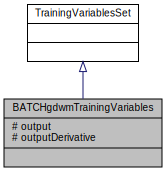
\includegraphics[width=238pt]{class_b_a_t_c_hgdwm_training_variables__coll__graph}
\end{center}
\end{figure}
\subsection*{Protected Attributes}
\begin{DoxyCompactItemize}
\item 
double \hyperlink{class_b_a_t_c_hgdwm_training_variables_a3f1f3635969b2d72bd117eda7afefada}{output}
\item 
double \hyperlink{class_b_a_t_c_hgdwm_training_variables_a985738d0f21b931cbb837ee3fa65dfcd}{outputDerivative}
\end{DoxyCompactItemize}


\subsection{Detailed Description}
class \hyperlink{class_b_a_t_c_hgdwm_training_variables}{BATCHgdwmTrainingVariables} -\/ 

Definition at line 5 of file BATCHgdwmTrainingVariables.h.



\subsection{Member Data Documentation}
\hypertarget{class_b_a_t_c_hgdwm_training_variables_a3f1f3635969b2d72bd117eda7afefada}{
\index{BATCHgdwmTrainingVariables@{BATCHgdwmTrainingVariables}!output@{output}}
\index{output@{output}!BATCHgdwmTrainingVariables@{BATCHgdwmTrainingVariables}}
\subsubsection[{output}]{\setlength{\rightskip}{0pt plus 5cm}double {\bf BATCHgdwmTrainingVariables::output}\hspace{0.3cm}{\ttfamily  \mbox{[}protected\mbox{]}}}}
\label{class_b_a_t_c_hgdwm_training_variables_a3f1f3635969b2d72bd117eda7afefada}


Definition at line 8 of file BATCHgdwmTrainingVariables.h.

\hypertarget{class_b_a_t_c_hgdwm_training_variables_a985738d0f21b931cbb837ee3fa65dfcd}{
\index{BATCHgdwmTrainingVariables@{BATCHgdwmTrainingVariables}!outputDerivative@{outputDerivative}}
\index{outputDerivative@{outputDerivative}!BATCHgdwmTrainingVariables@{BATCHgdwmTrainingVariables}}
\subsubsection[{outputDerivative}]{\setlength{\rightskip}{0pt plus 5cm}double {\bf BATCHgdwmTrainingVariables::outputDerivative}\hspace{0.3cm}{\ttfamily  \mbox{[}protected\mbox{]}}}}
\label{class_b_a_t_c_hgdwm_training_variables_a985738d0f21b931cbb837ee3fa65dfcd}


Definition at line 9 of file BATCHgdwmTrainingVariables.h.



The documentation for this class was generated from the following file:\begin{DoxyCompactItemize}
\item 
pkg/AMORE/src/dia/\hyperlink{_b_a_t_c_hgdwm_training_variables_8h}{BATCHgdwmTrainingVariables.h}\end{DoxyCompactItemize}

\hypertarget{struct_compare_id}{
\section{CompareId Struct Reference}
\label{struct_compare_id}\index{CompareId@{CompareId}}
}
\subsection*{Public Member Functions}
\begin{DoxyCompactItemize}
\item 
bool \hyperlink{struct_compare_id_a470bef628ec23bbdbd8f3bb103e60814}{operator()} (const \hyperlink{_a_m_o_r_e_8h_ae7d05d5880745e8a588e1efd62c81f32}{ConSharedPtr} a, const \hyperlink{_a_m_o_r_e_8h_ae7d05d5880745e8a588e1efd62c81f32}{ConSharedPtr} b)
\item 
bool \hyperlink{struct_compare_id_a2342f4d0e9448a2af26314e7f8ff94ec}{operator()} (const \hyperlink{_a_m_o_r_e_8h_ae7d05d5880745e8a588e1efd62c81f32}{ConSharedPtr} a, const int b)
\item 
bool \hyperlink{struct_compare_id_a43e46a0d30eb25672a449b7365bb6f31}{operator()} (const int a, const \hyperlink{_a_m_o_r_e_8h_ae7d05d5880745e8a588e1efd62c81f32}{ConSharedPtr} b)
\item 
bool \hyperlink{struct_compare_id_a1310378d3e8c8a9e4c74f6f0ac239c05}{operator()} (const int a, const int b)
\end{DoxyCompactItemize}


\subsection{Detailed Description}


Definition at line 359 of file vecCon.cpp.



\subsection{Member Function Documentation}
\hypertarget{struct_compare_id_a470bef628ec23bbdbd8f3bb103e60814}{
\index{CompareId@{CompareId}!operator()@{operator()}}
\index{operator()@{operator()}!CompareId@{CompareId}}
\subsubsection[{operator()}]{\setlength{\rightskip}{0pt plus 5cm}bool CompareId::operator() (
\begin{DoxyParamCaption}
\item[{const {\bf ConSharedPtr}}]{a, }
\item[{const {\bf ConSharedPtr}}]{b}
\end{DoxyParamCaption}
)\hspace{0.3cm}{\ttfamily  \mbox{[}inline\mbox{]}}}}
\label{struct_compare_id_a470bef628ec23bbdbd8f3bb103e60814}


Definition at line 361 of file vecCon.cpp.


\begin{DoxyCode}
                                                                    {
        return a->getFromId() < b->getFromId();
    };
\end{DoxyCode}
\hypertarget{struct_compare_id_a1310378d3e8c8a9e4c74f6f0ac239c05}{
\index{CompareId@{CompareId}!operator()@{operator()}}
\index{operator()@{operator()}!CompareId@{CompareId}}
\subsubsection[{operator()}]{\setlength{\rightskip}{0pt plus 5cm}bool CompareId::operator() (
\begin{DoxyParamCaption}
\item[{const int}]{a, }
\item[{const int}]{b}
\end{DoxyParamCaption}
)\hspace{0.3cm}{\ttfamily  \mbox{[}inline\mbox{]}}}}
\label{struct_compare_id_a1310378d3e8c8a9e4c74f6f0ac239c05}


Definition at line 373 of file vecCon.cpp.


\begin{DoxyCode}
                                                  {
           return a < b;
       };
\end{DoxyCode}
\hypertarget{struct_compare_id_a43e46a0d30eb25672a449b7365bb6f31}{
\index{CompareId@{CompareId}!operator()@{operator()}}
\index{operator()@{operator()}!CompareId@{CompareId}}
\subsubsection[{operator()}]{\setlength{\rightskip}{0pt plus 5cm}bool CompareId::operator() (
\begin{DoxyParamCaption}
\item[{const int}]{a, }
\item[{const {\bf ConSharedPtr}}]{b}
\end{DoxyParamCaption}
)\hspace{0.3cm}{\ttfamily  \mbox{[}inline\mbox{]}}}}
\label{struct_compare_id_a43e46a0d30eb25672a449b7365bb6f31}


Definition at line 369 of file vecCon.cpp.


\begin{DoxyCode}
                                                           {
           return a < b->getFromId();
       };
\end{DoxyCode}
\hypertarget{struct_compare_id_a2342f4d0e9448a2af26314e7f8ff94ec}{
\index{CompareId@{CompareId}!operator()@{operator()}}
\index{operator()@{operator()}!CompareId@{CompareId}}
\subsubsection[{operator()}]{\setlength{\rightskip}{0pt plus 5cm}bool CompareId::operator() (
\begin{DoxyParamCaption}
\item[{const {\bf ConSharedPtr}}]{a, }
\item[{const int}]{b}
\end{DoxyParamCaption}
)\hspace{0.3cm}{\ttfamily  \mbox{[}inline\mbox{]}}}}
\label{struct_compare_id_a2342f4d0e9448a2af26314e7f8ff94ec}


Definition at line 365 of file vecCon.cpp.


\begin{DoxyCode}
                                                           {
           return a->getFromId() < b  ;
       };
\end{DoxyCode}


The documentation for this struct was generated from the following file:\begin{DoxyCompactItemize}
\item 
pkg/AMORE/src/\hyperlink{vec_con_8cpp}{vecCon.cpp}\end{DoxyCompactItemize}

\hypertarget{class_con}{
\section{Con Class Reference}
\label{class_con}\index{Con@{Con}}
}


class \hyperlink{class_con}{Con} -\/  




{\ttfamily \#include $<$Con.h$>$}

\subsection*{Public Member Functions}
\begin{DoxyCompactItemize}
\item 
\hyperlink{class_con_a7fab3ece0e894f44f31d10a21b1d49c7}{Con} (\hyperlink{class_neuron}{Neuron} \&neuron)
\begin{DoxyCompactList}\small\item\em Constructor. \end{DoxyCompactList}\item 
\hyperlink{class_con_ad0b1e0d1eefd2296b23a2cfea04fc559}{Con} (\hyperlink{class_neuron}{Neuron} \&neuron, double weight)
\begin{DoxyCompactList}\small\item\em Constructor. \end{DoxyCompactList}\item 
\hyperlink{_a_m_o_r_e_8h_abc871abb71cff6655b8172ee7240b8ef}{Handler} \hyperlink{class_con_aee0a0b6c5beff6e227f9ebf33af2d209}{Id} ()
\begin{DoxyCompactList}\small\item\em A getter of the Id of the \hyperlink{class_neuron}{Neuron} pointed by the from field. \end{DoxyCompactList}\item 
\hyperlink{class_neuron}{Neuron} \& \hyperlink{class_con_a2209567efd330a58825b5068a421afe1}{getNeuron} ()
\begin{DoxyCompactList}\small\item\em from field accessor. \end{DoxyCompactList}\item 
void \hyperlink{class_con_ae372f50a253a424376959fb6ee8f083b}{setNeuron} (\hyperlink{class_neuron}{Neuron} \&neuron)
\item 
double \hyperlink{class_con_a385c5bf6eb9e2ffc94c5b427c287ccb2}{getWeight} ()
\begin{DoxyCompactList}\small\item\em weight field accessor. \end{DoxyCompactList}\item 
void \hyperlink{class_con_acf3b130556e25414cd525d469b275239}{setWeight} (double weight)
\item 
void \hyperlink{class_con_a6fac8dbf2a320d6fb674295a9c900a8a}{show} ()
\begin{DoxyCompactList}\small\item\em Pretty print of the \hyperlink{class_con}{Con} information. \end{DoxyCompactList}\item 
bool \hyperlink{class_con_af5f836a7b0988b3d9113589b2959d5e6}{validate} ()
\begin{DoxyCompactList}\small\item\em Object validator. \end{DoxyCompactList}\end{DoxyCompactItemize}
\subsection*{Private Attributes}
\begin{DoxyCompactItemize}
\item 
\hyperlink{_a_m_o_r_e_8h_ae4f8e0af6c35f16f9f1d3588d8915cf6}{NeuronRef} \hyperlink{class_con_aad857bd289343ecff2153acc852f34f0}{d\_\-neuron}
\item 
double \hyperlink{class_con_a41e043e0dfb126f3bdacbbd8caf33672}{d\_\-weight}
\end{DoxyCompactItemize}


\subsection{Detailed Description}
class \hyperlink{class_con}{Con} -\/ 

Definition at line 3 of file Con.h.



\subsection{Constructor \& Destructor Documentation}
\hypertarget{class_con_a7fab3ece0e894f44f31d10a21b1d49c7}{
\index{Con@{Con}!Con@{Con}}
\index{Con@{Con}!Con@{Con}}
\subsubsection[{Con}]{\setlength{\rightskip}{0pt plus 5cm}Con::Con (
\begin{DoxyParamCaption}
\item[{{\bf Neuron} \&}]{neuron}
\end{DoxyParamCaption}
)}}
\label{class_con_a7fab3ece0e894f44f31d10a21b1d49c7}


Constructor. 



Definition at line 19 of file Con.cpp.


\begin{DoxyCode}
                       :
  d_neuron( boost::ref(neuron) ), d_weight(0)
{
}
\end{DoxyCode}
\hypertarget{class_con_ad0b1e0d1eefd2296b23a2cfea04fc559}{
\index{Con@{Con}!Con@{Con}}
\index{Con@{Con}!Con@{Con}}
\subsubsection[{Con}]{\setlength{\rightskip}{0pt plus 5cm}Con::Con (
\begin{DoxyParamCaption}
\item[{{\bf Neuron} \&}]{neuron, }
\item[{double}]{weight}
\end{DoxyParamCaption}
)}}
\label{class_con_ad0b1e0d1eefd2296b23a2cfea04fc559}


Constructor. 



Definition at line 30 of file Con.cpp.


\begin{DoxyCode}
                                      :
  d_neuron(boost::ref(neuron)), d_weight(weight)
{
}
\end{DoxyCode}


\subsection{Member Function Documentation}
\hypertarget{class_con_a2209567efd330a58825b5068a421afe1}{
\index{Con@{Con}!getNeuron@{getNeuron}}
\index{getNeuron@{getNeuron}!Con@{Con}}
\subsubsection[{getNeuron}]{\setlength{\rightskip}{0pt plus 5cm}{\bf Neuron} \& Con::getNeuron (
\begin{DoxyParamCaption}
{}
\end{DoxyParamCaption}
)}}
\label{class_con_a2209567efd330a58825b5068a421afe1}


from field accessor. 

This method allows access to the address stored in the private from field (a pointer to a \hyperlink{class_neuron}{Neuron} object).$\ast$ \begin{DoxyReturn}{Returns}
A pointer to the \hyperlink{class_neuron}{Neuron} object referred to by the from field.
\end{DoxyReturn}

\begin{DoxyCode}
        //================
        //Usage example:
        //================
        // Data set up
                        NeuronPtr ptShNeuron ( new Neuron(1) );         // Neuron
       Id is set 1
                        ConPtr ptShCon( new Con(ptShNeuron) );          // from p
      oints to ptShNeuron and weight is set to 0
        // Test
                        ptShNeuron = ptShCon->getFrom() ;
                        int result = ptShNeuron->getId();

        // Now, result is equal to 1.
\end{DoxyCode}


\begin{DoxySeeAlso}{See also}
getId and the unit test files, e.g., runit.Cpp.Con.R, for further examples. 
\end{DoxySeeAlso}


Definition at line 56 of file Con.cpp.



References d\_\-neuron.


\begin{DoxyCode}
{
  return d_neuron;
}
\end{DoxyCode}
\hypertarget{class_con_a385c5bf6eb9e2ffc94c5b427c287ccb2}{
\index{Con@{Con}!getWeight@{getWeight}}
\index{getWeight@{getWeight}!Con@{Con}}
\subsubsection[{getWeight}]{\setlength{\rightskip}{0pt plus 5cm}double Con::getWeight (
\begin{DoxyParamCaption}
{}
\end{DoxyParamCaption}
)}}
\label{class_con_a385c5bf6eb9e2ffc94c5b427c287ccb2}


weight field accessor. 

This method allows access to the value stored in the private field weight \begin{DoxyReturn}{Returns}
The value of weight (double)
\end{DoxyReturn}

\begin{DoxyCode}
  //================
  //Usage example:
  //================
  // Data set up
                        std::vector<double> result;
                        NeuronPtr ptShNeuron ( new Neuron(16) );                /
      / Neuron Id is set to 16
                        ConPtr ptShCon( new Con(ptShNeuron, 12.4) );  // from poi
      nts to ptShNeuron and weight is set to 12.4
        // Test
                        result.push_back( ptShCon->getWeight() );
                        ptShCon->setWeight(2.2);
                        result.push_back( ptShCon->getWeight() );

        // Now, result is a numeric vector that contains the values 12.4 and 2.2 
      .
\end{DoxyCode}


\begin{DoxySeeAlso}{See also}
\hyperlink{class_con_acf3b130556e25414cd525d469b275239}{setWeight} and the unit test files, e.g., runit.Cpp.Con.R, for further examples. 
\end{DoxySeeAlso}


Definition at line 116 of file Con.cpp.



References d\_\-weight.



Referenced by show(), and validate().


\begin{DoxyCode}
{
  return d_weight;
}
\end{DoxyCode}


Here is the caller graph for this function:
\nopagebreak
\begin{figure}[H]
\begin{center}
\leavevmode
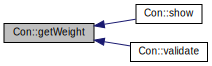
\includegraphics[width=284pt]{class_con_a385c5bf6eb9e2ffc94c5b427c287ccb2_icgraph}
\end{center}
\end{figure}


\hypertarget{class_con_aee0a0b6c5beff6e227f9ebf33af2d209}{
\index{Con@{Con}!Id@{Id}}
\index{Id@{Id}!Con@{Con}}
\subsubsection[{Id}]{\setlength{\rightskip}{0pt plus 5cm}int Con::Id (
\begin{DoxyParamCaption}
{}
\end{DoxyParamCaption}
)}}
\label{class_con_aee0a0b6c5beff6e227f9ebf33af2d209}


A getter of the Id of the \hyperlink{class_neuron}{Neuron} pointed by the from field. 

This method gets the Id of the \hyperlink{class_neuron}{Neuron} referred to by the from field \begin{DoxyReturn}{Returns}
The value of the Id (an integer).
\end{DoxyReturn}

\begin{DoxyCode}
      //================
      //Usage example:
      //================
      // Data set up
                      NeuronPtr ptShNeuron ( new Neuron(16) );        // Neuron I
      d is set to 16
                      ConPtr ptShCon( new Con(ptShNeuron) );          // from poi
      nts to ptShNeuron and weight is set to 0
      // Test
                      int result = ptShCon->getId();

      // Now, result is equal to 16.
\end{DoxyCode}


\begin{DoxySeeAlso}{See also}
getFrom, setFrom and the unit test files, e.g., runit.Cpp.Con.R, for further examples. 
\end{DoxySeeAlso}


Definition at line 88 of file Con.cpp.



References d\_\-neuron.



Referenced by show(), and validate().


\begin{DoxyCode}
{
  return d_neuron.get().getId();
}
\end{DoxyCode}


Here is the caller graph for this function:
\nopagebreak
\begin{figure}[H]
\begin{center}
\leavevmode
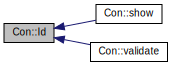
\includegraphics[width=244pt]{class_con_aee0a0b6c5beff6e227f9ebf33af2d209_icgraph}
\end{center}
\end{figure}


\hypertarget{class_con_ae372f50a253a424376959fb6ee8f083b}{
\index{Con@{Con}!setNeuron@{setNeuron}}
\index{setNeuron@{setNeuron}!Con@{Con}}
\subsubsection[{setNeuron}]{\setlength{\rightskip}{0pt plus 5cm}void Con::setNeuron (
\begin{DoxyParamCaption}
\item[{{\bf Neuron} \&}]{neuron}
\end{DoxyParamCaption}
)}}
\label{class_con_ae372f50a253a424376959fb6ee8f083b}


Definition at line 63 of file Con.cpp.



References d\_\-neuron.


\begin{DoxyCode}
{
  d_neuron=boost::ref(neuron);
}
\end{DoxyCode}
\hypertarget{class_con_acf3b130556e25414cd525d469b275239}{
\index{Con@{Con}!setWeight@{setWeight}}
\index{setWeight@{setWeight}!Con@{Con}}
\subsubsection[{setWeight}]{\setlength{\rightskip}{0pt plus 5cm}void Con::setWeight (
\begin{DoxyParamCaption}
\item[{double}]{weight}
\end{DoxyParamCaption}
)}}
\label{class_con_acf3b130556e25414cd525d469b275239}


Definition at line 123 of file Con.cpp.



References d\_\-weight.


\begin{DoxyCode}
{
  d_weight=weight;
}
\end{DoxyCode}
\hypertarget{class_con_a6fac8dbf2a320d6fb674295a9c900a8a}{
\index{Con@{Con}!show@{show}}
\index{show@{show}!Con@{Con}}
\subsubsection[{show}]{\setlength{\rightskip}{0pt plus 5cm}void Con::show (
\begin{DoxyParamCaption}
{}
\end{DoxyParamCaption}
)}}
\label{class_con_a6fac8dbf2a320d6fb674295a9c900a8a}


Pretty print of the \hyperlink{class_con}{Con} information. 

This method outputs in the R terminal the contents of the \hyperlink{class_con}{Con} fields. \begin{DoxyReturn}{Returns}
true in case everything works without throwing an exception 
\end{DoxyReturn}
\begin{DoxySeeAlso}{See also}
\hyperlink{class_con_acf3b130556e25414cd525d469b275239}{setWeight} and the unit test files, e.g., runit.Cpp.Con.R, for usage examples. 
\end{DoxySeeAlso}


Definition at line 135 of file Con.cpp.



References getWeight(), and Id().


\begin{DoxyCode}
{
  int id = Id();
  if (id == NA_INTEGER)
    {
      Rprintf("From: NA\t Invalid Connection \n");
    }
  else
    {
      Rprintf("From:\t %d \t Weight= \t %lf \n", id , getWeight() );
    }
}
\end{DoxyCode}


Here is the call graph for this function:
\nopagebreak
\begin{figure}[H]
\begin{center}
\leavevmode
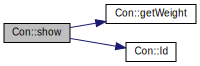
\includegraphics[width=272pt]{class_con_a6fac8dbf2a320d6fb674295a9c900a8a_cgraph}
\end{center}
\end{figure}


\hypertarget{class_con_af5f836a7b0988b3d9113589b2959d5e6}{
\index{Con@{Con}!validate@{validate}}
\index{validate@{validate}!Con@{Con}}
\subsubsection[{validate}]{\setlength{\rightskip}{0pt plus 5cm}bool Con::validate (
\begin{DoxyParamCaption}
{}
\end{DoxyParamCaption}
)}}
\label{class_con_af5f836a7b0988b3d9113589b2959d5e6}


Object validator. 

This method checks the object for internal coherence. A try / catch mechanism exits normal execution and returns control to the R terminal in case the contents of the \hyperlink{class_con}{Con} object are identified as corrupted. \begin{DoxyReturn}{Returns}
true in case the checks are Ok. 
\end{DoxyReturn}

\begin{DoxyExceptions}{Exceptions}
{\em An} & std::range error if weight or from are not finite. \\
\hline
\end{DoxyExceptions}


Definition at line 155 of file Con.cpp.



References getWeight(), and Id().


\begin{DoxyCode}
{
  BEGIN_RCPP
  if (! R_FINITE(getWeight()) ) throw std::range_error("weight is not finite.");
  if (Id() == NA_INTEGER)
    throw std::range_error("fromId is not finite.");
  return (true);
END_RCPP}
\end{DoxyCode}


Here is the call graph for this function:\nopagebreak
\begin{figure}[H]
\begin{center}
\leavevmode
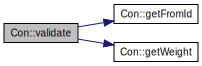
\includegraphics[width=284pt]{class_con_af5f836a7b0988b3d9113589b2959d5e6_cgraph}
\end{center}
\end{figure}




\subsection{Member Data Documentation}
\hypertarget{class_con_aad857bd289343ecff2153acc852f34f0}{
\index{Con@{Con}!d\_\-neuron@{d\_\-neuron}}
\index{d\_\-neuron@{d\_\-neuron}!Con@{Con}}
\subsubsection[{d\_\-neuron}]{\setlength{\rightskip}{0pt plus 5cm}{\bf NeuronRef} {\bf Con::d\_\-neuron}\hspace{0.3cm}{\ttfamily  \mbox{[}private\mbox{]}}}}
\label{class_con_aad857bd289343ecff2153acc852f34f0}


Definition at line 6 of file Con.h.



Referenced by getNeuron(), Id(), and setNeuron().

\hypertarget{class_con_a41e043e0dfb126f3bdacbbd8caf33672}{
\index{Con@{Con}!d\_\-weight@{d\_\-weight}}
\index{d\_\-weight@{d\_\-weight}!Con@{Con}}
\subsubsection[{d\_\-weight}]{\setlength{\rightskip}{0pt plus 5cm}double {\bf Con::d\_\-weight}\hspace{0.3cm}{\ttfamily  \mbox{[}private\mbox{]}}}}
\label{class_con_a41e043e0dfb126f3bdacbbd8caf33672}


Definition at line 7 of file Con.h.



Referenced by getWeight(), and setWeight().



The documentation for this class was generated from the following files:\begin{DoxyCompactItemize}
\item 
pkg/AMORE/src/dia/\hyperlink{_con_8h}{Con.h}\item 
pkg/AMORE/src/\hyperlink{_con_8cpp}{Con.cpp}\end{DoxyCompactItemize}

\hypertarget{class_con_container}{
\section{ConContainer Class Reference}
\label{class_con_container}\index{ConContainer@{ConContainer}}
}


A vector of connections.  




{\ttfamily \#include $<$ConContainer.h$>$}



Inheritance diagram for ConContainer:\nopagebreak
\begin{figure}[H]
\begin{center}
\leavevmode
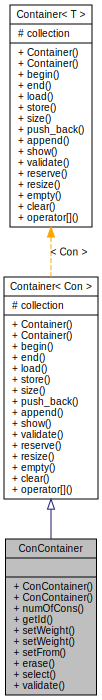
\includegraphics[height=600pt]{class_con_container__inherit__graph}
\end{center}
\end{figure}


Collaboration diagram for ConContainer:\nopagebreak
\begin{figure}[H]
\begin{center}
\leavevmode
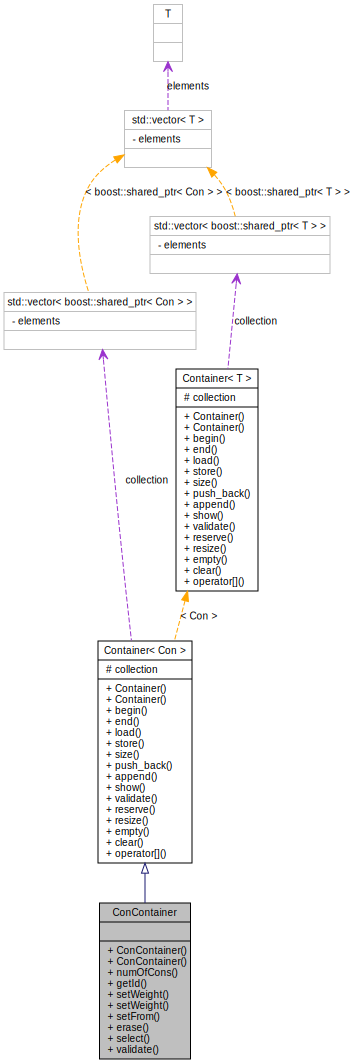
\includegraphics[height=600pt]{class_con_container__coll__graph}
\end{center}
\end{figure}
\subsection*{Public Types}
\begin{DoxyCompactItemize}
\item 
typedef std::vector$<$ boost::shared\_\-ptr$<$ \hyperlink{class_con}{Con} $>$ $>$::\hyperlink{class_con_container_a5dc8aab66a22fc25b7e700b51265b577}{iterator} \hyperlink{class_con_container_a5dc8aab66a22fc25b7e700b51265b577}{iterator}
\item 
typedef std::vector$<$ boost::shared\_\-ptr$<$ \hyperlink{class_con}{Con} $>$ $>$::\hyperlink{class_con_container_ac314ee4e351b3a5f595cd1de74fb3b5e}{const\_\-iterator} \hyperlink{class_con_container_ac314ee4e351b3a5f595cd1de74fb3b5e}{const\_\-iterator}
\item 
typedef boost::shared\_\-ptr$<$ \hyperlink{class_con}{Con} $>$ \hyperlink{class_con_container_a08881a149e3a285eba67a4c8cff92a9e}{value\_\-type}
\item 
typedef \hyperlink{class_con_container_a08881a149e3a285eba67a4c8cff92a9e}{value\_\-type} const \& \hyperlink{class_con_container_ac644eca2f5ee432a6070fd1d397b3741}{const\_\-reference}
\end{DoxyCompactItemize}
\subsection*{Public Member Functions}
\begin{DoxyCompactItemize}
\item 
\hyperlink{class_con_container_aec4578b20ba3509e450bfbc9851d3393}{ConContainer} ()
\item 
\hyperlink{class_con_container_a69e83fdaf298e23758fe7ead2fe488b9}{ConContainer} (std::vector$<$ \hyperlink{_a_m_o_r_e_8h_a169bb8e5f26ce70bf2b10dec2fb5ee50}{ConPtr} $>$ \hyperlink{class_container_a6cc12233bceb7d72709320d2c57e3398}{collection})
\item 
int \hyperlink{class_con_container_a8895e2c10e223e9950028f595588b9fe}{numOfCons} ()
\begin{DoxyCompactList}\small\item\em Size of the \hyperlink{class_con_container}{ConContainer} object. \end{DoxyCompactList}\item 
std::vector$<$ int $>$ \hyperlink{class_con_container_a387ac09ab154d21c5ad597d32b32dbc2}{getId} ()
\begin{DoxyCompactList}\small\item\em Getter of the Id values of the vector of Cons. \end{DoxyCompactList}\item 
bool \hyperlink{class_con_container_a36dc3c4d86e63eda0a1e9ba17179c0f9}{setWeight} (std::vector$<$ double $>$ nWeights)
\begin{DoxyCompactList}\small\item\em Setter of the weight field of the \hyperlink{class_con}{Con} objects related to \hyperlink{class_con_container}{ConContainer}. \end{DoxyCompactList}\item 
bool \hyperlink{class_con_container_a2b9d4d12f0e5948b37ccd23445eaef7c}{setWeight} (std::vector$<$ double $>$ nWeights, std::vector$<$ int $>$ nIds)
\begin{DoxyCompactList}\small\item\em Setter of the weights of the specified elements from the \hyperlink{class_con_container}{ConContainer} object. \end{DoxyCompactList}\item 
bool \hyperlink{class_con_container_aa7f1bbd910afe9c4241e8bd4d5fbc497}{setFrom} (\hyperlink{class_neuron_container}{NeuronContainer} neuronContainer)
\begin{DoxyCompactList}\small\item\em Setter of the from fields of the \hyperlink{class_con}{Con} objects related to \hyperlink{class_con_container}{ConContainer}. \end{DoxyCompactList}\item 
void \hyperlink{class_con_container_a9665acde2f526ae4207b919c90615fe5}{erase} (std::vector$<$ int $>$ nIds)
\begin{DoxyCompactList}\small\item\em Erase the specified elements from the vecCom object. \end{DoxyCompactList}\item 
ConContainerPtr \hyperlink{class_con_container_a7fb490683bd4733cae3c6428bad9328c}{select} (std::vector$<$ int $>$ nIds)
\begin{DoxyCompactList}\small\item\em Selects the specified elements from the vecCom object. \end{DoxyCompactList}\item 
bool \hyperlink{class_con_container_aac12a3d3604db9ff715503816109470c}{validate} ()
\begin{DoxyCompactList}\small\item\em Object validator. \end{DoxyCompactList}\end{DoxyCompactItemize}


\subsection{Detailed Description}
A vector of connections. 

The \hyperlink{class_con_container}{ConContainer} class provides a simple class for a vector of connections. It's named after the R equivalent Reference Class. 

Definition at line 16 of file ConContainer.h.



\subsection{Member Typedef Documentation}
\hypertarget{class_con_container_ac314ee4e351b3a5f595cd1de74fb3b5e}{
\index{ConContainer@{ConContainer}!const\_\-iterator@{const\_\-iterator}}
\index{const\_\-iterator@{const\_\-iterator}!ConContainer@{ConContainer}}
\subsubsection[{const\_\-iterator}]{\setlength{\rightskip}{0pt plus 5cm}typedef std::vector$<$boost::shared\_\-ptr$<${\bf Con}$>$ $>$::{\bf const\_\-iterator} {\bf ConContainer::const\_\-iterator}}}
\label{class_con_container_ac314ee4e351b3a5f595cd1de74fb3b5e}


Reimplemented from \hyperlink{class_container_a5eabadaffdd508cb623c955eb0af1518}{Container$<$ Con $>$}.



Definition at line 23 of file ConContainer.h.

\hypertarget{class_con_container_ac644eca2f5ee432a6070fd1d397b3741}{
\index{ConContainer@{ConContainer}!const\_\-reference@{const\_\-reference}}
\index{const\_\-reference@{const\_\-reference}!ConContainer@{ConContainer}}
\subsubsection[{const\_\-reference}]{\setlength{\rightskip}{0pt plus 5cm}typedef {\bf value\_\-type} const\& {\bf ConContainer::const\_\-reference}}}
\label{class_con_container_ac644eca2f5ee432a6070fd1d397b3741}


Reimplemented from \hyperlink{class_container_a8dd7ae9d0687e11d873f98206e961ac1}{Container$<$ Con $>$}.



Definition at line 27 of file ConContainer.h.

\hypertarget{class_con_container_a5dc8aab66a22fc25b7e700b51265b577}{
\index{ConContainer@{ConContainer}!iterator@{iterator}}
\index{iterator@{iterator}!ConContainer@{ConContainer}}
\subsubsection[{iterator}]{\setlength{\rightskip}{0pt plus 5cm}typedef std::vector$<$boost::shared\_\-ptr$<${\bf Con}$>$ $>$::{\bf iterator} {\bf ConContainer::iterator}}}
\label{class_con_container_a5dc8aab66a22fc25b7e700b51265b577}


Reimplemented from \hyperlink{class_container_afe880028d8304353129f47cd1d28c20a}{Container$<$ Con $>$}.



Definition at line 21 of file ConContainer.h.

\hypertarget{class_con_container_a08881a149e3a285eba67a4c8cff92a9e}{
\index{ConContainer@{ConContainer}!value\_\-type@{value\_\-type}}
\index{value\_\-type@{value\_\-type}!ConContainer@{ConContainer}}
\subsubsection[{value\_\-type}]{\setlength{\rightskip}{0pt plus 5cm}typedef boost::shared\_\-ptr$<${\bf Con}$>$ {\bf ConContainer::value\_\-type}}}
\label{class_con_container_a08881a149e3a285eba67a4c8cff92a9e}


Reimplemented from \hyperlink{class_container_aa44714b9a736d2cfd2e01a87ad1c001b}{Container$<$ Con $>$}.



Definition at line 25 of file ConContainer.h.



\subsection{Constructor \& Destructor Documentation}
\hypertarget{class_con_container_aec4578b20ba3509e450bfbc9851d3393}{
\index{ConContainer@{ConContainer}!ConContainer@{ConContainer}}
\index{ConContainer@{ConContainer}!ConContainer@{ConContainer}}
\subsubsection[{ConContainer}]{\setlength{\rightskip}{0pt plus 5cm}ConContainer::ConContainer (
\begin{DoxyParamCaption}
{}
\end{DoxyParamCaption}
)}}
\label{class_con_container_aec4578b20ba3509e450bfbc9851d3393}


Definition at line 8 of file ConContainer.cpp.


\begin{DoxyCode}
{
}
\end{DoxyCode}
\hypertarget{class_con_container_a69e83fdaf298e23758fe7ead2fe488b9}{
\index{ConContainer@{ConContainer}!ConContainer@{ConContainer}}
\index{ConContainer@{ConContainer}!ConContainer@{ConContainer}}
\subsubsection[{ConContainer}]{\setlength{\rightskip}{0pt plus 5cm}ConContainer::ConContainer (
\begin{DoxyParamCaption}
\item[{std::vector$<$ {\bf ConPtr} $>$}]{collection}
\end{DoxyParamCaption}
)}}
\label{class_con_container_a69e83fdaf298e23758fe7ead2fe488b9}


Definition at line 12 of file ConContainer.cpp.


\begin{DoxyCode}
                                                       :
  Container<Con> (collection) // Call to Base constructor
{
}
\end{DoxyCode}


\subsection{Member Function Documentation}
\hypertarget{class_con_container_a9665acde2f526ae4207b919c90615fe5}{
\index{ConContainer@{ConContainer}!erase@{erase}}
\index{erase@{erase}!ConContainer@{ConContainer}}
\subsubsection[{erase}]{\setlength{\rightskip}{0pt plus 5cm}void ConContainer::erase (
\begin{DoxyParamCaption}
\item[{std::vector$<$ int $>$}]{nIds}
\end{DoxyParamCaption}
)}}
\label{class_con_container_a9665acde2f526ae4207b919c90615fe5}


Erase the specified elements from the vecCom object. 

Provides a convenient way of removing some \hyperlink{class_con}{Con} objects from the collection field of the \hyperlink{class_con_container}{ConContainer} object.


\begin{DoxyParams}{Parameters}
{\em vFrom} & An std::vector$<$int$>$ with the Ids of the connections to remove.\\
\hline
\end{DoxyParams}

\begin{DoxyCode}
        //================
        //Usage example:
        //================

        // Data set up
                        std::vector<int> result;
                        std::vector<NeuronPtr> neuronContainer;
                        ConContainerPtr conContainerPtr( new ConContainer() );
                        ConContainerPtr vErased;
                        ConPtr  ptC;
                        NeuronPtr ptN;
                        int ids[]= {11, 10, 9, 3, 4, 5, 6, 7, 8, 2, 1};
                        std::vector<double> nWeights;
                        nWeights.push_back(11.32);
                        nWeights.push_back(1.26);
                        nWeights.push_back(2.14);
                        nWeights.push_back(3.16);
                        nWeights.push_back(4.14);
                        nWeights.push_back(5.19);
                        nWeights.push_back(6.18);
                        nWeights.push_back(7.16);
                        nWeights.push_back(8.14);
                        nWeights.push_back(9.12);
                        nWeights.push_back(10.31);

                        for (int i=0; i<nWeights.size() ; i++) {                                /
      / Let's create a vector with three neurons
                                ptN.reset( new Neuron( ids[i] ) );
                                neuronContainer.push_back(ptN);
                        }
                        conContainerPtr->buildAndAppend(neuronContainer, nWeights
      );

                        // Test

                        std::vector<int> toRemove;
                        toRemove.push_back(1);
                        toRemove.push_back(3);
                        toRemove.push_back(5);
                        toRemove.push_back(7);

                        conContainerPtr->erase(toRemove);
                        conContainerPtr->show();
                        result=conContainerPtr->getId();

                // The output at the R terminal would display :
                //
                // From:         2       Weight=         9.120000
                // From:         4       Weight=         4.140000
                // From:         6       Weight=         6.180000
                // From:         8       Weight=         8.140000
                // From:         9       Weight=         2.140000
                // From:         10  Weight=     1.260000
                // From:         11  Weight=     11.320000
\end{DoxyCode}


\begin{DoxySeeAlso}{See also}
\hyperlink{class_con_container_a7fb490683bd4733cae3c6428bad9328c}{select} and the unit test files, e.g. runit.Cpp.ConContainer.R, for further examples. 
\end{DoxySeeAlso}


Definition at line 450 of file ConContainer.cpp.



References Container$<$ Con $>$::begin(), Container$<$ Con $>$::end(), and Container$<$ Con $>$::resize().


\begin{DoxyCode}
{
  std::vector<ConPtr>::iterator itr;
  sort(begin(), end(), CompareId());
  sort(nIds.begin(), nIds.end());
  itr = set_difference(begin(), end(), nIds.begin(), nIds.end(), begin(),
      CompareId());
  resize(itr - begin());
}
\end{DoxyCode}


Here is the call graph for this function:\nopagebreak
\begin{figure}[H]
\begin{center}
\leavevmode
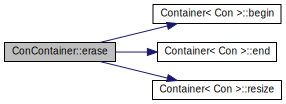
\includegraphics[width=358pt]{class_con_container_a9665acde2f526ae4207b919c90615fe5_cgraph}
\end{center}
\end{figure}


\hypertarget{class_con_container_a387ac09ab154d21c5ad597d32b32dbc2}{
\index{ConContainer@{ConContainer}!getId@{getId}}
\index{getId@{getId}!ConContainer@{ConContainer}}
\subsubsection[{getId}]{\setlength{\rightskip}{0pt plus 5cm}std::vector$<$ int $>$ ConContainer::getId (
\begin{DoxyParamCaption}
{}
\end{DoxyParamCaption}
)}}
\label{class_con_container_a387ac09ab154d21c5ad597d32b32dbc2}


Getter of the Id values of the vector of Cons. 

This function returns the Id's of the neurons referred to by the vector of Cons. \begin{DoxyReturn}{Returns}
An std::vector$<$int$>$ that contains the Ids
\end{DoxyReturn}

\begin{DoxyCode}
  //================
  //Usage example:
  //================
        // Data set up
                        Neuron N1, N2, N3;
                        ConContainer conContainer;
                        std::vector<int> result;

                        N1.setId(10);
                        N2.setId(20);
                        N3.setId(30);

                        ConPtr ptCon( new Con(&N1, 1.13) );     // Create new Con
       and initialize ptCon
                        conContainer.push_back(ptCon);                          /
      / push_back
                        ptCon.reset(  new Con(&N2, 2.22) );             // create
       new Con and assign to ptCon
                        conContainer.push_back(ptCon);                          /
      / push_back
                        ptCon.reset(  new Con(&N3, 3.33) );             // create
       new Con and assign to ptCon
                        conContainer.push_back(ptCon);                          /
      / push_back

        // Test
                        conContainer.show() ;
                        conContainer.validate();
                        result=conContainer.getId();

        // Now result is a vector that contains the values 10, 20 and 30.
\end{DoxyCode}


\begin{DoxySeeAlso}{See also}
getWeight and the unit test files, e.g. runit.Cpp.ConContainer.R, for further examples. 
\end{DoxySeeAlso}


Definition at line 93 of file ConContainer.cpp.



References numOfCons().



Referenced by validate().


\begin{DoxyCode}
{
  std::vector<int> result;
  result.reserve(numOfCons());
  foreach (ConPtr itr, *this)
    {
      result.push_back(itr->getId());
    }
  return result;
}
\end{DoxyCode}


Here is the call graph for this function:\nopagebreak
\begin{figure}[H]
\begin{center}
\leavevmode
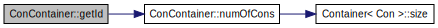
\includegraphics[width=400pt]{class_con_container_a387ac09ab154d21c5ad597d32b32dbc2_cgraph}
\end{center}
\end{figure}




Here is the caller graph for this function:\nopagebreak
\begin{figure}[H]
\begin{center}
\leavevmode
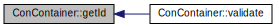
\includegraphics[width=348pt]{class_con_container_a387ac09ab154d21c5ad597d32b32dbc2_icgraph}
\end{center}
\end{figure}


\hypertarget{class_con_container_a8895e2c10e223e9950028f595588b9fe}{
\index{ConContainer@{ConContainer}!numOfCons@{numOfCons}}
\index{numOfCons@{numOfCons}!ConContainer@{ConContainer}}
\subsubsection[{numOfCons}]{\setlength{\rightskip}{0pt plus 5cm}int ConContainer::numOfCons (
\begin{DoxyParamCaption}
{}
\end{DoxyParamCaption}
)}}
\label{class_con_container_a8895e2c10e223e9950028f595588b9fe}


Size of the \hyperlink{class_con_container}{ConContainer} object. 

This function returns the size of the \hyperlink{class_con_container}{ConContainer} object, that is to say, the number of \hyperlink{class_con}{Con} objects it contains. \begin{DoxyReturn}{Returns}
The size of the vector
\end{DoxyReturn}

\begin{DoxyCode}
  //================
  //Usage example:
  //================
        // Data set up
                                std::vector<int> result;
                                std::vector<ConPtr> vcA, vcB;
                                ContainerNeuronPtr      neuronContainerPtr( new 
      Container<Neuron>() );
                                ConContainerPtr conContainerPtr( new 
      ConContainer() );
                                ConPtr  ptC;
                                NeuronPtr ptN;
                                int ids[]= {10, 20, 30};
                                double weights[] = {1.13, 2.22, 3.33 };
                                for (int i=0; i<=2 ; i++) {                             /
      / Let's create a vector with three neurons
                                        ptN.reset( new Neuron( ids[i] ) );
                                        neuronContainerPtr->push_back(ptN);
                                }
        // Test
                                for (int i=0; i<=2 ; i++) {                             /
      / and a vector with three connections
                                        result.push_back(conContainerPtr->numOfCo
      ns());          // Append numOfCons to result, create new Con and push_back into 
      conContainer
                                        ptC.reset( new Con( neuronContainerPtr->l
      oad().at(i), weights[i]) );
                                        conContainerPtr->push_back(ptC);
                                }

        // Now, result contains a numeric vector with values 0, 1, 2, and 3.
\end{DoxyCode}


\begin{DoxySeeAlso}{See also}
\hyperlink{class_container_a359f34bc418575b474184cbe3f33527e}{Container::size} (alias) 
\end{DoxySeeAlso}


Definition at line 52 of file ConContainer.cpp.



References Container$<$ Con $>$::size().



Referenced by getId().


\begin{DoxyCode}
{
  return size();
}
\end{DoxyCode}


Here is the call graph for this function:\nopagebreak
\begin{figure}[H]
\begin{center}
\leavevmode
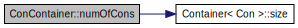
\includegraphics[width=376pt]{class_con_container_a8895e2c10e223e9950028f595588b9fe_cgraph}
\end{center}
\end{figure}




Here is the caller graph for this function:\nopagebreak
\begin{figure}[H]
\begin{center}
\leavevmode
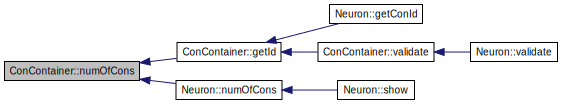
\includegraphics[width=400pt]{class_con_container_a8895e2c10e223e9950028f595588b9fe_icgraph}
\end{center}
\end{figure}


\hypertarget{class_con_container_a7fb490683bd4733cae3c6428bad9328c}{
\index{ConContainer@{ConContainer}!select@{select}}
\index{select@{select}!ConContainer@{ConContainer}}
\subsubsection[{select}]{\setlength{\rightskip}{0pt plus 5cm}ConContainerPtr ConContainer::select (
\begin{DoxyParamCaption}
\item[{std::vector$<$ int $>$}]{nIds}
\end{DoxyParamCaption}
)}}
\label{class_con_container_a7fb490683bd4733cae3c6428bad9328c}


Selects the specified elements from the vecCom object. 

Provides a convenient way of selecting some \hyperlink{class_con}{Con} objects from the collection field of the \hyperlink{class_con_container}{ConContainer} object.


\begin{DoxyParams}{Parameters}
{\em vFrom} & An std::vector$<$int$>$ with the Ids of the connections to select.\\
\hline
\end{DoxyParams}

\begin{DoxyCode}
        //================
        //Usage example:
        //================

        // Data set up
                std::vector<int> result;
                std::vector<NeuronPtr> neuronContainer;
                ConContainerPtr conContainerPtr( new ConContainer() );
                ConPtr  ptC;
                NeuronPtr ptN;
                int ids[]= {11, 10, 9, 3, 4, 5, 6, 7, 8, 2, 1};
                double weights[]={11.32, 1.26, 2.14, 3.16, 4.14, 5.19, 6.18, 7.16
      , 8.14, 9.12, 10.31};
                std::vector<double> nWeights;
                for (int i=0; i<11; i++) {
                        nWeights.push_back(weights[i]);
                }
                for (int i=0; i<nWeights.size() ; i++) {                                /
      / Let's create a vector with three neurons
                        ptN.reset( new Neuron( ids[i] ) );
                        neuronContainer.push_back(ptN);
                }
                conContainerPtr->buildAndAppend(neuronContainer, nWeights);
                // Test
                std::vector<int> toSelect;
                toSelect.push_back(1);
                toSelect.push_back(3);
                toSelect.push_back(5);
                toSelect.push_back(7);

                ConContainerPtr  vSelect (  conContainerPtr->select(toSelect)  );
      
                result=vSelect->getId();

                // Now, result is a numeric vector with the values 1, 3, 5 and 7.
      
\end{DoxyCode}


\begin{DoxySeeAlso}{See also}
\hyperlink{class_con_container_a9665acde2f526ae4207b919c90615fe5}{erase} and the unit test files, e.g. runit.Cpp.ConContainer.R, for further examples. 
\end{DoxySeeAlso}


Definition at line 505 of file ConContainer.cpp.



References Container$<$ Con $>$::begin(), Container$<$ Con $>$::end(), and Container$<$ Con $>$::size().



Referenced by setWeight().


\begin{DoxyCode}
{
  ConContainerPtr result(new ConContainer);
  result->reserve(size());
  sort(begin(), end(), CompareId());
  sort(nIds.begin(), nIds.end());
  set_intersection(begin(), end(), nIds.begin(), nIds.end(),
      std::back_inserter(*result), CompareId());

  return result;
}
\end{DoxyCode}


Here is the call graph for this function:\nopagebreak
\begin{figure}[H]
\begin{center}
\leavevmode
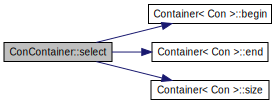
\includegraphics[width=358pt]{class_con_container_a7fb490683bd4733cae3c6428bad9328c_cgraph}
\end{center}
\end{figure}




Here is the caller graph for this function:\nopagebreak
\begin{figure}[H]
\begin{center}
\leavevmode
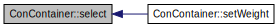
\includegraphics[width=350pt]{class_con_container_a7fb490683bd4733cae3c6428bad9328c_icgraph}
\end{center}
\end{figure}


\hypertarget{class_con_container_aa7f1bbd910afe9c4241e8bd4d5fbc497}{
\index{ConContainer@{ConContainer}!setFrom@{setFrom}}
\index{setFrom@{setFrom}!ConContainer@{ConContainer}}
\subsubsection[{setFrom}]{\setlength{\rightskip}{0pt plus 5cm}bool ConContainer::setFrom (
\begin{DoxyParamCaption}
\item[{{\bf NeuronContainer}}]{neuronContainer}
\end{DoxyParamCaption}
)}}
\label{class_con_container_aa7f1bbd910afe9c4241e8bd4d5fbc497}


Setter of the from fields of the \hyperlink{class_con}{Con} objects related to \hyperlink{class_con_container}{ConContainer}. 

This function provides a convenient way of getting the values of the weight field of those \hyperlink{class_con}{Con} object pointed to by the smart pointer stored in the \hyperlink{class_con_container}{ConContainer} object.


\begin{DoxyParams}{Parameters}
{\em vFrom} & An std::vector$<$NeuronPtr$>$ with the pointers to be set in the from fields of the \hyperlink{class_con_container}{ConContainer} object.\\
\hline
\end{DoxyParams}
\begin{DoxyReturn}{Returns}
true if not exception is thrown
\end{DoxyReturn}

\begin{DoxyCode}
        //================
        //Usage example:
        //================

        // Data set up
                std::vector<int> result;
                ContainerNeuronPtr      neuronContainerPtr( new 
      Container<Neuron>() );
                ConContainerPtr conContainerPtr( new ConContainer() );
                ConPtr  ptC;
                NeuronPtr ptN;

                int ids[]= {10, 20, 30};
                double weights[] = {1.13, 2.22, 3.33 };

                for (int i=0; i<=2 ; i++) {                             // Let's 
      create a vector with three neurons
                        ptN.reset( new Neuron( ids[i] ) );
                        neuronContainerPtr->push_back(ptN);
                }
                for (int i=0; i<=2 ; i++) {                             // and a 
      vector with three connections
                        ptC.reset( new Con() );
                        conContainerPtr->push_back(ptC);
                }
        // Test
                conContainerPtr->setFrom(neuronContainerPtr->load()) ;
                conContainerPtr->show();
                result=conContainerPtr->getId();

        // Now result is a vector that contains the values 10, 20 and 30.
\end{DoxyCode}


\begin{DoxySeeAlso}{See also}
getFrom and the unit test files, e.g. runit.Cpp.ConContainer.R, for further examples. 
\end{DoxySeeAlso}


Definition at line 333 of file ConContainer.cpp.



References Container$<$ T $>$::begin(), Container$<$ T $>$::empty(), Container$<$ Con $>$::size(), and Container$<$ T $>$::size().


\begin{DoxyCode}
{
  BEGIN_RCPP
  if (neuronContainer.empty())
    { throw std::range_error("[ C++ ConContainer::setFrom]: Error, w is empty");}
      
  if (neuronContainer.size() != size())
    {
      throw std::range_error(
          "[C++ ConContainer::setFrom]: Error, neuronContainer.size() != collecti
      on.size()");
    }
  std::vector<NeuronPtr>::iterator itrNeuron = neuronContainer.begin();
  foreach(ConPtr itr , *this)
    {
      itr->setFrom( *itrNeuron );
      itrNeuron++;
    }
  return true;
END_RCPP}
\end{DoxyCode}


Here is the call graph for this function:\nopagebreak
\begin{figure}[H]
\begin{center}
\leavevmode
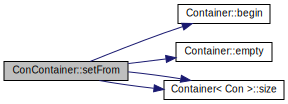
\includegraphics[width=360pt]{class_con_container_aa7f1bbd910afe9c4241e8bd4d5fbc497_cgraph}
\end{center}
\end{figure}


\hypertarget{class_con_container_a2b9d4d12f0e5948b37ccd23445eaef7c}{
\index{ConContainer@{ConContainer}!setWeight@{setWeight}}
\index{setWeight@{setWeight}!ConContainer@{ConContainer}}
\subsubsection[{setWeight}]{\setlength{\rightskip}{0pt plus 5cm}bool ConContainer::setWeight (
\begin{DoxyParamCaption}
\item[{std::vector$<$ double $>$}]{nWeights, }
\item[{std::vector$<$ int $>$}]{nIds}
\end{DoxyParamCaption}
)}}
\label{class_con_container_a2b9d4d12f0e5948b37ccd23445eaef7c}


Setter of the weights of the specified elements from the \hyperlink{class_con_container}{ConContainer} object. 

Provides a convenient way of setting the weights of some \hyperlink{class_con}{Con} objects from the collection field of the \hyperlink{class_con_container}{ConContainer} object.


\begin{DoxyParams}{Parameters}
{\em nWeights} & A numeric (double) vector with the weights to be set in the \hyperlink{class_con}{Con} objects contained in the \hyperlink{class_con_container}{ConContainer} object. \\
\hline
{\em vFrom} & An std::vector$<$int$>$ with the Ids of the connections to select\\
\hline
\end{DoxyParams}
\begin{DoxyReturn}{Returns}
true in case no exception is thrown
\end{DoxyReturn}

\begin{DoxyCode}
        //================
        //Usage example:
        //================

        // Data set up
                std::vector<double> result;
                        std::vector<NeuronPtr> neuronContainer;
                        ConContainerPtr conContainerPtr( new ConContainer() );
                        ConPtr  ptC;
                        NeuronPtr ptN;
                        int ids[]= {11, 10, 9, 3, 4, 5, 6, 7, 8, 2, 1};
                        double weights[]={11.32, 1.26, 2.14, 3.16, 4.14, 5.19, 6.
      18, 7.16, 8.14, 9.12, 10.31};
                        std::vector<double> nWeights;
                        for (int i=0; i<11; i++) {
                        nWeights.push_back(weights[i]);
                        }
                        for (int i=0; i<nWeights.size() ; i++) {                                /
      / Let's create a vector with three neurons
                        ptN.reset( new Neuron( ids[i] ) );
                        neuronContainer.push_back(ptN);
                        }
                        conContainerPtr->buildAndAppend(neuronContainer, nWeights
      );

                        std::vector<int> toSelect;
                        std::vector<double> vNewWeights;
                        toSelect.push_back(1);
                        toSelect.push_back(3);
                        toSelect.push_back(5);
                        toSelect.push_back(7);
                        vNewWeights.push_back(1000.1);
                        vNewWeights.push_back(3000.3);
                        vNewWeights.push_back(5000.5);
                        vNewWeights.push_back(7000.7);
                        conContainerPtr->setWeight(vNewWeights, toSelect);

        // Test
                        result = conContainerPtr->getWeight();
                        return wrap(result);

        // Now, result is a numeric vector with the values  1000.10, 9.12, 3000.3
      0, 4.14, 5000.50, 6.18, 7000.70, 8.14, 2.14, 1.26 and 11.32 .
\end{DoxyCode}


\begin{DoxySeeAlso}{See also}
getWeigth and the unit test files, e.g. runit.Cpp.ConContainer.R, for further examples. 
\end{DoxySeeAlso}


Definition at line 627 of file ConContainer.cpp.



References select().


\begin{DoxyCode}
{
BEGIN_RCPP return select(nIds)->setWeight(nWeights);
END_RCPP
}
\end{DoxyCode}


Here is the call graph for this function:\nopagebreak
\begin{figure}[H]
\begin{center}
\leavevmode
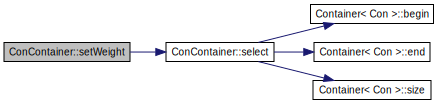
\includegraphics[width=400pt]{class_con_container_a2b9d4d12f0e5948b37ccd23445eaef7c_cgraph}
\end{center}
\end{figure}


\hypertarget{class_con_container_a36dc3c4d86e63eda0a1e9ba17179c0f9}{
\index{ConContainer@{ConContainer}!setWeight@{setWeight}}
\index{setWeight@{setWeight}!ConContainer@{ConContainer}}
\subsubsection[{setWeight}]{\setlength{\rightskip}{0pt plus 5cm}bool ConContainer::setWeight (
\begin{DoxyParamCaption}
\item[{std::vector$<$ double $>$}]{nWeights}
\end{DoxyParamCaption}
)}}
\label{class_con_container_a36dc3c4d86e63eda0a1e9ba17179c0f9}


Setter of the weight field of the \hyperlink{class_con}{Con} objects related to \hyperlink{class_con_container}{ConContainer}. 

This function provides a convenient way of setting the values of the weight field of those \hyperlink{class_con}{Con} objects pointed to by the smart pointer stored in the \hyperlink{class_con_container}{ConContainer} object.


\begin{DoxyParams}{Parameters}
{\em nWeights} & A numeric (double) vector with the weights to be set in the \hyperlink{class_con}{Con} objects contained in the \hyperlink{class_con_container}{ConContainer} object.\\
\hline
\end{DoxyParams}
\begin{DoxyReturn}{Returns}
true in case no exception is thrown
\end{DoxyReturn}

\begin{DoxyCode}
        //================
        //Usage example:
        //================
        // Data set up
                std::vector<double> result;
                        int ids[]= {1, 2, 3};
                        double weights[] = {12.3, 1.2, 2.1 };
                        ConContainer conContainer;
                        std::vector<NeuronPtr> neuronContainer;
                        std::vector<double> nWeights;
                        NeuronPtr ptNeuron;

                        for (int i=0; i<=2; i++) {
                        ptNeuron.reset( new Neuron(ids[1]) );
                        neuronContainer.push_back(ptNeuron);
                        nWeights.push_back(0);                                  /
      / weights are set to 0
                        }
                        conContainer.buildAndAppend(neuronContainer, nWeights);
                        conContainer.show();

                        for (int i=0; i<=2; i++) {
                                nWeights.at(i)=weights[i];
                        }
        // Test
                        conContainer.setWeight(nWeights);                       /
      / weights are set to 12.3, 1.2 and 2.1
                        result=conContainer.getWeight();

        // Now result is a vector that contains the values 12.3, 1.2 and 2.1 .
\end{DoxyCode}


\begin{DoxySeeAlso}{See also}
getWeight and the unit test files, e.g. runit.Cpp.ConContainer.R, for further examples. 
\end{DoxySeeAlso}


Definition at line 270 of file ConContainer.cpp.



References Container$<$ Con $>$::size().


\begin{DoxyCode}
{
  BEGIN_RCPP
  if (nWeights.empty())
    { throw std::range_error("[ C++ ConContainer::setWeight]: Error, nWeights is 
      empty");}
  if (nWeights.size() != size())
    {
      throw std::range_error(
          "[C++ ConContainer::setWeight]: Error, nWeights.size() != collection.si
      ze()");
    }
  std::vector<double>::iterator itrWeight = nWeights.begin();
  foreach (ConPtr itr, *this)
    {
      itr->setWeight( *itrWeight );
      itrWeight++;
    }
  return true;
END_RCPP}
\end{DoxyCode}


Here is the call graph for this function:\nopagebreak
\begin{figure}[H]
\begin{center}
\leavevmode
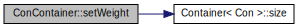
\includegraphics[width=370pt]{class_con_container_a36dc3c4d86e63eda0a1e9ba17179c0f9_cgraph}
\end{center}
\end{figure}


\hypertarget{class_con_container_aac12a3d3604db9ff715503816109470c}{
\index{ConContainer@{ConContainer}!validate@{validate}}
\index{validate@{validate}!ConContainer@{ConContainer}}
\subsubsection[{validate}]{\setlength{\rightskip}{0pt plus 5cm}bool ConContainer::validate (
\begin{DoxyParamCaption}
{}
\end{DoxyParamCaption}
)\hspace{0.3cm}{\ttfamily  \mbox{[}virtual\mbox{]}}}}
\label{class_con_container_aac12a3d3604db9ff715503816109470c}


Object validator. 

This method checks the object for internal coherence. A try / catch mechanism exits normal execution and returns control to the R terminal in case the contents of the \hyperlink{class_con_container}{ConContainer} object are identified as corrupted.

\begin{DoxyReturn}{Returns}
true in case the checks are Ok.
\end{DoxyReturn}

\begin{DoxyExceptions}{Exceptions}
{\em An} & std::range error if weight or from are not finite.\\
\hline
\end{DoxyExceptions}
\begin{DoxySeeAlso}{See also}
The unit test files, e.g., runit.Cpp.ConContainer.R, for usage examples. 
\end{DoxySeeAlso}


Implements \hyperlink{class_container_acfdc5456a2fc854d1830a8a351567928}{Container$<$ Con $>$}.



Definition at line 645 of file ConContainer.cpp.



References getId().


\begin{DoxyCode}
{
  BEGIN_RCPP

  std::vector<int>::iterator itr;
  std::vector<int> vIds = getId();
  sort(vIds.begin(), vIds.end());
  itr = adjacent_find(vIds.begin(), vIds.end());
  if (itr != vIds.end())
    throw std::range_error(
        "[C++ ConContainer::validate]: Error, duplicated Id.");
  Container<Con>::validate();
  return (true);
END_RCPP};
\end{DoxyCode}


Here is the call graph for this function:\nopagebreak
\begin{figure}[H]
\begin{center}
\leavevmode
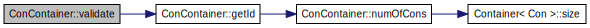
\includegraphics[width=400pt]{class_con_container_aac12a3d3604db9ff715503816109470c_cgraph}
\end{center}
\end{figure}




The documentation for this class was generated from the following files:\begin{DoxyCompactItemize}
\item 
pkg/AMORE/src/old/\hyperlink{_con_container_8h}{ConContainer.h}\item 
pkg/AMORE/src/old/\hyperlink{_con_container_8cpp}{ConContainer.cpp}\end{DoxyCompactItemize}

\hypertarget{class_container}{
\section{Container$<$ T $>$ Class Template Reference}
\label{class_container}\index{Container@{Container}}
}


class \hyperlink{class_container}{Container} -\/  




{\ttfamily \#include $<$Container.h$>$}



Inheritance diagram for Container$<$ T $>$:
\nopagebreak
\begin{figure}[H]
\begin{center}
\leavevmode
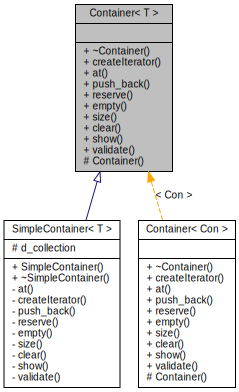
\includegraphics[width=196pt]{class_container__inherit__graph}
\end{center}
\end{figure}
\subsection*{Public Member Functions}
\begin{DoxyCompactItemize}
\item 
virtual \hyperlink{class_container_ac190e8e99e5a92ef02390027765cbbb6}{$\sim$Container} ()
\item 
virtual boost::shared\_\-ptr$<$ \hyperlink{class_iterator}{Iterator}$<$ T $>$ $>$ \hyperlink{class_container_a18a0a70153781d3d94526bc09fcbedb8}{createIterator} ()=0
\item 
virtual T \hyperlink{class_container_a8aed06783f7cd0749f796c64e64626e7}{at} (size\_\-type element)=0
\item 
virtual void \hyperlink{class_container_a12ffe2d2dbbcd78b6b293756004bd6e0}{push\_\-back} (T const \&const\_\-reference)=0
\item 
virtual void \hyperlink{class_container_a5f70fb0d821a8db9a0733aafe9ef35ac}{reserve} (int n)=0
\item 
virtual bool \hyperlink{class_container_a123dcd25b363ab92ac8bfa8b4c4061a4}{empty} ()=0
\item 
virtual size\_\-type \hyperlink{class_container_a1eebc7b5cbb0c574cb1aef87c2ddba36}{size} ()=0
\item 
virtual void \hyperlink{class_container_ac27f3554d6ac6ecb227ead060ff1f8a2}{clear} ()=0
\item 
virtual void \hyperlink{class_container_a5ee85af656e60863a7e4c1f7f9c484f4}{show} ()=0
\item 
virtual bool \hyperlink{class_container_abbd8ca2714a550351442f4410cf5736d}{validate} ()=0
\end{DoxyCompactItemize}
\subsection*{Protected Member Functions}
\begin{DoxyCompactItemize}
\item 
\hyperlink{class_container_ab17ce1f67243b28abcd4c8113a72524c}{Container} ()
\end{DoxyCompactItemize}


\subsection{Detailed Description}
\subsubsection*{template$<$typename T$>$class Container$<$ T $>$}

class \hyperlink{class_container}{Container} -\/ 

Definition at line 5 of file Container.h.



\subsection{Constructor \& Destructor Documentation}
\hypertarget{class_container_ac190e8e99e5a92ef02390027765cbbb6}{
\index{Container@{Container}!$\sim$Container@{$\sim$Container}}
\index{$\sim$Container@{$\sim$Container}!Container@{Container}}
\subsubsection[{$\sim$Container}]{\setlength{\rightskip}{0pt plus 5cm}template$<$typename T $>$ virtual {\bf Container}$<$ T $>$::$\sim${\bf Container} (
\begin{DoxyParamCaption}
{}
\end{DoxyParamCaption}
)\hspace{0.3cm}{\ttfamily  \mbox{[}virtual\mbox{]}}}}
\label{class_container_ac190e8e99e5a92ef02390027765cbbb6}
\hypertarget{class_container_ab17ce1f67243b28abcd4c8113a72524c}{
\index{Container@{Container}!Container@{Container}}
\index{Container@{Container}!Container@{Container}}
\subsubsection[{Container}]{\setlength{\rightskip}{0pt plus 5cm}template$<$typename T $>$ {\bf Container}$<$ T $>$::{\bf Container} (
\begin{DoxyParamCaption}
{}
\end{DoxyParamCaption}
)\hspace{0.3cm}{\ttfamily  \mbox{[}protected\mbox{]}}}}
\label{class_container_ab17ce1f67243b28abcd4c8113a72524c}


\subsection{Member Function Documentation}
\hypertarget{class_container_a8aed06783f7cd0749f796c64e64626e7}{
\index{Container@{Container}!at@{at}}
\index{at@{at}!Container@{Container}}
\subsubsection[{at}]{\setlength{\rightskip}{0pt plus 5cm}template$<$typename T $>$ virtual T {\bf Container}$<$ T $>$::at (
\begin{DoxyParamCaption}
\item[{size\_\-type}]{element}
\end{DoxyParamCaption}
)\hspace{0.3cm}{\ttfamily  \mbox{[}pure virtual\mbox{]}}}}
\label{class_container_a8aed06783f7cd0749f796c64e64626e7}


Implemented in \hyperlink{class_simple_container_a2e8f56f3af1e0ffb1fcd54d05d82c477}{SimpleContainer$<$ T $>$}.

\hypertarget{class_container_ac27f3554d6ac6ecb227ead060ff1f8a2}{
\index{Container@{Container}!clear@{clear}}
\index{clear@{clear}!Container@{Container}}
\subsubsection[{clear}]{\setlength{\rightskip}{0pt plus 5cm}template$<$typename T $>$ virtual void {\bf Container}$<$ T $>$::clear (
\begin{DoxyParamCaption}
{}
\end{DoxyParamCaption}
)\hspace{0.3cm}{\ttfamily  \mbox{[}pure virtual\mbox{]}}}}
\label{class_container_ac27f3554d6ac6ecb227ead060ff1f8a2}


Implemented in \hyperlink{class_simple_container_ae3ee6cb18f1dd33ab5de4f9854ce245f}{SimpleContainer$<$ T $>$}.

\hypertarget{class_container_a18a0a70153781d3d94526bc09fcbedb8}{
\index{Container@{Container}!createIterator@{createIterator}}
\index{createIterator@{createIterator}!Container@{Container}}
\subsubsection[{createIterator}]{\setlength{\rightskip}{0pt plus 5cm}template$<$typename T $>$ virtual boost::shared\_\-ptr$<$ {\bf Iterator}$<$T$>$ $>$ {\bf Container}$<$ T $>$::createIterator (
\begin{DoxyParamCaption}
{}
\end{DoxyParamCaption}
)\hspace{0.3cm}{\ttfamily  \mbox{[}pure virtual\mbox{]}}}}
\label{class_container_a18a0a70153781d3d94526bc09fcbedb8}


Implemented in \hyperlink{class_simple_container_a4e46f5cb32231deaf9aa9bb7f871d09e}{SimpleContainer$<$ T $>$}.

\hypertarget{class_container_a123dcd25b363ab92ac8bfa8b4c4061a4}{
\index{Container@{Container}!empty@{empty}}
\index{empty@{empty}!Container@{Container}}
\subsubsection[{empty}]{\setlength{\rightskip}{0pt plus 5cm}template$<$typename T $>$ virtual bool {\bf Container}$<$ T $>$::empty (
\begin{DoxyParamCaption}
{}
\end{DoxyParamCaption}
)\hspace{0.3cm}{\ttfamily  \mbox{[}pure virtual\mbox{]}}}}
\label{class_container_a123dcd25b363ab92ac8bfa8b4c4061a4}


Implemented in \hyperlink{class_simple_container_ac2966f33796f69c290a84361a578ed08}{SimpleContainer$<$ T $>$}.

\hypertarget{class_container_a12ffe2d2dbbcd78b6b293756004bd6e0}{
\index{Container@{Container}!push\_\-back@{push\_\-back}}
\index{push\_\-back@{push\_\-back}!Container@{Container}}
\subsubsection[{push\_\-back}]{\setlength{\rightskip}{0pt plus 5cm}template$<$typename T $>$ virtual void {\bf Container}$<$ T $>$::push\_\-back (
\begin{DoxyParamCaption}
\item[{T const \&}]{const\_\-reference}
\end{DoxyParamCaption}
)\hspace{0.3cm}{\ttfamily  \mbox{[}pure virtual\mbox{]}}}}
\label{class_container_a12ffe2d2dbbcd78b6b293756004bd6e0}


Implemented in \hyperlink{class_simple_container_a53466966297b3f0a707e025b3721004a}{SimpleContainer$<$ T $>$}.

\hypertarget{class_container_a5f70fb0d821a8db9a0733aafe9ef35ac}{
\index{Container@{Container}!reserve@{reserve}}
\index{reserve@{reserve}!Container@{Container}}
\subsubsection[{reserve}]{\setlength{\rightskip}{0pt plus 5cm}template$<$typename T $>$ virtual void {\bf Container}$<$ T $>$::reserve (
\begin{DoxyParamCaption}
\item[{int}]{n}
\end{DoxyParamCaption}
)\hspace{0.3cm}{\ttfamily  \mbox{[}pure virtual\mbox{]}}}}
\label{class_container_a5f70fb0d821a8db9a0733aafe9ef35ac}


Implemented in \hyperlink{class_simple_container_a4bca44e6a9cef9d57627218c0a180d8a}{SimpleContainer$<$ T $>$}.

\hypertarget{class_container_a5ee85af656e60863a7e4c1f7f9c484f4}{
\index{Container@{Container}!show@{show}}
\index{show@{show}!Container@{Container}}
\subsubsection[{show}]{\setlength{\rightskip}{0pt plus 5cm}template$<$typename T $>$ virtual void {\bf Container}$<$ T $>$::show (
\begin{DoxyParamCaption}
{}
\end{DoxyParamCaption}
)\hspace{0.3cm}{\ttfamily  \mbox{[}pure virtual\mbox{]}}}}
\label{class_container_a5ee85af656e60863a7e4c1f7f9c484f4}


Implemented in \hyperlink{class_simple_container_af4d591e2c3a44ae016e01e3d07d1e9ac}{SimpleContainer$<$ T $>$}.

\hypertarget{class_container_a1eebc7b5cbb0c574cb1aef87c2ddba36}{
\index{Container@{Container}!size@{size}}
\index{size@{size}!Container@{Container}}
\subsubsection[{size}]{\setlength{\rightskip}{0pt plus 5cm}template$<$typename T $>$ virtual size\_\-type {\bf Container}$<$ T $>$::size (
\begin{DoxyParamCaption}
{}
\end{DoxyParamCaption}
)\hspace{0.3cm}{\ttfamily  \mbox{[}pure virtual\mbox{]}}}}
\label{class_container_a1eebc7b5cbb0c574cb1aef87c2ddba36}


Implemented in \hyperlink{class_simple_container_a2fdb3580e1728e6e2ba6ef77c0bce63e}{SimpleContainer$<$ T $>$}.

\hypertarget{class_container_abbd8ca2714a550351442f4410cf5736d}{
\index{Container@{Container}!validate@{validate}}
\index{validate@{validate}!Container@{Container}}
\subsubsection[{validate}]{\setlength{\rightskip}{0pt plus 5cm}template$<$typename T $>$ virtual bool {\bf Container}$<$ T $>$::validate (
\begin{DoxyParamCaption}
{}
\end{DoxyParamCaption}
)\hspace{0.3cm}{\ttfamily  \mbox{[}pure virtual\mbox{]}}}}
\label{class_container_abbd8ca2714a550351442f4410cf5736d}


Implemented in \hyperlink{class_simple_container_ac7cae8eaac2dc0a69138b65f679bd16a}{SimpleContainer$<$ T $>$}.



The documentation for this class was generated from the following file:\begin{DoxyCompactItemize}
\item 
/Users/mcasl/pc-\/ule/Trabajo/investigacion/AMORE/AMORE-\/WC/AMORE-\/WC/pkg/AMORE/src/classHeaders/\hyperlink{_container_8h}{Container.h}\end{DoxyCompactItemize}

\hypertarget{class_container_interface}{
\section{ContainerInterface$<$ T $>$ Class Template Reference}
\label{class_container_interface}\index{ContainerInterface@{ContainerInterface}}
}


class \hyperlink{class_container_interface}{ContainerInterface} -\/  




{\ttfamily \#include $<$ContainerInterface.h$>$}



Inheritance diagram for ContainerInterface$<$ T $>$:
\nopagebreak
\begin{figure}[H]
\begin{center}
\leavevmode
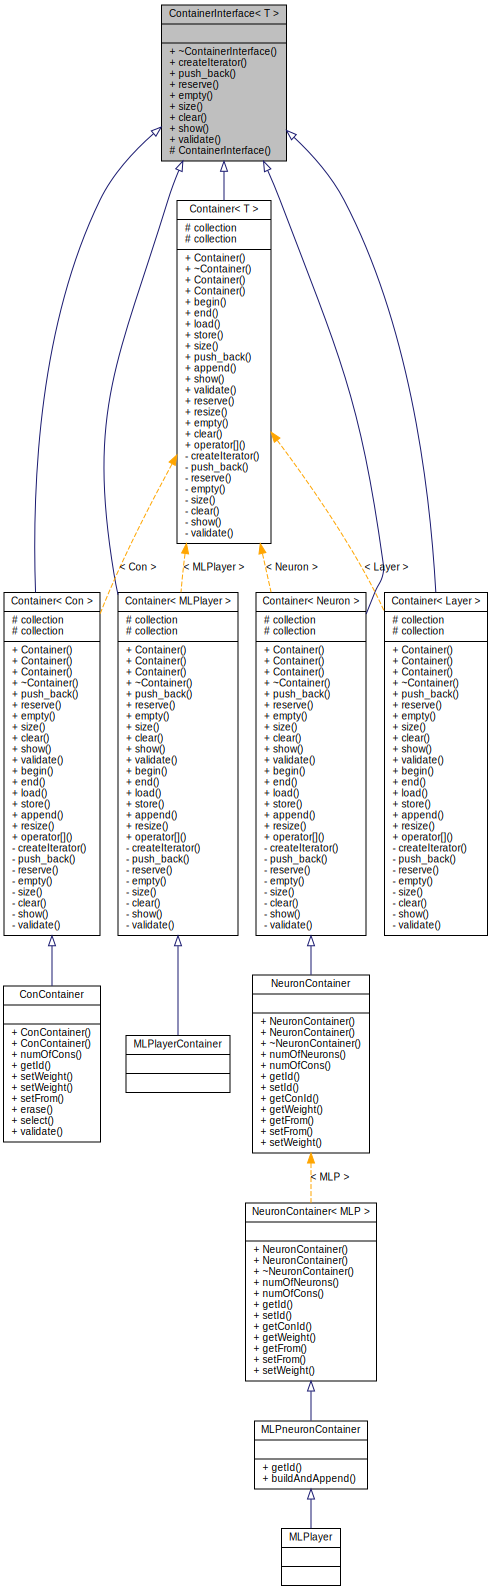
\includegraphics[height=600pt]{class_container_interface__inherit__graph}
\end{center}
\end{figure}
\subsection*{Public Member Functions}
\begin{DoxyCompactItemize}
\item 
virtual \hyperlink{class_container_interface_a5e7db3193461a44c1e05c1ecc9caed95}{$\sim$ContainerInterface} ()
\item 
virtual boost::shared\_\-ptr$<$ \hyperlink{class_iterator_interface}{IteratorInterface}$<$ T $>$ $>$ \hyperlink{class_container_interface_a70769b558499b31462fa291db3d13b30}{createIterator} ()=0
\item 
virtual void \hyperlink{class_container_interface_a261e2fb8c71777d127052d2aef60b182}{push\_\-back} (T const \&const\_\-reference)=0
\item 
virtual void \hyperlink{class_container_interface_aa2023fa458c061c5293be5364bc1d440}{reserve} (int n)=0
\item 
virtual bool \hyperlink{class_container_interface_a47b337e49cd7b9f75d6964238fa7e8bc}{empty} ()=0
\item 
virtual size\_\-type \hyperlink{class_container_interface_aa194c58e394eeb6ae6655f14ab74823a}{size} ()=0
\item 
virtual void \hyperlink{class_container_interface_a321e214f22940891f51f4fd45ed8d106}{clear} ()=0
\item 
virtual void \hyperlink{class_container_interface_a09d9a76fd7e867951bdced07134259a3}{show} ()=0
\item 
virtual bool \hyperlink{class_container_interface_a550edb62b31da71cd66270d87bc81c97}{validate} ()=0
\end{DoxyCompactItemize}
\subsection*{Protected Member Functions}
\begin{DoxyCompactItemize}
\item 
\hyperlink{class_container_interface_a1203fe4cd19f556845500ad07a0a16d5}{ContainerInterface} ()
\end{DoxyCompactItemize}


\subsection{Detailed Description}
\subsubsection*{template$<$typename T$>$class ContainerInterface$<$ T $>$}

class \hyperlink{class_container_interface}{ContainerInterface} -\/ 

Definition at line 5 of file ContainerInterface.h.



\subsection{Constructor \& Destructor Documentation}
\hypertarget{class_container_interface_a5e7db3193461a44c1e05c1ecc9caed95}{
\index{ContainerInterface@{ContainerInterface}!$\sim$ContainerInterface@{$\sim$ContainerInterface}}
\index{$\sim$ContainerInterface@{$\sim$ContainerInterface}!ContainerInterface@{ContainerInterface}}
\subsubsection[{$\sim$ContainerInterface}]{\setlength{\rightskip}{0pt plus 5cm}template$<$typename T $>$ {\bf ContainerInterface}$<$ T $>$::$\sim${\bf ContainerInterface} (
\begin{DoxyParamCaption}
{}
\end{DoxyParamCaption}
)\hspace{0.3cm}{\ttfamily  \mbox{[}virtual\mbox{]}}}}
\label{class_container_interface_a5e7db3193461a44c1e05c1ecc9caed95}


Definition at line 10 of file containerInterface.cpp.


\begin{DoxyCode}
  {
  }
\end{DoxyCode}
\hypertarget{class_container_interface_a1203fe4cd19f556845500ad07a0a16d5}{
\index{ContainerInterface@{ContainerInterface}!ContainerInterface@{ContainerInterface}}
\index{ContainerInterface@{ContainerInterface}!ContainerInterface@{ContainerInterface}}
\subsubsection[{ContainerInterface}]{\setlength{\rightskip}{0pt plus 5cm}template$<$typename T $>$ {\bf ContainerInterface}$<$ T $>$::{\bf ContainerInterface} (
\begin{DoxyParamCaption}
{}
\end{DoxyParamCaption}
)\hspace{0.3cm}{\ttfamily  \mbox{[}protected\mbox{]}}}}
\label{class_container_interface_a1203fe4cd19f556845500ad07a0a16d5}


Definition at line 4 of file containerInterface.cpp.


\begin{DoxyCode}
  {
  }
\end{DoxyCode}


\subsection{Member Function Documentation}
\hypertarget{class_container_interface_a321e214f22940891f51f4fd45ed8d106}{
\index{ContainerInterface@{ContainerInterface}!clear@{clear}}
\index{clear@{clear}!ContainerInterface@{ContainerInterface}}
\subsubsection[{clear}]{\setlength{\rightskip}{0pt plus 5cm}template$<$typename T $>$ virtual void {\bf ContainerInterface}$<$ T $>$::clear (
\begin{DoxyParamCaption}
{}
\end{DoxyParamCaption}
)\hspace{0.3cm}{\ttfamily  \mbox{[}pure virtual\mbox{]}}}}
\label{class_container_interface_a321e214f22940891f51f4fd45ed8d106}


Implemented in \hyperlink{class_container_aab0690d44c8e04614cea46935ff49e7a}{Container$<$ T $>$}, \hyperlink{class_container_aab0690d44c8e04614cea46935ff49e7a}{Container$<$ T $>$}, \hyperlink{class_container_aab0690d44c8e04614cea46935ff49e7a}{Container$<$ MLPlayer $>$}, \hyperlink{class_container_aab0690d44c8e04614cea46935ff49e7a}{Container$<$ MLPlayer $>$}, \hyperlink{class_container_aab0690d44c8e04614cea46935ff49e7a}{Container$<$ Con $>$}, \hyperlink{class_container_aab0690d44c8e04614cea46935ff49e7a}{Container$<$ Con $>$}, \hyperlink{class_container_aab0690d44c8e04614cea46935ff49e7a}{Container$<$ Layer $>$}, \hyperlink{class_container_aab0690d44c8e04614cea46935ff49e7a}{Container$<$ Layer $>$}, \hyperlink{class_container_aab0690d44c8e04614cea46935ff49e7a}{Container$<$ Neuron $>$}, and \hyperlink{class_container_aab0690d44c8e04614cea46935ff49e7a}{Container$<$ Neuron $>$}.

\hypertarget{class_container_interface_a70769b558499b31462fa291db3d13b30}{
\index{ContainerInterface@{ContainerInterface}!createIterator@{createIterator}}
\index{createIterator@{createIterator}!ContainerInterface@{ContainerInterface}}
\subsubsection[{createIterator}]{\setlength{\rightskip}{0pt plus 5cm}template$<$typename T $>$ virtual boost::shared\_\-ptr$<$ {\bf IteratorInterface}$<$T$>$ $>$ {\bf ContainerInterface}$<$ T $>$::createIterator (
\begin{DoxyParamCaption}
{}
\end{DoxyParamCaption}
)\hspace{0.3cm}{\ttfamily  \mbox{[}pure virtual\mbox{]}}}}
\label{class_container_interface_a70769b558499b31462fa291db3d13b30}


Implemented in \hyperlink{class_container_ad3525eb1902b1e71cf20db4423d8bb9a}{Container$<$ T $>$}, \hyperlink{class_container_ad3525eb1902b1e71cf20db4423d8bb9a}{Container$<$ MLPlayer $>$}, \hyperlink{class_container_ad3525eb1902b1e71cf20db4423d8bb9a}{Container$<$ Con $>$}, \hyperlink{class_container_ad3525eb1902b1e71cf20db4423d8bb9a}{Container$<$ Layer $>$}, and \hyperlink{class_container_ad3525eb1902b1e71cf20db4423d8bb9a}{Container$<$ Neuron $>$}.

\hypertarget{class_container_interface_a47b337e49cd7b9f75d6964238fa7e8bc}{
\index{ContainerInterface@{ContainerInterface}!empty@{empty}}
\index{empty@{empty}!ContainerInterface@{ContainerInterface}}
\subsubsection[{empty}]{\setlength{\rightskip}{0pt plus 5cm}template$<$typename T $>$ virtual bool {\bf ContainerInterface}$<$ T $>$::empty (
\begin{DoxyParamCaption}
{}
\end{DoxyParamCaption}
)\hspace{0.3cm}{\ttfamily  \mbox{[}pure virtual\mbox{]}}}}
\label{class_container_interface_a47b337e49cd7b9f75d6964238fa7e8bc}


Implemented in \hyperlink{class_container_ab8e09c25f519687468ef5b9f0fae9b3e}{Container$<$ T $>$}, \hyperlink{class_container_ab8e09c25f519687468ef5b9f0fae9b3e}{Container$<$ T $>$}, \hyperlink{class_container_ab8e09c25f519687468ef5b9f0fae9b3e}{Container$<$ MLPlayer $>$}, \hyperlink{class_container_ab8e09c25f519687468ef5b9f0fae9b3e}{Container$<$ MLPlayer $>$}, \hyperlink{class_container_ab8e09c25f519687468ef5b9f0fae9b3e}{Container$<$ Con $>$}, \hyperlink{class_container_ab8e09c25f519687468ef5b9f0fae9b3e}{Container$<$ Con $>$}, \hyperlink{class_container_ab8e09c25f519687468ef5b9f0fae9b3e}{Container$<$ Layer $>$}, \hyperlink{class_container_ab8e09c25f519687468ef5b9f0fae9b3e}{Container$<$ Layer $>$}, \hyperlink{class_container_ab8e09c25f519687468ef5b9f0fae9b3e}{Container$<$ Neuron $>$}, and \hyperlink{class_container_ab8e09c25f519687468ef5b9f0fae9b3e}{Container$<$ Neuron $>$}.

\hypertarget{class_container_interface_a261e2fb8c71777d127052d2aef60b182}{
\index{ContainerInterface@{ContainerInterface}!push\_\-back@{push\_\-back}}
\index{push\_\-back@{push\_\-back}!ContainerInterface@{ContainerInterface}}
\subsubsection[{push\_\-back}]{\setlength{\rightskip}{0pt plus 5cm}template$<$typename T $>$ virtual void {\bf ContainerInterface}$<$ T $>$::push\_\-back (
\begin{DoxyParamCaption}
\item[{T const \&}]{const\_\-reference}
\end{DoxyParamCaption}
)\hspace{0.3cm}{\ttfamily  \mbox{[}pure virtual\mbox{]}}}}
\label{class_container_interface_a261e2fb8c71777d127052d2aef60b182}


Implemented in \hyperlink{class_container_ace7da25fd798b831d475b37fb58a9d78}{Container$<$ T $>$}.

\hypertarget{class_container_interface_aa2023fa458c061c5293be5364bc1d440}{
\index{ContainerInterface@{ContainerInterface}!reserve@{reserve}}
\index{reserve@{reserve}!ContainerInterface@{ContainerInterface}}
\subsubsection[{reserve}]{\setlength{\rightskip}{0pt plus 5cm}template$<$typename T $>$ virtual void {\bf ContainerInterface}$<$ T $>$::reserve (
\begin{DoxyParamCaption}
\item[{int}]{n}
\end{DoxyParamCaption}
)\hspace{0.3cm}{\ttfamily  \mbox{[}pure virtual\mbox{]}}}}
\label{class_container_interface_aa2023fa458c061c5293be5364bc1d440}


Implemented in \hyperlink{class_container_aa3cbae68ebeed649c52eb3805a30fb75}{Container$<$ T $>$}, \hyperlink{class_container_aa3cbae68ebeed649c52eb3805a30fb75}{Container$<$ T $>$}, \hyperlink{class_container_aa3cbae68ebeed649c52eb3805a30fb75}{Container$<$ MLPlayer $>$}, \hyperlink{class_container_aa3cbae68ebeed649c52eb3805a30fb75}{Container$<$ MLPlayer $>$}, \hyperlink{class_container_aa3cbae68ebeed649c52eb3805a30fb75}{Container$<$ Con $>$}, \hyperlink{class_container_aa3cbae68ebeed649c52eb3805a30fb75}{Container$<$ Con $>$}, \hyperlink{class_container_aa3cbae68ebeed649c52eb3805a30fb75}{Container$<$ Layer $>$}, \hyperlink{class_container_aa3cbae68ebeed649c52eb3805a30fb75}{Container$<$ Layer $>$}, \hyperlink{class_container_aa3cbae68ebeed649c52eb3805a30fb75}{Container$<$ Neuron $>$}, and \hyperlink{class_container_aa3cbae68ebeed649c52eb3805a30fb75}{Container$<$ Neuron $>$}.

\hypertarget{class_container_interface_a09d9a76fd7e867951bdced07134259a3}{
\index{ContainerInterface@{ContainerInterface}!show@{show}}
\index{show@{show}!ContainerInterface@{ContainerInterface}}
\subsubsection[{show}]{\setlength{\rightskip}{0pt plus 5cm}template$<$typename T $>$ virtual void {\bf ContainerInterface}$<$ T $>$::show (
\begin{DoxyParamCaption}
{}
\end{DoxyParamCaption}
)\hspace{0.3cm}{\ttfamily  \mbox{[}pure virtual\mbox{]}}}}
\label{class_container_interface_a09d9a76fd7e867951bdced07134259a3}


Implemented in \hyperlink{class_container_ad72379ee222b073a5eecec7fc1bedfc2}{Container$<$ T $>$}, \hyperlink{class_container_ad72379ee222b073a5eecec7fc1bedfc2}{Container$<$ T $>$}, \hyperlink{class_container_ad72379ee222b073a5eecec7fc1bedfc2}{Container$<$ MLPlayer $>$}, \hyperlink{class_container_ad72379ee222b073a5eecec7fc1bedfc2}{Container$<$ MLPlayer $>$}, \hyperlink{class_container_ad72379ee222b073a5eecec7fc1bedfc2}{Container$<$ Con $>$}, \hyperlink{class_container_ad72379ee222b073a5eecec7fc1bedfc2}{Container$<$ Con $>$}, \hyperlink{class_container_ad72379ee222b073a5eecec7fc1bedfc2}{Container$<$ Layer $>$}, \hyperlink{class_container_ad72379ee222b073a5eecec7fc1bedfc2}{Container$<$ Layer $>$}, \hyperlink{class_container_ad72379ee222b073a5eecec7fc1bedfc2}{Container$<$ Neuron $>$}, and \hyperlink{class_container_ad72379ee222b073a5eecec7fc1bedfc2}{Container$<$ Neuron $>$}.

\hypertarget{class_container_interface_aa194c58e394eeb6ae6655f14ab74823a}{
\index{ContainerInterface@{ContainerInterface}!size@{size}}
\index{size@{size}!ContainerInterface@{ContainerInterface}}
\subsubsection[{size}]{\setlength{\rightskip}{0pt plus 5cm}template$<$typename T $>$ virtual size\_\-type {\bf ContainerInterface}$<$ T $>$::size (
\begin{DoxyParamCaption}
{}
\end{DoxyParamCaption}
)\hspace{0.3cm}{\ttfamily  \mbox{[}pure virtual\mbox{]}}}}
\label{class_container_interface_aa194c58e394eeb6ae6655f14ab74823a}


Implemented in \hyperlink{class_container_a842c3d9eca81b78b59112fde9707b091}{Container$<$ T $>$}, \hyperlink{class_container_a842c3d9eca81b78b59112fde9707b091}{Container$<$ T $>$}, \hyperlink{class_container_a842c3d9eca81b78b59112fde9707b091}{Container$<$ MLPlayer $>$}, \hyperlink{class_container_a842c3d9eca81b78b59112fde9707b091}{Container$<$ MLPlayer $>$}, \hyperlink{class_container_a842c3d9eca81b78b59112fde9707b091}{Container$<$ Con $>$}, \hyperlink{class_container_a842c3d9eca81b78b59112fde9707b091}{Container$<$ Con $>$}, \hyperlink{class_container_a842c3d9eca81b78b59112fde9707b091}{Container$<$ Layer $>$}, \hyperlink{class_container_a842c3d9eca81b78b59112fde9707b091}{Container$<$ Layer $>$}, \hyperlink{class_container_a842c3d9eca81b78b59112fde9707b091}{Container$<$ Neuron $>$}, and \hyperlink{class_container_a842c3d9eca81b78b59112fde9707b091}{Container$<$ Neuron $>$}.

\hypertarget{class_container_interface_a550edb62b31da71cd66270d87bc81c97}{
\index{ContainerInterface@{ContainerInterface}!validate@{validate}}
\index{validate@{validate}!ContainerInterface@{ContainerInterface}}
\subsubsection[{validate}]{\setlength{\rightskip}{0pt plus 5cm}template$<$typename T $>$ virtual bool {\bf ContainerInterface}$<$ T $>$::validate (
\begin{DoxyParamCaption}
{}
\end{DoxyParamCaption}
)\hspace{0.3cm}{\ttfamily  \mbox{[}pure virtual\mbox{]}}}}
\label{class_container_interface_a550edb62b31da71cd66270d87bc81c97}


Implemented in \hyperlink{class_container_aa99a036fd0fe6d6b82ba558157e557d3}{Container$<$ T $>$}, \hyperlink{class_con_container_aac12a3d3604db9ff715503816109470c}{ConContainer}, \hyperlink{class_container_aa99a036fd0fe6d6b82ba558157e557d3}{Container$<$ T $>$}, \hyperlink{class_container_aa99a036fd0fe6d6b82ba558157e557d3}{Container$<$ MLPlayer $>$}, \hyperlink{class_container_aa99a036fd0fe6d6b82ba558157e557d3}{Container$<$ MLPlayer $>$}, \hyperlink{class_container_aa99a036fd0fe6d6b82ba558157e557d3}{Container$<$ Con $>$}, \hyperlink{class_container_aa99a036fd0fe6d6b82ba558157e557d3}{Container$<$ Con $>$}, \hyperlink{class_container_aa99a036fd0fe6d6b82ba558157e557d3}{Container$<$ Layer $>$}, \hyperlink{class_container_aa99a036fd0fe6d6b82ba558157e557d3}{Container$<$ Layer $>$}, \hyperlink{class_container_aa99a036fd0fe6d6b82ba558157e557d3}{Container$<$ Neuron $>$}, and \hyperlink{class_container_aa99a036fd0fe6d6b82ba558157e557d3}{Container$<$ Neuron $>$}.



The documentation for this class was generated from the following files:\begin{DoxyCompactItemize}
\item 
pkg/AMORE/src/dia/\hyperlink{_container_interface_8h}{ContainerInterface.h}\item 
pkg/AMORE/src/\hyperlink{container_interface_8cpp}{containerInterface.cpp}\end{DoxyCompactItemize}

\hypertarget{class_container_iterator}{
\section{ContainerIterator$<$ T $>$ Class Template Reference}
\label{class_container_iterator}\index{ContainerIterator@{ContainerIterator}}
}


class \hyperlink{class_container_iterator}{ContainerIterator} -\/  




{\ttfamily \#include $<$ContainerIterator.h$>$}



Inheritance diagram for ContainerIterator$<$ T $>$:
\nopagebreak
\begin{figure}[H]
\begin{center}
\leavevmode
\includegraphics[width=198pt]{class_container_iterator__inherit__graph}
\end{center}
\end{figure}


Collaboration diagram for ContainerIterator$<$ T $>$:
\nopagebreak
\begin{figure}[H]
\begin{center}
\leavevmode
\includegraphics[width=198pt]{class_container_iterator__coll__graph}
\end{center}
\end{figure}
\subsection*{Public Member Functions}
\begin{DoxyCompactItemize}
\item 
\hyperlink{class_container_iterator_a5cc7e5a75c276e224706891547e3cf24}{ContainerIterator} ()
\item 
\hyperlink{class_container_iterator_a448896907e42b5676b9cccd0b59e0e43}{$\sim$ContainerIterator} ()
\item 
void \hyperlink{class_container_iterator_a98924935aa2d0b5f1d3bdbb8b3bc0a69}{first} ()
\item 
void \hyperlink{class_container_iterator_ae9996be7cbe4ada65c214372da509049}{next} ()
\item 
bool \hyperlink{class_container_iterator_a533dcd7d4c59663c0ae99f67f4b5e9c6}{isDone} ()
\item 
T \hyperlink{class_container_iterator_a088e991e5eade5740290342a49d71467}{currentItem} ()
\end{DoxyCompactItemize}
\subsection*{Private Attributes}
\begin{DoxyCompactItemize}
\item 
\hyperlink{class_container}{Container}$<$ T $>$ $\ast$ \hyperlink{class_container_iterator_a572dccca78e6c158c4366c13a4447be5}{d\_\-container}
\item 
std::vector$<$ T $>$::iterator \hyperlink{class_container_iterator_a129eade25e86d86d07e1bbb29dd961d6}{d\_\-iterator}
\end{DoxyCompactItemize}
\subsection*{Friends}
\begin{DoxyCompactItemize}
\item 
class \hyperlink{class_container_iterator_a65d024049df91b92de00b0d6830aa657}{Container$<$ T $>$}
\end{DoxyCompactItemize}


\subsection{Detailed Description}
\subsubsection*{template$<$typename T$>$class ContainerIterator$<$ T $>$}

class \hyperlink{class_container_iterator}{ContainerIterator} -\/ 

Definition at line 6 of file ContainerIterator.h.



\subsection{Constructor \& Destructor Documentation}
\hypertarget{class_container_iterator_a5cc7e5a75c276e224706891547e3cf24}{
\index{ContainerIterator@{ContainerIterator}!ContainerIterator@{ContainerIterator}}
\index{ContainerIterator@{ContainerIterator}!ContainerIterator@{ContainerIterator}}
\subsubsection[{ContainerIterator}]{\setlength{\rightskip}{0pt plus 5cm}template$<$typename T $>$ {\bf ContainerIterator}$<$ T $>$::{\bf ContainerIterator} (
\begin{DoxyParamCaption}
{}
\end{DoxyParamCaption}
)}}
\label{class_container_iterator_a5cc7e5a75c276e224706891547e3cf24}


Definition at line 4 of file ContainerIterator.cpp.


\begin{DoxyCode}
  {
  }
\end{DoxyCode}
\hypertarget{class_container_iterator_a448896907e42b5676b9cccd0b59e0e43}{
\index{ContainerIterator@{ContainerIterator}!$\sim$ContainerIterator@{$\sim$ContainerIterator}}
\index{$\sim$ContainerIterator@{$\sim$ContainerIterator}!ContainerIterator@{ContainerIterator}}
\subsubsection[{$\sim$ContainerIterator}]{\setlength{\rightskip}{0pt plus 5cm}template$<$typename T $>$ {\bf ContainerIterator}$<$ T $>$::$\sim${\bf ContainerIterator} (
\begin{DoxyParamCaption}
{}
\end{DoxyParamCaption}
)}}
\label{class_container_iterator_a448896907e42b5676b9cccd0b59e0e43}


Definition at line 9 of file ContainerIterator.cpp.


\begin{DoxyCode}
  {
  }
\end{DoxyCode}


\subsection{Member Function Documentation}
\hypertarget{class_container_iterator_a088e991e5eade5740290342a49d71467}{
\index{ContainerIterator@{ContainerIterator}!currentItem@{currentItem}}
\index{currentItem@{currentItem}!ContainerIterator@{ContainerIterator}}
\subsubsection[{currentItem}]{\setlength{\rightskip}{0pt plus 5cm}template$<$typename T $>$ T {\bf ContainerIterator}$<$ T $>$::currentItem (
\begin{DoxyParamCaption}
{}
\end{DoxyParamCaption}
)\hspace{0.3cm}{\ttfamily  \mbox{[}virtual\mbox{]}}}}
\label{class_container_iterator_a088e991e5eade5740290342a49d71467}


Implements \hyperlink{class_iterator_interface_a1724076d202e22aefd13325c06a91033}{IteratorInterface$<$ T $>$}.



Definition at line 37 of file ContainerIterator.cpp.



References ContainerIterator$<$ T $>$::d\_\-iterator.


\begin{DoxyCode}
  {
    return *d_iterator;
  }
\end{DoxyCode}
\hypertarget{class_container_iterator_a98924935aa2d0b5f1d3bdbb8b3bc0a69}{
\index{ContainerIterator@{ContainerIterator}!first@{first}}
\index{first@{first}!ContainerIterator@{ContainerIterator}}
\subsubsection[{first}]{\setlength{\rightskip}{0pt plus 5cm}template$<$typename T $>$ void {\bf ContainerIterator}$<$ T $>$::first (
\begin{DoxyParamCaption}
{}
\end{DoxyParamCaption}
)\hspace{0.3cm}{\ttfamily  \mbox{[}virtual\mbox{]}}}}
\label{class_container_iterator_a98924935aa2d0b5f1d3bdbb8b3bc0a69}


Implements \hyperlink{class_iterator_interface_a0376168477377aad0442f89bb0f28d2b}{IteratorInterface$<$ T $>$}.



Definition at line 15 of file ContainerIterator.cpp.



References ContainerIterator$<$ T $>$::d\_\-container, and ContainerIterator$<$ T $>$::d\_\-iterator.


\begin{DoxyCode}
  {
    d_iterator = d_container->collection.begin();
  }
\end{DoxyCode}
\hypertarget{class_container_iterator_a533dcd7d4c59663c0ae99f67f4b5e9c6}{
\index{ContainerIterator@{ContainerIterator}!isDone@{isDone}}
\index{isDone@{isDone}!ContainerIterator@{ContainerIterator}}
\subsubsection[{isDone}]{\setlength{\rightskip}{0pt plus 5cm}template$<$typename T $>$ bool {\bf ContainerIterator}$<$ T $>$::isDone (
\begin{DoxyParamCaption}
{}
\end{DoxyParamCaption}
)\hspace{0.3cm}{\ttfamily  \mbox{[}virtual\mbox{]}}}}
\label{class_container_iterator_a533dcd7d4c59663c0ae99f67f4b5e9c6}


Implements \hyperlink{class_iterator_interface_a8b405842b32836c6b3587bf26f09a0d4}{IteratorInterface$<$ T $>$}.



Definition at line 29 of file ContainerIterator.cpp.



References ContainerIterator$<$ T $>$::d\_\-container, and ContainerIterator$<$ T $>$::d\_\-iterator.


\begin{DoxyCode}
  {
    bool IteratorIsDone(d_iterator == d_container->collection.end());
    return IteratorIsDone;
  }
\end{DoxyCode}
\hypertarget{class_container_iterator_ae9996be7cbe4ada65c214372da509049}{
\index{ContainerIterator@{ContainerIterator}!next@{next}}
\index{next@{next}!ContainerIterator@{ContainerIterator}}
\subsubsection[{next}]{\setlength{\rightskip}{0pt plus 5cm}template$<$typename T $>$ void {\bf ContainerIterator}$<$ T $>$::next (
\begin{DoxyParamCaption}
{}
\end{DoxyParamCaption}
)\hspace{0.3cm}{\ttfamily  \mbox{[}virtual\mbox{]}}}}
\label{class_container_iterator_ae9996be7cbe4ada65c214372da509049}


Implements \hyperlink{class_iterator_interface_aec2d9693127c9909bc6fc2732bfe5bac}{IteratorInterface$<$ T $>$}.



Definition at line 22 of file ContainerIterator.cpp.



References ContainerIterator$<$ T $>$::d\_\-iterator.


\begin{DoxyCode}
  {
    ++d_iterator;
  }
\end{DoxyCode}


\subsection{Friends And Related Function Documentation}
\hypertarget{class_container_iterator_a65d024049df91b92de00b0d6830aa657}{
\index{ContainerIterator@{ContainerIterator}!Container$<$ T $>$@{Container$<$ T $>$}}
\index{Container$<$ T $>$@{Container$<$ T $>$}!ContainerIterator@{ContainerIterator}}
\subsubsection[{Container$<$ T $>$}]{\setlength{\rightskip}{0pt plus 5cm}template$<$typename T $>$ friend class {\bf Container}$<$ T $>$\hspace{0.3cm}{\ttfamily  \mbox{[}friend\mbox{]}}}}
\label{class_container_iterator_a65d024049df91b92de00b0d6830aa657}


Definition at line 13 of file ContainerIterator.h.



\subsection{Member Data Documentation}
\hypertarget{class_container_iterator_a572dccca78e6c158c4366c13a4447be5}{
\index{ContainerIterator@{ContainerIterator}!d\_\-container@{d\_\-container}}
\index{d\_\-container@{d\_\-container}!ContainerIterator@{ContainerIterator}}
\subsubsection[{d\_\-container}]{\setlength{\rightskip}{0pt plus 5cm}template$<$typename T $>$ {\bf Container}$<$T$>$$\ast$ {\bf ContainerIterator}$<$ T $>$::{\bf d\_\-container}\hspace{0.3cm}{\ttfamily  \mbox{[}private\mbox{]}}}}
\label{class_container_iterator_a572dccca78e6c158c4366c13a4447be5}


Definition at line 9 of file ContainerIterator.h.



Referenced by ContainerIterator$<$ T $>$::first(), and ContainerIterator$<$ T $>$::isDone().

\hypertarget{class_container_iterator_a129eade25e86d86d07e1bbb29dd961d6}{
\index{ContainerIterator@{ContainerIterator}!d\_\-iterator@{d\_\-iterator}}
\index{d\_\-iterator@{d\_\-iterator}!ContainerIterator@{ContainerIterator}}
\subsubsection[{d\_\-iterator}]{\setlength{\rightskip}{0pt plus 5cm}template$<$typename T $>$ std::vector$<$T$>$::iterator {\bf ContainerIterator}$<$ T $>$::{\bf d\_\-iterator}\hspace{0.3cm}{\ttfamily  \mbox{[}private\mbox{]}}}}
\label{class_container_iterator_a129eade25e86d86d07e1bbb29dd961d6}


Definition at line 10 of file ContainerIterator.h.



Referenced by ContainerIterator$<$ T $>$::currentItem(), ContainerIterator$<$ T $>$::first(), ContainerIterator$<$ T $>$::isDone(), and ContainerIterator$<$ T $>$::next().



The documentation for this class was generated from the following files:\begin{DoxyCompactItemize}
\item 
pkg/AMORE/src/dia/\hyperlink{_container_iterator_8h}{ContainerIterator.h}\item 
pkg/AMORE/src/\hyperlink{_container_iterator_8cpp}{ContainerIterator.cpp}\end{DoxyCompactItemize}

\hypertarget{class_iterator_interface}{
\section{IteratorInterface$<$ T $>$ Class Template Reference}
\label{class_iterator_interface}\index{IteratorInterface@{IteratorInterface}}
}


class \hyperlink{class_iterator_interface}{IteratorInterface} -\/  




{\ttfamily \#include $<$IteratorInterface.h$>$}



Inheritance diagram for IteratorInterface$<$ T $>$:
\nopagebreak
\begin{figure}[H]
\begin{center}
\leavevmode
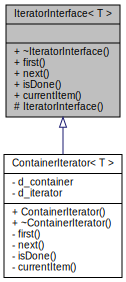
\includegraphics[width=198pt]{class_iterator_interface__inherit__graph}
\end{center}
\end{figure}
\subsection*{Public Member Functions}
\begin{DoxyCompactItemize}
\item 
virtual \hyperlink{class_iterator_interface_a4aa5b5b0bf88e8fabcaa655fdd52b6cf}{$\sim$IteratorInterface} ()
\item 
virtual void \hyperlink{class_iterator_interface_a0376168477377aad0442f89bb0f28d2b}{first} ()=0
\item 
virtual void \hyperlink{class_iterator_interface_aec2d9693127c9909bc6fc2732bfe5bac}{next} ()=0
\item 
virtual bool \hyperlink{class_iterator_interface_a8b405842b32836c6b3587bf26f09a0d4}{isDone} ()=0
\item 
virtual T \hyperlink{class_iterator_interface_a1724076d202e22aefd13325c06a91033}{currentItem} ()=0
\end{DoxyCompactItemize}
\subsection*{Protected Member Functions}
\begin{DoxyCompactItemize}
\item 
\hyperlink{class_iterator_interface_a772e4932f8d5b3c541c6eb8494183ddf}{IteratorInterface} ()
\end{DoxyCompactItemize}


\subsection{Detailed Description}
\subsubsection*{template$<$typename T$>$class IteratorInterface$<$ T $>$}

class \hyperlink{class_iterator_interface}{IteratorInterface} -\/ 

Definition at line 4 of file IteratorInterface.h.



\subsection{Constructor \& Destructor Documentation}
\hypertarget{class_iterator_interface_a4aa5b5b0bf88e8fabcaa655fdd52b6cf}{
\index{IteratorInterface@{IteratorInterface}!$\sim$IteratorInterface@{$\sim$IteratorInterface}}
\index{$\sim$IteratorInterface@{$\sim$IteratorInterface}!IteratorInterface@{IteratorInterface}}
\subsubsection[{$\sim$IteratorInterface}]{\setlength{\rightskip}{0pt plus 5cm}template$<$typename T $>$ {\bf IteratorInterface}$<$ T $>$::$\sim${\bf IteratorInterface} (
\begin{DoxyParamCaption}
{}
\end{DoxyParamCaption}
)\hspace{0.3cm}{\ttfamily  \mbox{[}virtual\mbox{]}}}}
\label{class_iterator_interface_a4aa5b5b0bf88e8fabcaa655fdd52b6cf}


Definition at line 10 of file IteratorInterface.cpp.


\begin{DoxyCode}
  {
  }
\end{DoxyCode}
\hypertarget{class_iterator_interface_a772e4932f8d5b3c541c6eb8494183ddf}{
\index{IteratorInterface@{IteratorInterface}!IteratorInterface@{IteratorInterface}}
\index{IteratorInterface@{IteratorInterface}!IteratorInterface@{IteratorInterface}}
\subsubsection[{IteratorInterface}]{\setlength{\rightskip}{0pt plus 5cm}template$<$typename T $>$ {\bf IteratorInterface}$<$ T $>$::{\bf IteratorInterface} (
\begin{DoxyParamCaption}
{}
\end{DoxyParamCaption}
)\hspace{0.3cm}{\ttfamily  \mbox{[}protected\mbox{]}}}}
\label{class_iterator_interface_a772e4932f8d5b3c541c6eb8494183ddf}


Definition at line 4 of file IteratorInterface.cpp.


\begin{DoxyCode}
  {
  }
\end{DoxyCode}


\subsection{Member Function Documentation}
\hypertarget{class_iterator_interface_a1724076d202e22aefd13325c06a91033}{
\index{IteratorInterface@{IteratorInterface}!currentItem@{currentItem}}
\index{currentItem@{currentItem}!IteratorInterface@{IteratorInterface}}
\subsubsection[{currentItem}]{\setlength{\rightskip}{0pt plus 5cm}template$<$typename T $>$ virtual T {\bf IteratorInterface}$<$ T $>$::currentItem (
\begin{DoxyParamCaption}
{}
\end{DoxyParamCaption}
)\hspace{0.3cm}{\ttfamily  \mbox{[}pure virtual\mbox{]}}}}
\label{class_iterator_interface_a1724076d202e22aefd13325c06a91033}


Implemented in \hyperlink{class_container_iterator_a088e991e5eade5740290342a49d71467}{ContainerIterator$<$ T $>$}.

\hypertarget{class_iterator_interface_a0376168477377aad0442f89bb0f28d2b}{
\index{IteratorInterface@{IteratorInterface}!first@{first}}
\index{first@{first}!IteratorInterface@{IteratorInterface}}
\subsubsection[{first}]{\setlength{\rightskip}{0pt plus 5cm}template$<$typename T $>$ virtual void {\bf IteratorInterface}$<$ T $>$::first (
\begin{DoxyParamCaption}
{}
\end{DoxyParamCaption}
)\hspace{0.3cm}{\ttfamily  \mbox{[}pure virtual\mbox{]}}}}
\label{class_iterator_interface_a0376168477377aad0442f89bb0f28d2b}


Implemented in \hyperlink{class_container_iterator_a98924935aa2d0b5f1d3bdbb8b3bc0a69}{ContainerIterator$<$ T $>$}.

\hypertarget{class_iterator_interface_a8b405842b32836c6b3587bf26f09a0d4}{
\index{IteratorInterface@{IteratorInterface}!isDone@{isDone}}
\index{isDone@{isDone}!IteratorInterface@{IteratorInterface}}
\subsubsection[{isDone}]{\setlength{\rightskip}{0pt plus 5cm}template$<$typename T $>$ virtual bool {\bf IteratorInterface}$<$ T $>$::isDone (
\begin{DoxyParamCaption}
{}
\end{DoxyParamCaption}
)\hspace{0.3cm}{\ttfamily  \mbox{[}pure virtual\mbox{]}}}}
\label{class_iterator_interface_a8b405842b32836c6b3587bf26f09a0d4}


Implemented in \hyperlink{class_container_iterator_a533dcd7d4c59663c0ae99f67f4b5e9c6}{ContainerIterator$<$ T $>$}.

\hypertarget{class_iterator_interface_aec2d9693127c9909bc6fc2732bfe5bac}{
\index{IteratorInterface@{IteratorInterface}!next@{next}}
\index{next@{next}!IteratorInterface@{IteratorInterface}}
\subsubsection[{next}]{\setlength{\rightskip}{0pt plus 5cm}template$<$typename T $>$ virtual void {\bf IteratorInterface}$<$ T $>$::next (
\begin{DoxyParamCaption}
{}
\end{DoxyParamCaption}
)\hspace{0.3cm}{\ttfamily  \mbox{[}pure virtual\mbox{]}}}}
\label{class_iterator_interface_aec2d9693127c9909bc6fc2732bfe5bac}


Implemented in \hyperlink{class_container_iterator_ae9996be7cbe4ada65c214372da509049}{ContainerIterator$<$ T $>$}.



The documentation for this class was generated from the following files:\begin{DoxyCompactItemize}
\item 
pkg/AMORE/src/dia/\hyperlink{_iterator_interface_8h}{IteratorInterface.h}\item 
pkg/AMORE/src/\hyperlink{_iterator_interface_8cpp}{IteratorInterface.cpp}\end{DoxyCompactItemize}

\hypertarget{class_layer}{
\section{Layer Class Reference}
\label{class_layer}\index{Layer@{Layer}}
}


class \hyperlink{class_layer}{Layer} -\/  




{\ttfamily \#include $<$Layer.h$>$}



Collaboration diagram for Layer:
\nopagebreak
\begin{figure}[H]
\begin{center}
\leavevmode
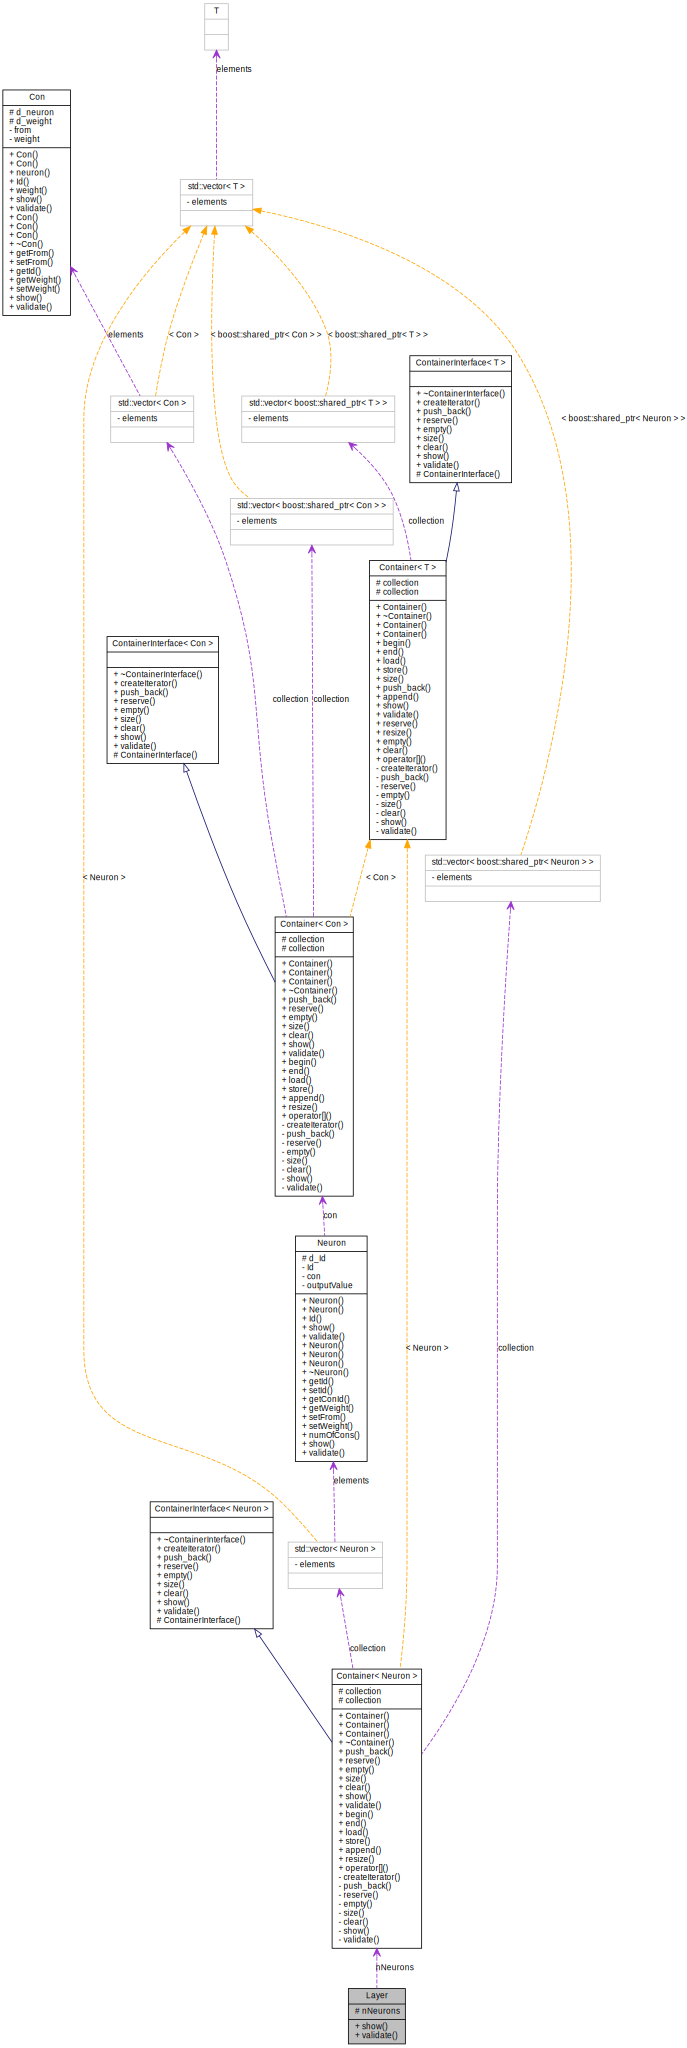
\includegraphics[height=600pt]{class_layer__coll__graph}
\end{center}
\end{figure}
\subsection*{Public Member Functions}
\begin{DoxyCompactItemize}
\item 
void \hyperlink{class_layer_a480472458a4a6c293c11b34e80a41129}{show} ()
\item 
bool \hyperlink{class_layer_a59a098968d5a8aaaf70a873429e34ce9}{validate} ()
\end{DoxyCompactItemize}
\subsection*{Protected Attributes}
\begin{DoxyCompactItemize}
\item 
\hyperlink{class_container}{Container}$<$ \hyperlink{class_neuron}{Neuron} $>$ \hyperlink{class_layer_ac573cbb1730f10aee938edb0a8a1c382}{nNeurons}
\end{DoxyCompactItemize}


\subsection{Detailed Description}
class \hyperlink{class_layer}{Layer} -\/ 

Definition at line 3 of file Layer.h.



\subsection{Member Function Documentation}
\hypertarget{class_layer_a480472458a4a6c293c11b34e80a41129}{
\index{Layer@{Layer}!show@{show}}
\index{show@{show}!Layer@{Layer}}
\subsubsection[{show}]{\setlength{\rightskip}{0pt plus 5cm}void Layer::show (
\begin{DoxyParamCaption}
{}
\end{DoxyParamCaption}
)}}
\label{class_layer_a480472458a4a6c293c11b34e80a41129}
\hypertarget{class_layer_a59a098968d5a8aaaf70a873429e34ce9}{
\index{Layer@{Layer}!validate@{validate}}
\index{validate@{validate}!Layer@{Layer}}
\subsubsection[{validate}]{\setlength{\rightskip}{0pt plus 5cm}bool Layer::validate (
\begin{DoxyParamCaption}
{}
\end{DoxyParamCaption}
)}}
\label{class_layer_a59a098968d5a8aaaf70a873429e34ce9}


\subsection{Member Data Documentation}
\hypertarget{class_layer_ac573cbb1730f10aee938edb0a8a1c382}{
\index{Layer@{Layer}!nNeurons@{nNeurons}}
\index{nNeurons@{nNeurons}!Layer@{Layer}}
\subsubsection[{nNeurons}]{\setlength{\rightskip}{0pt plus 5cm}{\bf Container}$<${\bf Neuron}$>$ {\bf Layer::nNeurons}\hspace{0.3cm}{\ttfamily  \mbox{[}protected\mbox{]}}}}
\label{class_layer_ac573cbb1730f10aee938edb0a8a1c382}


Definition at line 6 of file Layer.h.



The documentation for this class was generated from the following file:\begin{DoxyCompactItemize}
\item 
pkg/AMORE/src/dia/\hyperlink{_layer_8h}{Layer.h}\end{DoxyCompactItemize}

\hypertarget{class_m_l_player}{
\section{MLPlayer Class Reference}
\label{class_m_l_player}\index{MLPlayer@{MLPlayer}}
}


{\ttfamily \#include $<$MLPlayer.h$>$}



Inheritance diagram for MLPlayer:\nopagebreak
\begin{figure}[H]
\begin{center}
\leavevmode
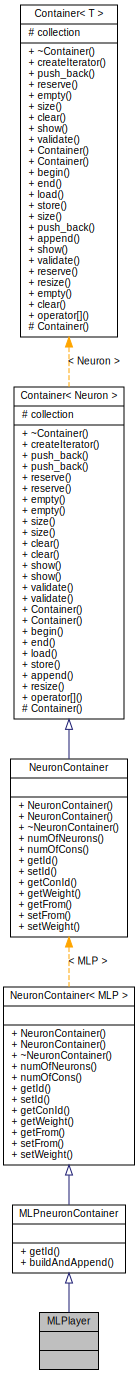
\includegraphics[height=600pt]{class_m_l_player__inherit__graph}
\end{center}
\end{figure}


Collaboration diagram for MLPlayer:\nopagebreak
\begin{figure}[H]
\begin{center}
\leavevmode
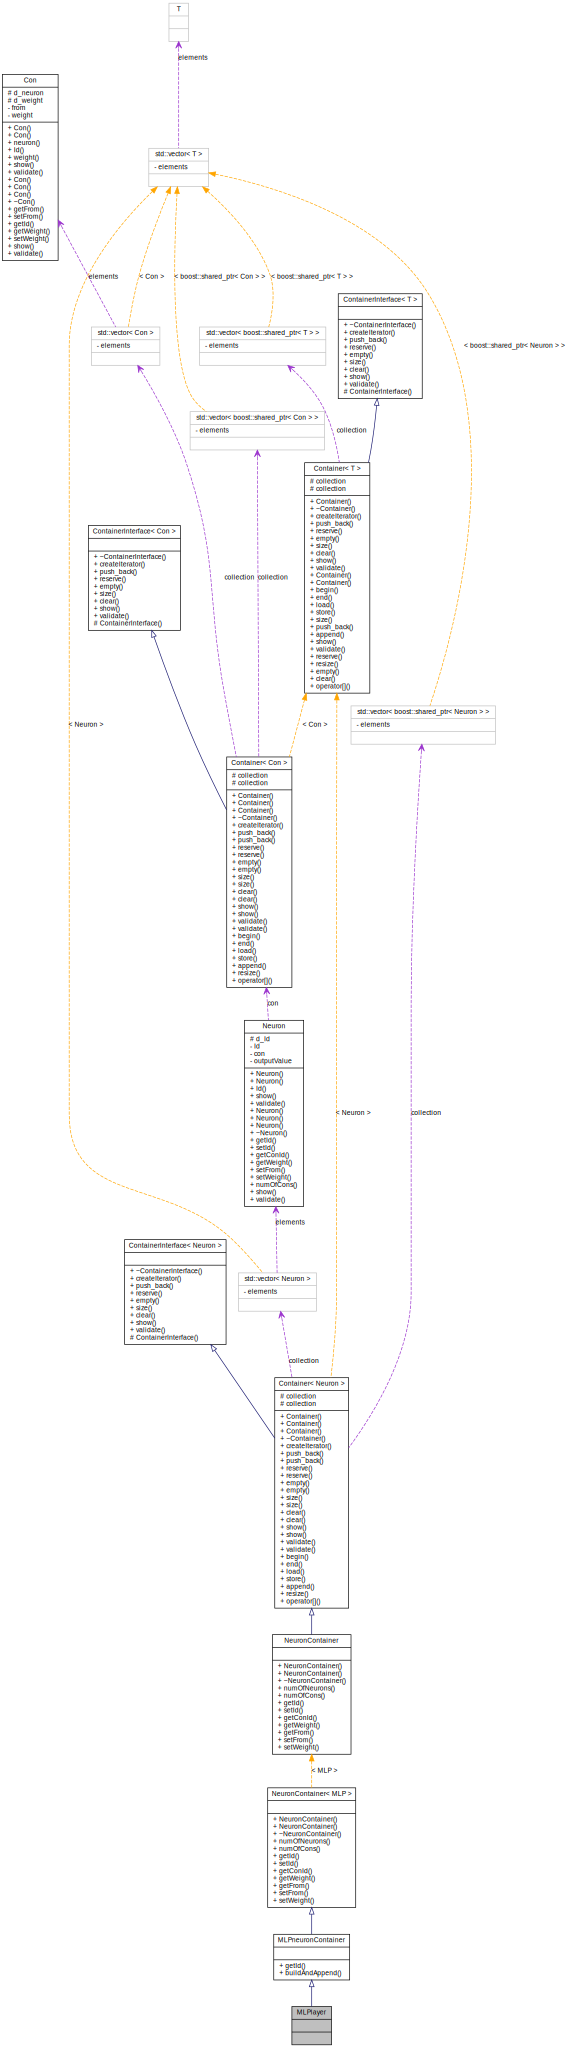
\includegraphics[height=600pt]{class_m_l_player__coll__graph}
\end{center}
\end{figure}


\subsection{Detailed Description}


Definition at line 1 of file MLPlayer.h.



The documentation for this class was generated from the following file:\begin{DoxyCompactItemize}
\item 
pkg/AMORE/src/old/\hyperlink{_m_l_player_8h}{MLPlayer.h}\end{DoxyCompactItemize}

\hypertarget{class_m_l_player_container}{
\section{MLPlayerContainer Class Reference}
\label{class_m_l_player_container}\index{MLPlayerContainer@{MLPlayerContainer}}
}


{\ttfamily \#include $<$MLPlayerContainer.h$>$}



Inheritance diagram for MLPlayerContainer:\nopagebreak
\begin{figure}[H]
\begin{center}
\leavevmode
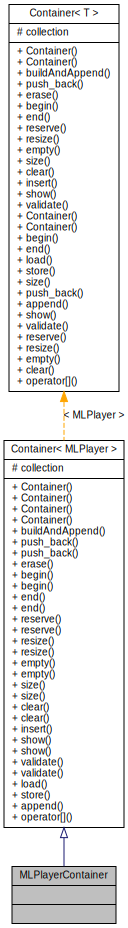
\includegraphics[height=600pt]{class_m_l_player_container__inherit__graph}
\end{center}
\end{figure}


Collaboration diagram for MLPlayerContainer:\nopagebreak
\begin{figure}[H]
\begin{center}
\leavevmode
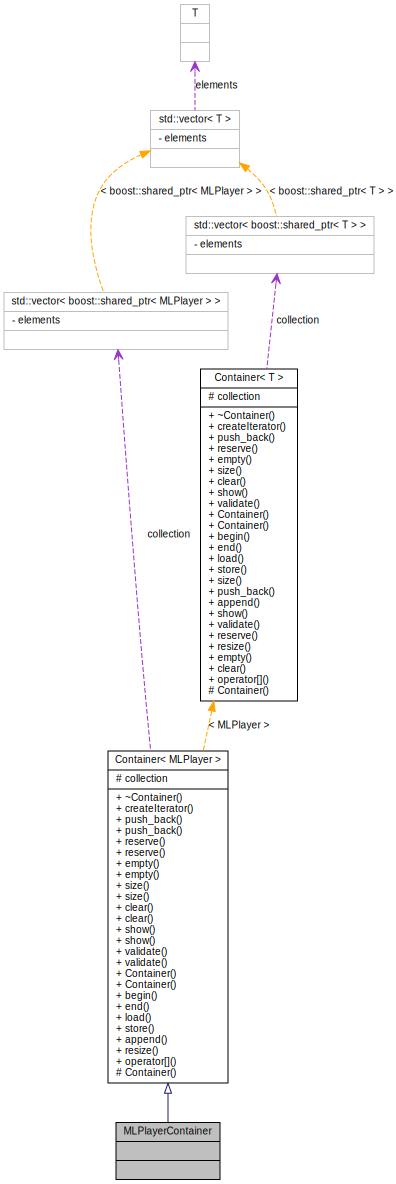
\includegraphics[height=600pt]{class_m_l_player_container__coll__graph}
\end{center}
\end{figure}


\subsection{Detailed Description}


Definition at line 1 of file MLPlayerContainer.h.



The documentation for this class was generated from the following file:\begin{DoxyCompactItemize}
\item 
pkg/AMORE/src/old/\hyperlink{_m_l_player_container_8h}{MLPlayerContainer.h}\end{DoxyCompactItemize}

\hypertarget{class_m_l_pneural_net}{
\section{MLPneuralNet Class Reference}
\label{class_m_l_pneural_net}\index{MLPneuralNet@{MLPneuralNet}}
}


class \hyperlink{class_m_l_pneural_net}{MLPneuralNet} -\/  




{\ttfamily \#include $<$MLPneuralNet.h$>$}



Inheritance diagram for MLPneuralNet:\nopagebreak
\begin{figure}[H]
\begin{center}
\leavevmode
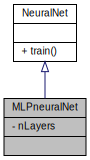
\includegraphics[width=162pt]{class_m_l_pneural_net__inherit__graph}
\end{center}
\end{figure}


Collaboration diagram for MLPneuralNet:
\nopagebreak
\begin{figure}[H]
\begin{center}
\leavevmode
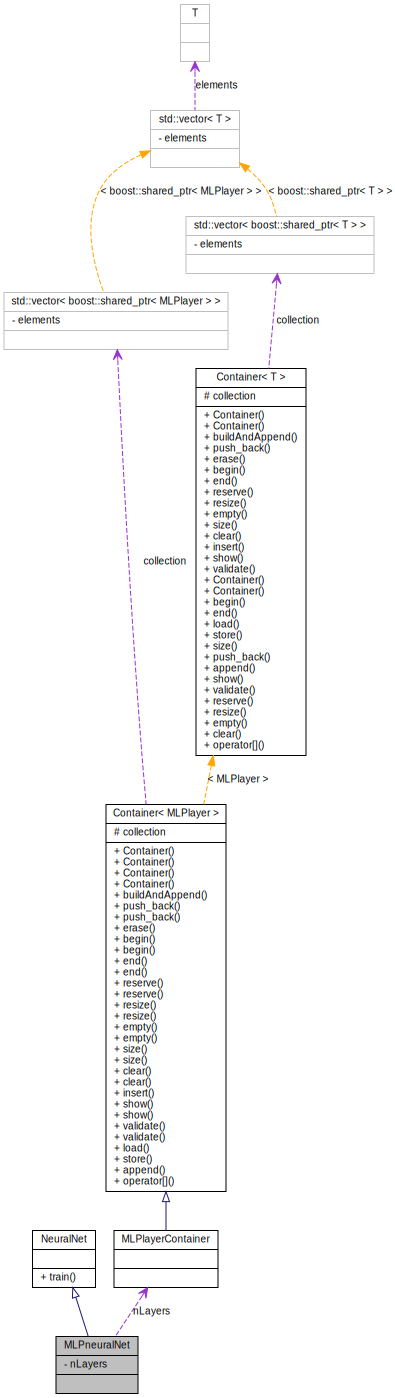
\includegraphics[height=600pt]{class_m_l_pneural_net__coll__graph}
\end{center}
\end{figure}
\subsection*{Public Member Functions}
\begin{DoxyCompactItemize}
\item 
void \hyperlink{class_m_l_pneural_net_ae92624bfac84bda339013a27db8308af}{show} ()
\item 
bool \hyperlink{class_m_l_pneural_net_ae0aae6e9c474eef1cfb1fdff98bf1360}{validate} ()
\end{DoxyCompactItemize}
\subsection*{Public Attributes}
\begin{DoxyCompactItemize}
\item 
\hyperlink{class_container}{Container}$<$ \hyperlink{class_layer}{Layer} $>$ \hyperlink{class_m_l_pneural_net_a104c89adf87a30b2cf67a456612e5125}{nLayers}
\end{DoxyCompactItemize}
\subsection*{Private Attributes}
\begin{DoxyCompactItemize}
\item 
\hyperlink{class_m_l_player_container}{MLPlayerContainer} \hyperlink{class_m_l_pneural_net_a47ac9b8f98813bf63598c78ad444d6db}{nLayers}
\end{DoxyCompactItemize}


\subsection{Detailed Description}
class \hyperlink{class_m_l_pneural_net}{MLPneuralNet} -\/ 

Definition at line 5 of file MLPneuralNet.h.



\subsection{Member Function Documentation}
\hypertarget{class_m_l_pneural_net_ae92624bfac84bda339013a27db8308af}{
\index{MLPneuralNet@{MLPneuralNet}!show@{show}}
\index{show@{show}!MLPneuralNet@{MLPneuralNet}}
\subsubsection[{show}]{\setlength{\rightskip}{0pt plus 5cm}void MLPneuralNet::show (
\begin{DoxyParamCaption}
{}
\end{DoxyParamCaption}
)}}
\label{class_m_l_pneural_net_ae92624bfac84bda339013a27db8308af}


Reimplemented from \hyperlink{class_neural_net_a633859baa979c7f10acdc99deb26c891}{NeuralNet}.

\hypertarget{class_m_l_pneural_net_ae0aae6e9c474eef1cfb1fdff98bf1360}{
\index{MLPneuralNet@{MLPneuralNet}!validate@{validate}}
\index{validate@{validate}!MLPneuralNet@{MLPneuralNet}}
\subsubsection[{validate}]{\setlength{\rightskip}{0pt plus 5cm}bool MLPneuralNet::validate (
\begin{DoxyParamCaption}
{}
\end{DoxyParamCaption}
)}}
\label{class_m_l_pneural_net_ae0aae6e9c474eef1cfb1fdff98bf1360}


Reimplemented from \hyperlink{class_neural_net_a3088aef3aa1fa865621a9609b12c948c}{NeuralNet}.



\subsection{Member Data Documentation}
\hypertarget{class_m_l_pneural_net_a104c89adf87a30b2cf67a456612e5125}{
\index{MLPneuralNet@{MLPneuralNet}!nLayers@{nLayers}}
\index{nLayers@{nLayers}!MLPneuralNet@{MLPneuralNet}}
\subsubsection[{nLayers}]{\setlength{\rightskip}{0pt plus 5cm}{\bf Container}$<${\bf Layer}$>$ {\bf MLPneuralNet::nLayers}}}
\label{class_m_l_pneural_net_a104c89adf87a30b2cf67a456612e5125}


Definition at line 8 of file MLPneuralNet.h.

\hypertarget{class_m_l_pneural_net_a47ac9b8f98813bf63598c78ad444d6db}{
\index{MLPneuralNet@{MLPneuralNet}!nLayers@{nLayers}}
\index{nLayers@{nLayers}!MLPneuralNet@{MLPneuralNet}}
\subsubsection[{nLayers}]{\setlength{\rightskip}{0pt plus 5cm}{\bf MLPlayerContainer} {\bf MLPneuralNet::nLayers}\hspace{0.3cm}{\ttfamily  \mbox{[}private\mbox{]}}}}
\label{class_m_l_pneural_net_a47ac9b8f98813bf63598c78ad444d6db}


Definition at line 2 of file MLPneuralNet.h.



The documentation for this class was generated from the following files:\begin{DoxyCompactItemize}
\item 
pkg/AMORE/src/dia/\hyperlink{dia_2_m_l_pneural_net_8h}{MLPneuralNet.h}\item 
pkg/AMORE/src/old/\hyperlink{old_2_m_l_pneural_net_8h}{MLPneuralNet.h}\end{DoxyCompactItemize}

\hypertarget{class_m_l_pneuron}{
\section{MLPneuron Class Reference}
\label{class_m_l_pneuron}\index{MLPneuron@{MLPneuron}}
}


{\ttfamily \#include $<$MLPneuron.h$>$}



Inheritance diagram for MLPneuron:
\nopagebreak
\begin{figure}[H]
\begin{center}
\leavevmode
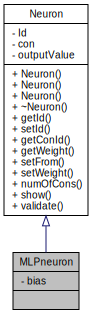
\includegraphics[width=182pt]{class_m_l_pneuron__inherit__graph}
\end{center}
\end{figure}


Collaboration diagram for MLPneuron:
\nopagebreak
\begin{figure}[H]
\begin{center}
\leavevmode
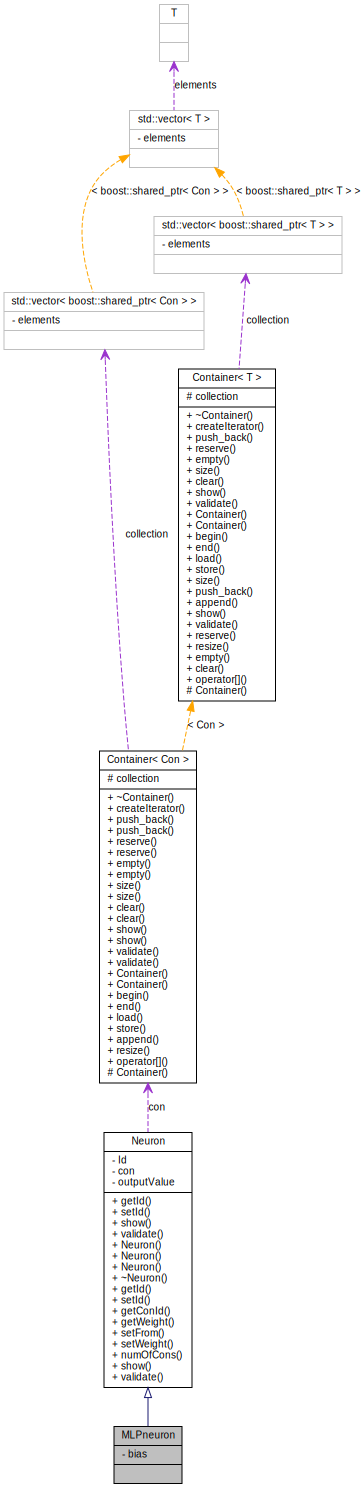
\includegraphics[height=600pt]{class_m_l_pneuron__coll__graph}
\end{center}
\end{figure}
\subsection*{Private Attributes}
\begin{DoxyCompactItemize}
\item 
int \hyperlink{class_m_l_pneuron_a6f8cb5b2fbf48db003ea8a413ffdbd8b}{bias}
\end{DoxyCompactItemize}


\subsection{Detailed Description}


Definition at line 1 of file MLPneuron.h.



\subsection{Member Data Documentation}
\hypertarget{class_m_l_pneuron_a6f8cb5b2fbf48db003ea8a413ffdbd8b}{
\index{MLPneuron@{MLPneuron}!bias@{bias}}
\index{bias@{bias}!MLPneuron@{MLPneuron}}
\subsubsection[{bias}]{\setlength{\rightskip}{0pt plus 5cm}int {\bf MLPneuron::bias}\hspace{0.3cm}{\ttfamily  \mbox{[}private\mbox{]}}}}
\label{class_m_l_pneuron_a6f8cb5b2fbf48db003ea8a413ffdbd8b}


Definition at line 2 of file MLPneuron.h.



The documentation for this class was generated from the following file:\begin{DoxyCompactItemize}
\item 
pkg/AMORE/src/old/\hyperlink{_m_l_pneuron_8h}{MLPneuron.h}\end{DoxyCompactItemize}

\hypertarget{class_m_l_pneuron_container}{
\section{MLPneuronContainer Class Reference}
\label{class_m_l_pneuron_container}\index{MLPneuronContainer@{MLPneuronContainer}}
}


A vector of connections.  




{\ttfamily \#include $<$MLPneuronContainer.h$>$}



Inheritance diagram for MLPneuronContainer:
\nopagebreak
\begin{figure}[H]
\begin{center}
\leavevmode
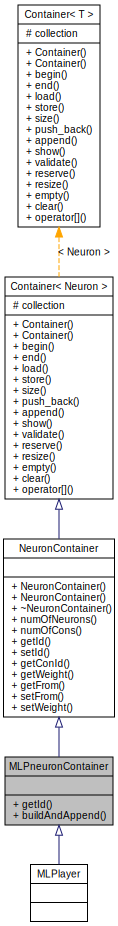
\includegraphics[height=600pt]{class_m_l_pneuron_container__inherit__graph}
\end{center}
\end{figure}


Collaboration diagram for MLPneuronContainer:
\nopagebreak
\begin{figure}[H]
\begin{center}
\leavevmode
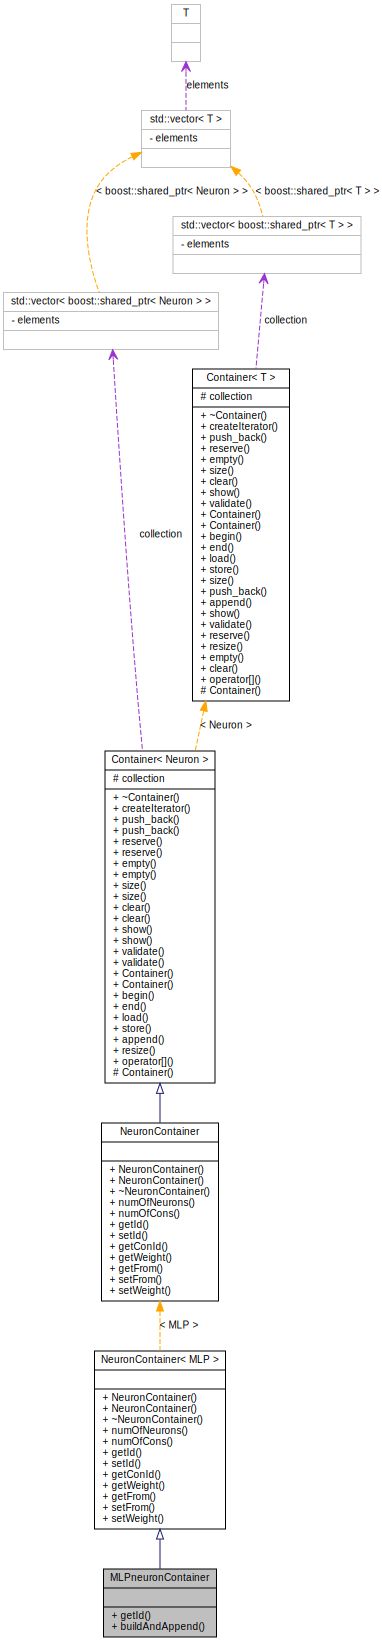
\includegraphics[height=600pt]{class_m_l_pneuron_container__coll__graph}
\end{center}
\end{figure}
\subsection*{Public Member Functions}
\begin{DoxyCompactItemize}
\item 
std::vector$<$ int $>$ \hyperlink{class_m_l_pneuron_container_a91f7def6fa9ee973b95f673642b2c586}{getId} ()
\item 
bool \hyperlink{class_m_l_pneuron_container_a98391f4cc53bb177c7abd0ff023f3cb0}{buildAndAppend} (std::vector$<$ int $>$ IDS, std::vector$<$ int $>$ BIAS, \hyperlink{class_con_container}{ConContainer} VC)
\end{DoxyCompactItemize}


\subsection{Detailed Description}
A vector of connections. 

The \hyperlink{class_con_container}{ConContainer} class provides a simple class for a vector of connections. It's named after the R equivalent Reference Class. 

Definition at line 16 of file MLPneuronContainer.h.



\subsection{Member Function Documentation}
\hypertarget{class_m_l_pneuron_container_a98391f4cc53bb177c7abd0ff023f3cb0}{
\index{MLPneuronContainer@{MLPneuronContainer}!buildAndAppend@{buildAndAppend}}
\index{buildAndAppend@{buildAndAppend}!MLPneuronContainer@{MLPneuronContainer}}
\subsubsection[{buildAndAppend}]{\setlength{\rightskip}{0pt plus 5cm}bool MLPneuronContainer::buildAndAppend (
\begin{DoxyParamCaption}
\item[{std::vector$<$ int $>$}]{IDS, }
\item[{std::vector$<$ int $>$}]{BIAS, }
\item[{{\bf ConContainer}}]{VC}
\end{DoxyParamCaption}
)}}
\label{class_m_l_pneuron_container_a98391f4cc53bb177c7abd0ff023f3cb0}
\hypertarget{class_m_l_pneuron_container_a91f7def6fa9ee973b95f673642b2c586}{
\index{MLPneuronContainer@{MLPneuronContainer}!getId@{getId}}
\index{getId@{getId}!MLPneuronContainer@{MLPneuronContainer}}
\subsubsection[{getId}]{\setlength{\rightskip}{0pt plus 5cm}std::vector$<$int$>$ MLPneuronContainer::getId (
\begin{DoxyParamCaption}
{}
\end{DoxyParamCaption}
)}}
\label{class_m_l_pneuron_container_a91f7def6fa9ee973b95f673642b2c586}


Reimplemented from \hyperlink{class_neuron_container_a2ca2c86b3a0517636b1a0b3debfd158d}{NeuronContainer$<$ MLP $>$}.



The documentation for this class was generated from the following file:\begin{DoxyCompactItemize}
\item 
pkg/AMORE/src/old/\hyperlink{_m_l_pneuron_container_8h}{MLPneuronContainer.h}\end{DoxyCompactItemize}

\hypertarget{class_neural_net}{
\section{NeuralNet Class Reference}
\label{class_neural_net}\index{NeuralNet@{NeuralNet}}
}


{\ttfamily \#include $<$NeuralNet.h$>$}



Inheritance diagram for NeuralNet:
\nopagebreak
\begin{figure}[H]
\begin{center}
\leavevmode
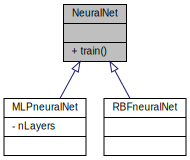
\includegraphics[width=262pt]{class_neural_net__inherit__graph}
\end{center}
\end{figure}
\subsection*{Public Member Functions}
\begin{DoxyCompactItemize}
\item 
virtual void \hyperlink{class_neural_net_a3cbf78358ad16a2e86fc7a2db746f017}{train} ()=0
\end{DoxyCompactItemize}


\subsection{Detailed Description}


Definition at line 1 of file NeuralNet.h.



\subsection{Member Function Documentation}
\hypertarget{class_neural_net_a3cbf78358ad16a2e86fc7a2db746f017}{
\index{NeuralNet@{NeuralNet}!train@{train}}
\index{train@{train}!NeuralNet@{NeuralNet}}
\subsubsection[{train}]{\setlength{\rightskip}{0pt plus 5cm}virtual void NeuralNet::train (
\begin{DoxyParamCaption}
{}
\end{DoxyParamCaption}
)\hspace{0.3cm}{\ttfamily  \mbox{[}pure virtual\mbox{]}}}}
\label{class_neural_net_a3cbf78358ad16a2e86fc7a2db746f017}


The documentation for this class was generated from the following file:\begin{DoxyCompactItemize}
\item 
pkg/AMORE/src/\hyperlink{_neural_net_8h}{NeuralNet.h}\end{DoxyCompactItemize}

\hypertarget{class_neuron}{
\section{Neuron Class Reference}
\label{class_neuron}\index{Neuron@{Neuron}}
}


A class to handle the information contained in a general \hyperlink{class_neuron}{Neuron}.  




{\ttfamily \#include $<$Neuron.h$>$}



Collaboration diagram for Neuron:
\nopagebreak
\begin{figure}[H]
\begin{center}
\leavevmode
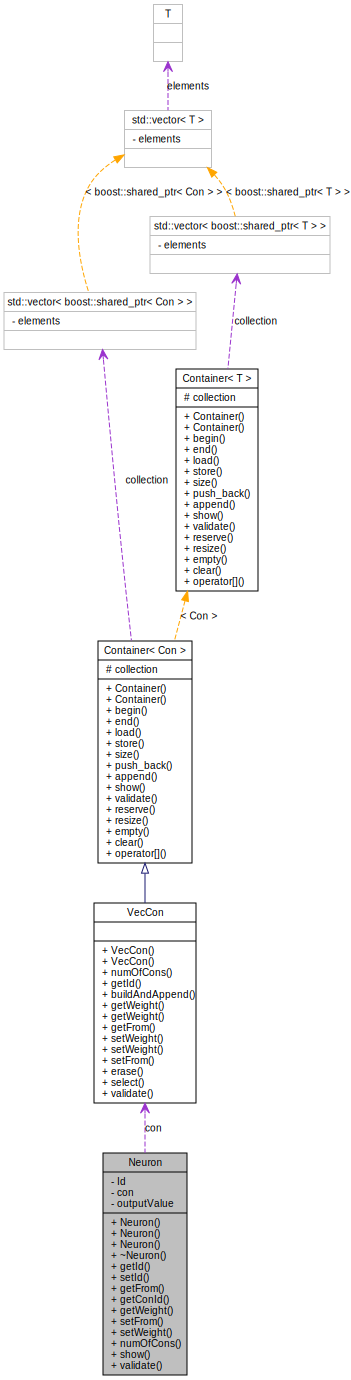
\includegraphics[height=600pt]{class_neuron__coll__graph}
\end{center}
\end{figure}
\subsection*{Public Member Functions}
\begin{DoxyCompactItemize}
\item 
\hyperlink{class_neuron_a823487d01615fadb8ac19a2768dd9d96}{Neuron} ()
\item 
\hyperlink{class_neuron_a05698a11ac18b6cee34d18f63681ddcc}{Neuron} (int \hyperlink{class_neuron_a72bb327a7c5c865e6748a4e074ce0680}{Id})
\item 
\hyperlink{class_neuron_af6ba81347cc25d4d5d256dba2c4e441a}{Neuron} (int \hyperlink{class_neuron_a72bb327a7c5c865e6748a4e074ce0680}{Id}, \hyperlink{class_vec_con}{VecCon} \hyperlink{class_con}{Con})
\item 
\hyperlink{class_neuron_a94a250ce7e167760e593979b899745b1}{$\sim$Neuron} ()
\item 
int \hyperlink{class_neuron_ad9211d55ea50ad6dfbd2676b9e2335e4}{getId} ()
\item 
void \hyperlink{class_neuron_a6eb17a0d297b8c65170911aff37ba968}{setId} (int \hyperlink{class_neuron_a72bb327a7c5c865e6748a4e074ce0680}{Id})
\item 
std::vector$<$ \hyperlink{_a_m_o_r_e_8h_ac1ea936c2c7728eb382278131652fef4}{NeuronPtr} $>$ \hyperlink{class_neuron_a66e3800037d2789a8fe7b73996c14f84}{getFrom} ()
\item 
std::vector$<$ int $>$ \hyperlink{class_neuron_aac7d538b4a5087f730ba80f19852bced}{getConId} ()
\item 
std::vector$<$ double $>$ \hyperlink{class_neuron_a3349c0a2053e35afa5b7036bb816f8c6}{getWeight} ()
\item 
bool \hyperlink{class_neuron_ace0e92348f8a5604f25a3cfc07f38ec8}{setFrom} (std::vector$<$ \hyperlink{_a_m_o_r_e_8h_ac1ea936c2c7728eb382278131652fef4}{NeuronPtr} $>$ vFrom)
\item 
bool \hyperlink{class_neuron_ab067bfe507f5386eccc860d4ad2d0bca}{setWeight} (std::vector$<$ double $>$ vWeight)
\item 
int \hyperlink{class_neuron_ae447dce39ed04581609a83d742b585d1}{numOfCons} ()
\item 
bool \hyperlink{class_neuron_a255c3597520c730d798218f7174eff1b}{show} ()
\item 
bool \hyperlink{class_neuron_a95327aa80a9ec949491f214a0c159b5a}{validate} ()
\end{DoxyCompactItemize}
\subsection*{Private Attributes}
\begin{DoxyCompactItemize}
\item 
int \hyperlink{class_neuron_a72bb327a7c5c865e6748a4e074ce0680}{Id}
\begin{DoxyCompactList}\small\item\em An integer variable with the \hyperlink{class_neuron}{Neuron} Id. \end{DoxyCompactList}\item 
\hyperlink{class_vec_con}{VecCon} \hyperlink{class_neuron_a1451f2424a8f9e46ca643d03ff98a616}{con}
\begin{DoxyCompactList}\small\item\em A vector of input connections. \end{DoxyCompactList}\item 
double \hyperlink{class_neuron_ada029047646c36e525a6a1b77cafc03c}{outputValue}
\end{DoxyCompactItemize}


\subsection{Detailed Description}
A class to handle the information contained in a general \hyperlink{class_neuron}{Neuron}. 

A general class for neurons. The MLPneuron and RBFneuron classes will specialize this general class 

Definition at line 16 of file Neuron.h.



\subsection{Constructor \& Destructor Documentation}
\hypertarget{class_neuron_a823487d01615fadb8ac19a2768dd9d96}{
\index{Neuron@{Neuron}!Neuron@{Neuron}}
\index{Neuron@{Neuron}!Neuron@{Neuron}}
\subsubsection[{Neuron}]{\setlength{\rightskip}{0pt plus 5cm}Neuron::Neuron (
\begin{DoxyParamCaption}
{}
\end{DoxyParamCaption}
)}}
\label{class_neuron_a823487d01615fadb8ac19a2768dd9d96}


Definition at line 12 of file Neuron.cpp.


\begin{DoxyCode}
: Id(NA_INTEGER), con() {};
\end{DoxyCode}
\hypertarget{class_neuron_a05698a11ac18b6cee34d18f63681ddcc}{
\index{Neuron@{Neuron}!Neuron@{Neuron}}
\index{Neuron@{Neuron}!Neuron@{Neuron}}
\subsubsection[{Neuron}]{\setlength{\rightskip}{0pt plus 5cm}Neuron::Neuron (
\begin{DoxyParamCaption}
\item[{int}]{Id}
\end{DoxyParamCaption}
)}}
\label{class_neuron_a05698a11ac18b6cee34d18f63681ddcc}


Definition at line 13 of file Neuron.cpp.


\begin{DoxyCode}
: Id(Id), outputValue(0.0) {};
\end{DoxyCode}
\hypertarget{class_neuron_af6ba81347cc25d4d5d256dba2c4e441a}{
\index{Neuron@{Neuron}!Neuron@{Neuron}}
\index{Neuron@{Neuron}!Neuron@{Neuron}}
\subsubsection[{Neuron}]{\setlength{\rightskip}{0pt plus 5cm}Neuron::Neuron (
\begin{DoxyParamCaption}
\item[{int}]{Id, }
\item[{{\bf VecCon}}]{Con}
\end{DoxyParamCaption}
)}}
\label{class_neuron_af6ba81347cc25d4d5d256dba2c4e441a}


Definition at line 14 of file Neuron.cpp.


\begin{DoxyCode}
: Id(Id), con(con), outputValue(0.0) {} ;
\end{DoxyCode}
\hypertarget{class_neuron_a94a250ce7e167760e593979b899745b1}{
\index{Neuron@{Neuron}!$\sim$Neuron@{$\sim$Neuron}}
\index{$\sim$Neuron@{$\sim$Neuron}!Neuron@{Neuron}}
\subsubsection[{$\sim$Neuron}]{\setlength{\rightskip}{0pt plus 5cm}Neuron::$\sim$Neuron (
\begin{DoxyParamCaption}
{}
\end{DoxyParamCaption}
)}}
\label{class_neuron_a94a250ce7e167760e593979b899745b1}


Definition at line 15 of file Neuron.cpp.


\begin{DoxyCode}
{};
\end{DoxyCode}


\subsection{Member Function Documentation}
\hypertarget{class_neuron_aac7d538b4a5087f730ba80f19852bced}{
\index{Neuron@{Neuron}!getConId@{getConId}}
\index{getConId@{getConId}!Neuron@{Neuron}}
\subsubsection[{getConId}]{\setlength{\rightskip}{0pt plus 5cm}std::vector$<$ int $>$ Neuron::getConId (
\begin{DoxyParamCaption}
{}
\end{DoxyParamCaption}
)}}
\label{class_neuron_aac7d538b4a5087f730ba80f19852bced}


Definition at line 32 of file Neuron.cpp.



References con, and VecCon::getId().


\begin{DoxyCode}
                                  {
        return con.getId();
}
\end{DoxyCode}


Here is the call graph for this function:
\nopagebreak
\begin{figure}[H]
\begin{center}
\leavevmode
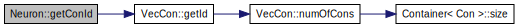
\includegraphics[width=400pt]{class_neuron_aac7d538b4a5087f730ba80f19852bced_cgraph}
\end{center}
\end{figure}


\hypertarget{class_neuron_a66e3800037d2789a8fe7b73996c14f84}{
\index{Neuron@{Neuron}!getFrom@{getFrom}}
\index{getFrom@{getFrom}!Neuron@{Neuron}}
\subsubsection[{getFrom}]{\setlength{\rightskip}{0pt plus 5cm}std::vector$<$ {\bf NeuronPtr} $>$ Neuron::getFrom (
\begin{DoxyParamCaption}
{}
\end{DoxyParamCaption}
)}}
\label{class_neuron_a66e3800037d2789a8fe7b73996c14f84}


Definition at line 27 of file Neuron.cpp.



References con, and VecCon::getFrom().


\begin{DoxyCode}
                                                  {
        return con.getFrom();
}
\end{DoxyCode}


Here is the call graph for this function:
\nopagebreak
\begin{figure}[H]
\begin{center}
\leavevmode
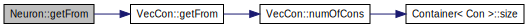
\includegraphics[width=400pt]{class_neuron_a66e3800037d2789a8fe7b73996c14f84_cgraph}
\end{center}
\end{figure}


\hypertarget{class_neuron_ad9211d55ea50ad6dfbd2676b9e2335e4}{
\index{Neuron@{Neuron}!getId@{getId}}
\index{getId@{getId}!Neuron@{Neuron}}
\subsubsection[{getId}]{\setlength{\rightskip}{0pt plus 5cm}int Neuron::getId (
\begin{DoxyParamCaption}
{}
\end{DoxyParamCaption}
)}}
\label{class_neuron_ad9211d55ea50ad6dfbd2676b9e2335e4}


Definition at line 18 of file Neuron.cpp.



References Id.



Referenced by show(), and validate().


\begin{DoxyCode}
                  {
        return Id;
}
\end{DoxyCode}


Here is the caller graph for this function:\nopagebreak
\begin{figure}[H]
\begin{center}
\leavevmode
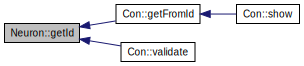
\includegraphics[width=280pt]{class_neuron_ad9211d55ea50ad6dfbd2676b9e2335e4_icgraph}
\end{center}
\end{figure}


\hypertarget{class_neuron_a3349c0a2053e35afa5b7036bb816f8c6}{
\index{Neuron@{Neuron}!getWeight@{getWeight}}
\index{getWeight@{getWeight}!Neuron@{Neuron}}
\subsubsection[{getWeight}]{\setlength{\rightskip}{0pt plus 5cm}std::vector$<$ double $>$ Neuron::getWeight (
\begin{DoxyParamCaption}
{}
\end{DoxyParamCaption}
)}}
\label{class_neuron_a3349c0a2053e35afa5b7036bb816f8c6}


Definition at line 37 of file Neuron.cpp.



References con, and VecCon::getWeight().


\begin{DoxyCode}
                                          {
        return con.getWeight();
}
\end{DoxyCode}


Here is the call graph for this function:
\nopagebreak
\begin{figure}[H]
\begin{center}
\leavevmode
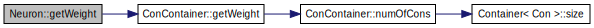
\includegraphics[width=400pt]{class_neuron_a3349c0a2053e35afa5b7036bb816f8c6_cgraph}
\end{center}
\end{figure}


\hypertarget{class_neuron_ae447dce39ed04581609a83d742b585d1}{
\index{Neuron@{Neuron}!numOfCons@{numOfCons}}
\index{numOfCons@{numOfCons}!Neuron@{Neuron}}
\subsubsection[{numOfCons}]{\setlength{\rightskip}{0pt plus 5cm}int Neuron::numOfCons (
\begin{DoxyParamCaption}
{}
\end{DoxyParamCaption}
)}}
\label{class_neuron_ae447dce39ed04581609a83d742b585d1}


Definition at line 51 of file Neuron.cpp.



References con, and VecCon::numOfCons().



Referenced by show().


\begin{DoxyCode}
                          {
        return con.numOfCons();
}
\end{DoxyCode}


Here is the call graph for this function:
\nopagebreak
\begin{figure}[H]
\begin{center}
\leavevmode
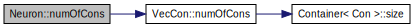
\includegraphics[width=400pt]{class_neuron_ae447dce39ed04581609a83d742b585d1_cgraph}
\end{center}
\end{figure}




Here is the caller graph for this function:
\nopagebreak
\begin{figure}[H]
\begin{center}
\leavevmode
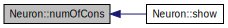
\includegraphics[width=300pt]{class_neuron_ae447dce39ed04581609a83d742b585d1_icgraph}
\end{center}
\end{figure}


\hypertarget{class_neuron_ace0e92348f8a5604f25a3cfc07f38ec8}{
\index{Neuron@{Neuron}!setFrom@{setFrom}}
\index{setFrom@{setFrom}!Neuron@{Neuron}}
\subsubsection[{setFrom}]{\setlength{\rightskip}{0pt plus 5cm}bool Neuron::setFrom (
\begin{DoxyParamCaption}
\item[{std::vector$<$ {\bf NeuronPtr} $>$}]{vFrom}
\end{DoxyParamCaption}
)}}
\label{class_neuron_ace0e92348f8a5604f25a3cfc07f38ec8}


Definition at line 42 of file Neuron.cpp.



References con, and VecCon::setFrom().


\begin{DoxyCode}
                                                            {
        con.setFrom(vFrom);
}
\end{DoxyCode}


Here is the call graph for this function:
\nopagebreak
\begin{figure}[H]
\begin{center}
\leavevmode
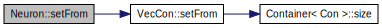
\includegraphics[width=400pt]{class_neuron_ace0e92348f8a5604f25a3cfc07f38ec8_cgraph}
\end{center}
\end{figure}


\hypertarget{class_neuron_a6eb17a0d297b8c65170911aff37ba968}{
\index{Neuron@{Neuron}!setId@{setId}}
\index{setId@{setId}!Neuron@{Neuron}}
\subsubsection[{setId}]{\setlength{\rightskip}{0pt plus 5cm}void Neuron::setId (
\begin{DoxyParamCaption}
\item[{int}]{Id}
\end{DoxyParamCaption}
)}}
\label{class_neuron_a6eb17a0d297b8c65170911aff37ba968}


Definition at line 22 of file Neuron.cpp.



References Id.


\begin{DoxyCode}
                         {
        Id=id;
}
\end{DoxyCode}
\hypertarget{class_neuron_ab067bfe507f5386eccc860d4ad2d0bca}{
\index{Neuron@{Neuron}!setWeight@{setWeight}}
\index{setWeight@{setWeight}!Neuron@{Neuron}}
\subsubsection[{setWeight}]{\setlength{\rightskip}{0pt plus 5cm}bool Neuron::setWeight (
\begin{DoxyParamCaption}
\item[{std::vector$<$ double $>$}]{vWeight}
\end{DoxyParamCaption}
)}}
\label{class_neuron_ab067bfe507f5386eccc860d4ad2d0bca}


Definition at line 47 of file Neuron.cpp.



References con, and VecCon::setWeight().


\begin{DoxyCode}
                                                   {
        con.setWeight(vWeight);
}
\end{DoxyCode}


Here is the call graph for this function:
\nopagebreak
\begin{figure}[H]
\begin{center}
\leavevmode
\includegraphics[width=400pt]{class_neuron_ab067bfe507f5386eccc860d4ad2d0bca_cgraph}
\end{center}
\end{figure}


\hypertarget{class_neuron_a255c3597520c730d798218f7174eff1b}{
\index{Neuron@{Neuron}!show@{show}}
\index{show@{show}!Neuron@{Neuron}}
\subsubsection[{show}]{\setlength{\rightskip}{0pt plus 5cm}bool Neuron::show (
\begin{DoxyParamCaption}
{}
\end{DoxyParamCaption}
)}}
\label{class_neuron_a255c3597520c730d798218f7174eff1b}


Definition at line 55 of file Neuron.cpp.



References con, getId(), numOfCons(), and Container$<$ T $>$::show().


\begin{DoxyCode}
                                  {
        int id=getId();
        Rprintf("\n------------------------\n");
        if (id==NA_INTEGER) {
                Rprintf("\n Id: NA, Invalid neuron Id");
        } else {
                Rprintf("\n Id: %d", id);
        }
        Rprintf("\n------------------------\n");
        if (numOfCons()==0) {
                Rprintf("\n No connections defined");
        } else {
                con.show();
        }
        Rprintf("\n------------------------\n");
        return true;

}
\end{DoxyCode}


Here is the call graph for this function:
\nopagebreak
\begin{figure}[H]
\begin{center}
\leavevmode
\includegraphics[width=400pt]{class_neuron_a255c3597520c730d798218f7174eff1b_cgraph}
\end{center}
\end{figure}


\hypertarget{class_neuron_a95327aa80a9ec949491f214a0c159b5a}{
\index{Neuron@{Neuron}!validate@{validate}}
\index{validate@{validate}!Neuron@{Neuron}}
\subsubsection[{validate}]{\setlength{\rightskip}{0pt plus 5cm}bool Neuron::validate (
\begin{DoxyParamCaption}
{}
\end{DoxyParamCaption}
)}}
\label{class_neuron_a95327aa80a9ec949491f214a0c159b5a}


Definition at line 75 of file Neuron.cpp.



References con, getId(), and VecCon::validate().


\begin{DoxyCode}
                          {
        BEGIN_RCPP
        if (getId() == NA_INTEGER )             throw std::range_error("[C++ Neur
      on::validate]: Error, Id is NA.");
        con.validate();
        return(TRUE);
        END_RCPP

}
\end{DoxyCode}


Here is the call graph for this function:
\nopagebreak
\begin{figure}[H]
\begin{center}
\leavevmode
\includegraphics[width=400pt]{class_neuron_a95327aa80a9ec949491f214a0c159b5a_cgraph}
\end{center}
\end{figure}




\subsection{Member Data Documentation}
\hypertarget{class_neuron_a1451f2424a8f9e46ca643d03ff98a616}{
\index{Neuron@{Neuron}!con@{con}}
\index{con@{con}!Neuron@{Neuron}}
\subsubsection[{con}]{\setlength{\rightskip}{0pt plus 5cm}{\bf VecCon} {\bf Neuron::con}\hspace{0.3cm}{\ttfamily  \mbox{[}private\mbox{]}}}}
\label{class_neuron_a1451f2424a8f9e46ca643d03ff98a616}


A vector of input connections. 



Definition at line 28 of file Neuron.h.



Referenced by getConId(), getFrom(), getWeight(), numOfCons(), setFrom(), setWeight(), show(), and validate().

\hypertarget{class_neuron_a72bb327a7c5c865e6748a4e074ce0680}{
\index{Neuron@{Neuron}!Id@{Id}}
\index{Id@{Id}!Neuron@{Neuron}}
\subsubsection[{Id}]{\setlength{\rightskip}{0pt plus 5cm}int {\bf Neuron::Id}\hspace{0.3cm}{\ttfamily  \mbox{[}private\mbox{]}}}}
\label{class_neuron_a72bb327a7c5c865e6748a4e074ce0680}


An integer variable with the \hyperlink{class_neuron}{Neuron} Id. 

The \hyperlink{class_neuron}{Neuron} Id provides a name to the neuron. This value is not expected to be used neither during simulation nor training but it provides an easy reference for human readers. 

Definition at line 21 of file Neuron.h.



Referenced by getId(), and setId().

\hypertarget{class_neuron_ada029047646c36e525a6a1b77cafc03c}{
\index{Neuron@{Neuron}!outputValue@{outputValue}}
\index{outputValue@{outputValue}!Neuron@{Neuron}}
\subsubsection[{outputValue}]{\setlength{\rightskip}{0pt plus 5cm}double {\bf Neuron::outputValue}\hspace{0.3cm}{\ttfamily  \mbox{[}private\mbox{]}}}}
\label{class_neuron_ada029047646c36e525a6a1b77cafc03c}


Definition at line 29 of file Neuron.h.



The documentation for this class was generated from the following files:\begin{DoxyCompactItemize}
\item 
pkg/AMORE/src/\hyperlink{_neuron_8h}{Neuron.h}\item 
pkg/AMORE/src/\hyperlink{_neuron_8cpp}{Neuron.cpp}\end{DoxyCompactItemize}

\hypertarget{class_neuron_container}{
\section{NeuronContainer Class Reference}
\label{class_neuron_container}\index{NeuronContainer@{NeuronContainer}}
}


A vector of neurons.  




{\ttfamily \#include $<$NeuronContainer.h$>$}



Inheritance diagram for NeuronContainer:
\nopagebreak
\begin{figure}[H]
\begin{center}
\leavevmode
\includegraphics[height=600pt]{class_neuron_container__inherit__graph}
\end{center}
\end{figure}


Collaboration diagram for NeuronContainer:
\nopagebreak
\begin{figure}[H]
\begin{center}
\leavevmode
\includegraphics[height=600pt]{class_neuron_container__coll__graph}
\end{center}
\end{figure}
\subsection*{Public Types}
\begin{DoxyCompactItemize}
\item 
typedef \hyperlink{_a_m_o_r_e_8h_a36be90b8d9f454d85104cd4a44467e00}{NeuronContainer\_\-iterator} \hyperlink{class_neuron_container_abf81356adaea3bfc64aa03777e9a8def}{iterator}
\item 
typedef \hyperlink{_a_m_o_r_e_8h_af3f69a84a2f298d29ab490ec36f6d247}{NeuronContainer\_\-const\_\-iterator} \hyperlink{class_neuron_container_a41749602f05e7610da7f0f1fd59f5442}{const\_\-iterator}
\item 
typedef boost::shared\_\-ptr$<$ \hyperlink{class_neuron}{Neuron} $>$ \hyperlink{class_neuron_container_ac067345f1d27a5b04e4d9487b319ccaa}{value\_\-type}
\item 
typedef \hyperlink{class_neuron_container_ac067345f1d27a5b04e4d9487b319ccaa}{value\_\-type} const \& \hyperlink{class_neuron_container_a468ffbb00b15553f73da46dd62c91c8d}{const\_\-reference}
\end{DoxyCompactItemize}
\subsection*{Public Member Functions}
\begin{DoxyCompactItemize}
\item 
\hyperlink{class_neuron_container_a9b22029b084f7446d2dfafc2e8f89700}{NeuronContainer} ()
\item 
\hyperlink{class_neuron_container_a85e1e7946db7317179adbe359dc4ac39}{NeuronContainer} (std::vector$<$ \hyperlink{_a_m_o_r_e_8h_a1948728c64a74ecbdc50c0f0e43ecfd1}{NeuronPtr} $>$ neuronContainer)
\item 
\hyperlink{class_neuron_container_a908e984efdd9dc08b507c95b23b295dd}{$\sim$NeuronContainer} ()
\item 
int \hyperlink{class_neuron_container_a37132392f025c0358d2f47a03bb4854f}{numOfNeurons} ()
\item 
std::vector$<$ int $>$ \hyperlink{class_neuron_container_a70c5fd8e735b04c48b29cc17b77ff301}{numOfCons} ()
\item 
std::vector$<$ int $>$ \hyperlink{class_neuron_container_a2ca2c86b3a0517636b1a0b3debfd158d}{getId} ()
\item 
void \hyperlink{class_neuron_container_a17c57249055e5de605e9663384ca48ce}{setId} (std::vector$<$ int $>$ nIds)
\item 
std::vector$<$ std::vector$<$ int $>$ $>$ \hyperlink{class_neuron_container_ad3ce88ba0e1beba4b60bac38c1cd2ccd}{getConId} ()
\item 
std::vector$<$ std::vector$<$ double $>$ $>$ \hyperlink{class_neuron_container_ad11f5391b58f32b6db45f31fdc4927e7}{getWeight} ()
\item 
std::vector$<$ \hyperlink{class_neuron_container}{NeuronContainer} $>$ \hyperlink{class_neuron_container_a3a0ea5632f0dfbf3159db657d6de84db}{getFrom} ()
\item 
void \hyperlink{class_neuron_container_a058524958a0fe0dfd946d9e7f4003310}{setFrom} (std::vector$<$ \hyperlink{class_neuron_container}{NeuronContainer} $>$ neuronArray)
\item 
void \hyperlink{class_neuron_container_a54d5bfaf428ab9bc66aac79c312ab997}{setWeight} (std::vector$<$ std::vector$<$ double $>$ $>$ value)
\end{DoxyCompactItemize}


\subsection{Detailed Description}
A vector of neurons. 

The vecNeuron class provides a simple class for a vector of neurons. It's named after the R equivalent Reference Class. 

Definition at line 17 of file NeuronContainer.h.



\subsection{Member Typedef Documentation}
\hypertarget{class_neuron_container_a41749602f05e7610da7f0f1fd59f5442}{
\index{NeuronContainer@{NeuronContainer}!const\_\-iterator@{const\_\-iterator}}
\index{const\_\-iterator@{const\_\-iterator}!NeuronContainer@{NeuronContainer}}
\subsubsection[{const\_\-iterator}]{\setlength{\rightskip}{0pt plus 5cm}typedef {\bf NeuronContainer\_\-const\_\-iterator} {\bf NeuronContainer::const\_\-iterator}}}
\label{class_neuron_container_a41749602f05e7610da7f0f1fd59f5442}


Reimplemented from \hyperlink{class_container_a5eabadaffdd508cb623c955eb0af1518}{Container$<$ Neuron $>$}.



Definition at line 23 of file NeuronContainer.h.

\hypertarget{class_neuron_container_a468ffbb00b15553f73da46dd62c91c8d}{
\index{NeuronContainer@{NeuronContainer}!const\_\-reference@{const\_\-reference}}
\index{const\_\-reference@{const\_\-reference}!NeuronContainer@{NeuronContainer}}
\subsubsection[{const\_\-reference}]{\setlength{\rightskip}{0pt plus 5cm}typedef {\bf value\_\-type} const\& {\bf NeuronContainer::const\_\-reference}}}
\label{class_neuron_container_a468ffbb00b15553f73da46dd62c91c8d}


Reimplemented from \hyperlink{class_container_a9aaab0502055ee85ce5d3633fbca2675}{Container$<$ Neuron $>$}.



Definition at line 27 of file NeuronContainer.h.

\hypertarget{class_neuron_container_abf81356adaea3bfc64aa03777e9a8def}{
\index{NeuronContainer@{NeuronContainer}!iterator@{iterator}}
\index{iterator@{iterator}!NeuronContainer@{NeuronContainer}}
\subsubsection[{iterator}]{\setlength{\rightskip}{0pt plus 5cm}typedef {\bf NeuronContainer\_\-iterator} {\bf NeuronContainer::iterator}}}
\label{class_neuron_container_abf81356adaea3bfc64aa03777e9a8def}


Reimplemented from \hyperlink{class_container_afe880028d8304353129f47cd1d28c20a}{Container$<$ Neuron $>$}.



Definition at line 21 of file NeuronContainer.h.

\hypertarget{class_neuron_container_ac067345f1d27a5b04e4d9487b319ccaa}{
\index{NeuronContainer@{NeuronContainer}!value\_\-type@{value\_\-type}}
\index{value\_\-type@{value\_\-type}!NeuronContainer@{NeuronContainer}}
\subsubsection[{value\_\-type}]{\setlength{\rightskip}{0pt plus 5cm}typedef boost::shared\_\-ptr$<${\bf Neuron}$>$ {\bf NeuronContainer::value\_\-type}}}
\label{class_neuron_container_ac067345f1d27a5b04e4d9487b319ccaa}


Reimplemented from \hyperlink{class_container_aa44714b9a736d2cfd2e01a87ad1c001b}{Container$<$ Neuron $>$}.



Definition at line 25 of file NeuronContainer.h.



\subsection{Constructor \& Destructor Documentation}
\hypertarget{class_neuron_container_a9b22029b084f7446d2dfafc2e8f89700}{
\index{NeuronContainer@{NeuronContainer}!NeuronContainer@{NeuronContainer}}
\index{NeuronContainer@{NeuronContainer}!NeuronContainer@{NeuronContainer}}
\subsubsection[{NeuronContainer}]{\setlength{\rightskip}{0pt plus 5cm}NeuronContainer::NeuronContainer (
\begin{DoxyParamCaption}
{}
\end{DoxyParamCaption}
)}}
\label{class_neuron_container_a9b22029b084f7446d2dfafc2e8f89700}


Definition at line 8 of file NeuronContainer.cpp.


\begin{DoxyCode}
{
}
\end{DoxyCode}
\hypertarget{class_neuron_container_a85e1e7946db7317179adbe359dc4ac39}{
\index{NeuronContainer@{NeuronContainer}!NeuronContainer@{NeuronContainer}}
\index{NeuronContainer@{NeuronContainer}!NeuronContainer@{NeuronContainer}}
\subsubsection[{NeuronContainer}]{\setlength{\rightskip}{0pt plus 5cm}NeuronContainer::NeuronContainer (
\begin{DoxyParamCaption}
\item[{std::vector$<$ {\bf NeuronPtr} $>$}]{neuronContainer}
\end{DoxyParamCaption}
)}}
\label{class_neuron_container_a85e1e7946db7317179adbe359dc4ac39}


Definition at line 12 of file NeuronContainer.cpp.


\begin{DoxyCode}
                                                                :
  Container<Neuron> (collection)
{
}
\end{DoxyCode}
\hypertarget{class_neuron_container_a908e984efdd9dc08b507c95b23b295dd}{
\index{NeuronContainer@{NeuronContainer}!$\sim$NeuronContainer@{$\sim$NeuronContainer}}
\index{$\sim$NeuronContainer@{$\sim$NeuronContainer}!NeuronContainer@{NeuronContainer}}
\subsubsection[{$\sim$NeuronContainer}]{\setlength{\rightskip}{0pt plus 5cm}NeuronContainer::$\sim$NeuronContainer (
\begin{DoxyParamCaption}
{}
\end{DoxyParamCaption}
)}}
\label{class_neuron_container_a908e984efdd9dc08b507c95b23b295dd}


Definition at line 17 of file NeuronContainer.cpp.


\begin{DoxyCode}
{
}
\end{DoxyCode}


\subsection{Member Function Documentation}
\hypertarget{class_neuron_container_ad3ce88ba0e1beba4b60bac38c1cd2ccd}{
\index{NeuronContainer@{NeuronContainer}!getConId@{getConId}}
\index{getConId@{getConId}!NeuronContainer@{NeuronContainer}}
\subsubsection[{getConId}]{\setlength{\rightskip}{0pt plus 5cm}std::vector$<$ std::vector$<$ int $>$ $>$ NeuronContainer::getConId (
\begin{DoxyParamCaption}
{}
\end{DoxyParamCaption}
)}}
\label{class_neuron_container_ad3ce88ba0e1beba4b60bac38c1cd2ccd}


Definition at line 60 of file NeuronContainer.cpp.


\begin{DoxyCode}
{
  std::vector < std::vector<int> > result;
  foreach(NeuronPtr itrNeuron, *this)
    {
      result.push_back( itrNeuron->getConId() );
    }
  return result;
}
\end{DoxyCode}
\hypertarget{class_neuron_container_a3a0ea5632f0dfbf3159db657d6de84db}{
\index{NeuronContainer@{NeuronContainer}!getFrom@{getFrom}}
\index{getFrom@{getFrom}!NeuronContainer@{NeuronContainer}}
\subsubsection[{getFrom}]{\setlength{\rightskip}{0pt plus 5cm}std::vector$<${\bf NeuronContainer}$>$ NeuronContainer::getFrom (
\begin{DoxyParamCaption}
{}
\end{DoxyParamCaption}
)}}
\label{class_neuron_container_a3a0ea5632f0dfbf3159db657d6de84db}
\hypertarget{class_neuron_container_a2ca2c86b3a0517636b1a0b3debfd158d}{
\index{NeuronContainer@{NeuronContainer}!getId@{getId}}
\index{getId@{getId}!NeuronContainer@{NeuronContainer}}
\subsubsection[{getId}]{\setlength{\rightskip}{0pt plus 5cm}std::vector$<$ int $>$ NeuronContainer::getId (
\begin{DoxyParamCaption}
{}
\end{DoxyParamCaption}
)}}
\label{class_neuron_container_a2ca2c86b3a0517636b1a0b3debfd158d}


Reimplemented in \hyperlink{class_m_l_pneuron_container_a91f7def6fa9ee973b95f673642b2c586}{MLPneuronContainer}.



Definition at line 39 of file NeuronContainer.cpp.


\begin{DoxyCode}
{
  std::vector<int> nIds;
  foreach(NeuronPtr itrNeuron, *this)
    {
      nIds.push_back( itrNeuron->getId() );
    }
  return nIds;
}
\end{DoxyCode}
\hypertarget{class_neuron_container_ad11f5391b58f32b6db45f31fdc4927e7}{
\index{NeuronContainer@{NeuronContainer}!getWeight@{getWeight}}
\index{getWeight@{getWeight}!NeuronContainer@{NeuronContainer}}
\subsubsection[{getWeight}]{\setlength{\rightskip}{0pt plus 5cm}std::vector$<$ std::vector$<$ double $>$ $>$ NeuronContainer::getWeight (
\begin{DoxyParamCaption}
{}
\end{DoxyParamCaption}
)}}
\label{class_neuron_container_ad11f5391b58f32b6db45f31fdc4927e7}


Definition at line 71 of file NeuronContainer.cpp.


\begin{DoxyCode}
{
  std::vector < std::vector<double> > result;
  foreach(NeuronPtr itrNeuron, *this)
    {
      result.push_back( itrNeuron->getWeight() );
    }
  return result;
}
\end{DoxyCode}
\hypertarget{class_neuron_container_a70c5fd8e735b04c48b29cc17b77ff301}{
\index{NeuronContainer@{NeuronContainer}!numOfCons@{numOfCons}}
\index{numOfCons@{numOfCons}!NeuronContainer@{NeuronContainer}}
\subsubsection[{numOfCons}]{\setlength{\rightskip}{0pt plus 5cm}std::vector$<$ int $>$ NeuronContainer::numOfCons (
\begin{DoxyParamCaption}
{}
\end{DoxyParamCaption}
)}}
\label{class_neuron_container_a70c5fd8e735b04c48b29cc17b77ff301}


Definition at line 28 of file NeuronContainer.cpp.


\begin{DoxyCode}
{
  std::vector<int> nIds;
  foreach(NeuronPtr itrNeuron, *this)
    {
      nIds.push_back( itrNeuron->numOfCons() );
    }
  return nIds;
}
\end{DoxyCode}
\hypertarget{class_neuron_container_a37132392f025c0358d2f47a03bb4854f}{
\index{NeuronContainer@{NeuronContainer}!numOfNeurons@{numOfNeurons}}
\index{numOfNeurons@{numOfNeurons}!NeuronContainer@{NeuronContainer}}
\subsubsection[{numOfNeurons}]{\setlength{\rightskip}{0pt plus 5cm}int NeuronContainer::numOfNeurons (
\begin{DoxyParamCaption}
{}
\end{DoxyParamCaption}
)}}
\label{class_neuron_container_a37132392f025c0358d2f47a03bb4854f}


Definition at line 22 of file NeuronContainer.cpp.



References Container$<$ Neuron $>$::size().


\begin{DoxyCode}
{
  size();
}
\end{DoxyCode}


Here is the call graph for this function:\nopagebreak
\begin{figure}[H]
\begin{center}
\leavevmode
\includegraphics[width=400pt]{class_neuron_container_a37132392f025c0358d2f47a03bb4854f_cgraph}
\end{center}
\end{figure}


\hypertarget{class_neuron_container_a058524958a0fe0dfd946d9e7f4003310}{
\index{NeuronContainer@{NeuronContainer}!setFrom@{setFrom}}
\index{setFrom@{setFrom}!NeuronContainer@{NeuronContainer}}
\subsubsection[{setFrom}]{\setlength{\rightskip}{0pt plus 5cm}void NeuronContainer::setFrom (
\begin{DoxyParamCaption}
\item[{std::vector$<$ {\bf NeuronContainer} $>$}]{neuronArray}
\end{DoxyParamCaption}
)}}
\label{class_neuron_container_a058524958a0fe0dfd946d9e7f4003310}


Definition at line 83 of file NeuronContainer.cpp.


\begin{DoxyCode}
{
  std::vector<NeuronContainer>::iterator itrArray(neuronArray.begin());
foreach(NeuronPtr itrNeuron, *this)
  {
    itrNeuron->setFrom(*itrArray);
    itrArray++;
  }
}
\end{DoxyCode}
\hypertarget{class_neuron_container_a17c57249055e5de605e9663384ca48ce}{
\index{NeuronContainer@{NeuronContainer}!setId@{setId}}
\index{setId@{setId}!NeuronContainer@{NeuronContainer}}
\subsubsection[{setId}]{\setlength{\rightskip}{0pt plus 5cm}void NeuronContainer::setId (
\begin{DoxyParamCaption}
\item[{std::vector$<$ int $>$}]{nIds}
\end{DoxyParamCaption}
)}}
\label{class_neuron_container_a17c57249055e5de605e9663384ca48ce}


Definition at line 50 of file NeuronContainer.cpp.


\begin{DoxyCode}
{
  std::vector<int>::iterator itrId(nIds.begin());
foreach(NeuronPtr itrNeuron, *this)
  {
    itrNeuron->setId(*itrId);
  }
}
\end{DoxyCode}
\hypertarget{class_neuron_container_a54d5bfaf428ab9bc66aac79c312ab997}{
\index{NeuronContainer@{NeuronContainer}!setWeight@{setWeight}}
\index{setWeight@{setWeight}!NeuronContainer@{NeuronContainer}}
\subsubsection[{setWeight}]{\setlength{\rightskip}{0pt plus 5cm}void NeuronContainer::setWeight (
\begin{DoxyParamCaption}
\item[{std::vector$<$ std::vector$<$ double $>$ $>$}]{value}
\end{DoxyParamCaption}
)}}
\label{class_neuron_container_a54d5bfaf428ab9bc66aac79c312ab997}


Definition at line 94 of file NeuronContainer.cpp.


\begin{DoxyCode}
{
  std::vector<std::vector<double> >::iterator itrValue(value.begin());
foreach(NeuronPtr itrNeuron, *this)
  {
    itrNeuron->setWeight(*itrValue);
    itrValue++;
  }
}
\end{DoxyCode}


The documentation for this class was generated from the following files:\begin{DoxyCompactItemize}
\item 
pkg/AMORE/src/old/\hyperlink{_neuron_container_8h}{NeuronContainer.h}\item 
pkg/AMORE/src/old/\hyperlink{_neuron_container_8cpp}{NeuronContainer.cpp}\end{DoxyCompactItemize}

\hypertarget{class_r_b_fneural_net}{
\section{RBFneuralNet Class Reference}
\label{class_r_b_fneural_net}\index{RBFneuralNet@{RBFneuralNet}}
}


{\ttfamily \#include $<$RBFneuralNet.h$>$}



Inheritance diagram for RBFneuralNet:
\nopagebreak
\begin{figure}[H]
\begin{center}
\leavevmode
\includegraphics[width=162pt]{class_r_b_fneural_net__inherit__graph}
\end{center}
\end{figure}


Collaboration diagram for RBFneuralNet:
\nopagebreak
\begin{figure}[H]
\begin{center}
\leavevmode
\includegraphics[width=162pt]{class_r_b_fneural_net__coll__graph}
\end{center}
\end{figure}


\subsection{Detailed Description}


Definition at line 1 of file RBFneuralNet.h.



The documentation for this class was generated from the following file:\begin{DoxyCompactItemize}
\item 
pkg/AMORE/src/old/\hyperlink{_r_b_fneural_net_8h}{RBFneuralNet.h}\end{DoxyCompactItemize}

\hypertarget{class_r_b_fneuron}{
\section{RBFneuron Class Reference}
\label{class_r_b_fneuron}\index{RBFneuron@{RBFneuron}}
}


class \hyperlink{class_r_b_fneuron}{RBFneuron} -\/  




{\ttfamily \#include $<$RBFneuron.h$>$}



Inheritance diagram for RBFneuron:
\nopagebreak
\begin{figure}[H]
\begin{center}
\leavevmode
\includegraphics[width=168pt]{class_r_b_fneuron__inherit__graph}
\end{center}
\end{figure}


Collaboration diagram for RBFneuron:
\nopagebreak
\begin{figure}[H]
\begin{center}
\leavevmode
\includegraphics[height=600pt]{class_r_b_fneuron__coll__graph}
\end{center}
\end{figure}
\subsection*{Public Member Functions}
\begin{DoxyCompactItemize}
\item 
void \hyperlink{class_r_b_fneuron_a4b17b5d1ca3c81bab496a5a3e8658510}{show} ()
\item 
bool \hyperlink{class_r_b_fneuron_af65120a27894cc6336f46e5a1e3f184b}{validate} ()
\end{DoxyCompactItemize}
\subsection*{Protected Attributes}
\begin{DoxyCompactItemize}
\item 
double \hyperlink{class_r_b_fneuron_a217b019acdac2e21edb29bad024ad872}{width}
\item 
double \hyperlink{class_r_b_fneuron_a85827a29b503ea5c74b2d5316ab3dc15}{altitude}
\end{DoxyCompactItemize}


\subsection{Detailed Description}
class \hyperlink{class_r_b_fneuron}{RBFneuron} -\/ 

Definition at line 5 of file RBFneuron.h.



\subsection{Member Function Documentation}
\hypertarget{class_r_b_fneuron_a4b17b5d1ca3c81bab496a5a3e8658510}{
\index{RBFneuron@{RBFneuron}!show@{show}}
\index{show@{show}!RBFneuron@{RBFneuron}}
\subsubsection[{show}]{\setlength{\rightskip}{0pt plus 5cm}void RBFneuron::show (
\begin{DoxyParamCaption}
{}
\end{DoxyParamCaption}
)}}
\label{class_r_b_fneuron_a4b17b5d1ca3c81bab496a5a3e8658510}


Reimplemented from \hyperlink{class_neuron_a255c3597520c730d798218f7174eff1b}{Neuron}.

\hypertarget{class_r_b_fneuron_af65120a27894cc6336f46e5a1e3f184b}{
\index{RBFneuron@{RBFneuron}!validate@{validate}}
\index{validate@{validate}!RBFneuron@{RBFneuron}}
\subsubsection[{validate}]{\setlength{\rightskip}{0pt plus 5cm}bool RBFneuron::validate (
\begin{DoxyParamCaption}
{}
\end{DoxyParamCaption}
)}}
\label{class_r_b_fneuron_af65120a27894cc6336f46e5a1e3f184b}


Reimplemented from \hyperlink{class_neuron_a95327aa80a9ec949491f214a0c159b5a}{Neuron}.



\subsection{Member Data Documentation}
\hypertarget{class_r_b_fneuron_a85827a29b503ea5c74b2d5316ab3dc15}{
\index{RBFneuron@{RBFneuron}!altitude@{altitude}}
\index{altitude@{altitude}!RBFneuron@{RBFneuron}}
\subsubsection[{altitude}]{\setlength{\rightskip}{0pt plus 5cm}double {\bf RBFneuron::altitude}\hspace{0.3cm}{\ttfamily  \mbox{[}protected\mbox{]}}}}
\label{class_r_b_fneuron_a85827a29b503ea5c74b2d5316ab3dc15}


Definition at line 9 of file RBFneuron.h.

\hypertarget{class_r_b_fneuron_a217b019acdac2e21edb29bad024ad872}{
\index{RBFneuron@{RBFneuron}!width@{width}}
\index{width@{width}!RBFneuron@{RBFneuron}}
\subsubsection[{width}]{\setlength{\rightskip}{0pt plus 5cm}double {\bf RBFneuron::width}\hspace{0.3cm}{\ttfamily  \mbox{[}protected\mbox{]}}}}
\label{class_r_b_fneuron_a217b019acdac2e21edb29bad024ad872}


Definition at line 8 of file RBFneuron.h.



The documentation for this class was generated from the following file:\begin{DoxyCompactItemize}
\item 
pkg/AMORE/src/dia/\hyperlink{_r_b_fneuron_8h}{RBFneuron.h}\end{DoxyCompactItemize}

\hypertarget{class_simulation_variables}{
\section{SimulationVariables Class Reference}
\label{class_simulation_variables}\index{SimulationVariables@{SimulationVariables}}
}


class \hyperlink{class_simulation_variables}{SimulationVariables} -\/  




{\ttfamily \#include $<$SimulationVariables.h$>$}

\subsection*{Protected Attributes}
\begin{DoxyCompactItemize}
\item 
double \hyperlink{class_simulation_variables_a080d07f80188b991bd01bec64b92f2ae}{outputValue}
\end{DoxyCompactItemize}


\subsection{Detailed Description}
class \hyperlink{class_simulation_variables}{SimulationVariables} -\/ 

Definition at line 3 of file SimulationVariables.h.



\subsection{Member Data Documentation}
\hypertarget{class_simulation_variables_a080d07f80188b991bd01bec64b92f2ae}{
\index{SimulationVariables@{SimulationVariables}!outputValue@{outputValue}}
\index{outputValue@{outputValue}!SimulationVariables@{SimulationVariables}}
\subsubsection[{outputValue}]{\setlength{\rightskip}{0pt plus 5cm}double {\bf SimulationVariables::outputValue}\hspace{0.3cm}{\ttfamily  \mbox{[}protected\mbox{]}}}}
\label{class_simulation_variables_a080d07f80188b991bd01bec64b92f2ae}


Definition at line 6 of file SimulationVariables.h.



The documentation for this class was generated from the following file:\begin{DoxyCompactItemize}
\item 
pkg/AMORE/src/dia/\hyperlink{_simulation_variables_8h}{SimulationVariables.h}\end{DoxyCompactItemize}

\hypertarget{class_training_variables_set}{
\section{TrainingVariablesSet Class Reference}
\label{class_training_variables_set}\index{TrainingVariablesSet@{TrainingVariablesSet}}
}


class \hyperlink{class_training_variables_set}{TrainingVariablesSet} -\/  




{\ttfamily \#include $<$TrainingVariablesSet.h$>$}



Inheritance diagram for TrainingVariablesSet:\nopagebreak
\begin{figure}[H]
\begin{center}
\leavevmode
\includegraphics[width=400pt]{class_training_variables_set__inherit__graph}
\end{center}
\end{figure}


\subsection{Detailed Description}
class \hyperlink{class_training_variables_set}{TrainingVariablesSet} -\/ 

Definition at line 3 of file TrainingVariablesSet.h.



The documentation for this class was generated from the following file:\begin{DoxyCompactItemize}
\item 
pkg/AMORE/src/dia/\hyperlink{_training_variables_set_8h}{TrainingVariablesSet.h}\end{DoxyCompactItemize}

\chapter{File Documentation}
\hypertarget{_a_m_o_r_e_8h}{
\section{pkg/AMORE/src/AMORE.h File Reference}
\label{_a_m_o_r_e_8h}\index{pkg/AMORE/src/AMORE.h@{pkg/AMORE/src/AMORE.h}}
}
{\ttfamily \#include $<$iostream$>$}\par
{\ttfamily \#include $<$sstream$>$}\par
{\ttfamily \#include $<$algorithm$>$}\par
{\ttfamily \#include $<$vector$>$}\par
{\ttfamily \#include $<$iterator$>$}\par
{\ttfamily \#include $<$boost/shared\_\-ptr.hpp$>$}\par
{\ttfamily \#include $<$boost/weak\_\-ptr.hpp$>$}\par
{\ttfamily \#include $<$boost/foreach.hpp$>$}\par
{\ttfamily \#include $<$Rcpp.h$>$}\par
{\ttfamily \#include \char`\"{}Con.h\char`\"{}}\par
{\ttfamily \#include \char`\"{}Container.h\char`\"{}}\par
{\ttfamily \#include \char`\"{}VecCon.h\char`\"{}}\par
{\ttfamily \#include \char`\"{}Neuron.h\char`\"{}}\par
{\ttfamily \#include \char`\"{}VecNeuron.h\char`\"{}}\par
{\ttfamily \#include \char`\"{}Con.cpp\char`\"{}}\par
{\ttfamily \#include \char`\"{}Container.cpp\char`\"{}}\par
{\ttfamily \#include \char`\"{}VecCon.cpp\char`\"{}}\par
{\ttfamily \#include \char`\"{}Neuron.cpp\char`\"{}}\par
{\ttfamily \#include \char`\"{}VecNeuron.cpp\char`\"{}}\par
Include dependency graph for AMORE.h:\nopagebreak
\begin{figure}[H]
\begin{center}
\leavevmode
\includegraphics[width=400pt]{_a_m_o_r_e_8h__incl}
\end{center}
\end{figure}
\subsection*{Defines}
\begin{DoxyCompactItemize}
\item 
\#define \hyperlink{_a_m_o_r_e_8h_a85d9ac269eba33293361f4ed7c2a697b}{foreach}~BOOST\_\-FOREACH
\item 
\#define \hyperlink{_a_m_o_r_e_8h_adead3ef83e9181db3b1d4d7d098a18c0}{size\_\-type}~unsigned int
\end{DoxyCompactItemize}
\subsection*{Typedefs}
\begin{DoxyCompactItemize}
\item 
typedef boost::shared\_\-ptr$<$ \hyperlink{class_con}{Con} $>$ \hyperlink{_a_m_o_r_e_8h_a169bb8e5f26ce70bf2b10dec2fb5ee50}{ConPtr}
\item 
typedef boost::shared\_\-ptr$<$ \hyperlink{class_neuron}{Neuron} $>$ \hyperlink{_a_m_o_r_e_8h_ac1ea936c2c7728eb382278131652fef4}{NeuronPtr}
\item 
typedef boost::weak\_\-ptr$<$ \hyperlink{class_neuron}{Neuron} $>$ \hyperlink{_a_m_o_r_e_8h_a3e2d414e247d33f77957e70765d161c0}{NeuronWeakPtr}
\item 
typedef boost::shared\_\-ptr$<$ \hyperlink{class_container}{Container}$<$ \hyperlink{class_con}{Con} $>$ $>$ \hyperlink{_a_m_o_r_e_8h_abba1e8416cee9fc9974360ef2d79220c}{ContainerConPtr}
\item 
typedef boost::shared\_\-ptr$<$ \hyperlink{class_container}{Container}$<$ \hyperlink{class_neuron}{Neuron} $>$ $>$ \hyperlink{_a_m_o_r_e_8h_a51de806b5fb3f72d5ba606754815d3c2}{ContainerNeuronPtr}
\item 
typedef boost::shared\_\-ptr$<$ \hyperlink{class_vec_con}{VecCon} $>$ \hyperlink{_a_m_o_r_e_8h_a046825e30d0ea2676a07e83f08f8ef00}{VecConPtr}
\item 
typedef boost::shared\_\-ptr$<$ \hyperlink{class_vec_neuron}{VecNeuron} $>$ \hyperlink{_a_m_o_r_e_8h_a99d350c3aace7600ad2d065cc4ef2ce4}{VecNeuronPtr}
\end{DoxyCompactItemize}


\subsection{Define Documentation}
\hypertarget{_a_m_o_r_e_8h_a85d9ac269eba33293361f4ed7c2a697b}{
\index{AMORE.h@{AMORE.h}!foreach@{foreach}}
\index{foreach@{foreach}!AMORE.h@{AMORE.h}}
\subsubsection[{foreach}]{\setlength{\rightskip}{0pt plus 5cm}\#define foreach~BOOST\_\-FOREACH}}
\label{_a_m_o_r_e_8h_a85d9ac269eba33293361f4ed7c2a697b}


Definition at line 37 of file AMORE.h.

\hypertarget{_a_m_o_r_e_8h_adead3ef83e9181db3b1d4d7d098a18c0}{
\index{AMORE.h@{AMORE.h}!size\_\-type@{size\_\-type}}
\index{size\_\-type@{size\_\-type}!AMORE.h@{AMORE.h}}
\subsubsection[{size\_\-type}]{\setlength{\rightskip}{0pt plus 5cm}\#define size\_\-type~unsigned int}}
\label{_a_m_o_r_e_8h_adead3ef83e9181db3b1d4d7d098a18c0}


Definition at line 40 of file AMORE.h.



\subsection{Typedef Documentation}
\hypertarget{_a_m_o_r_e_8h_a169bb8e5f26ce70bf2b10dec2fb5ee50}{
\index{AMORE.h@{AMORE.h}!ConPtr@{ConPtr}}
\index{ConPtr@{ConPtr}!AMORE.h@{AMORE.h}}
\subsubsection[{ConPtr}]{\setlength{\rightskip}{0pt plus 5cm}typedef boost::shared\_\-ptr$<${\bf Con}$>$ {\bf ConPtr}}}
\label{_a_m_o_r_e_8h_a169bb8e5f26ce70bf2b10dec2fb5ee50}


Definition at line 43 of file AMORE.h.

\hypertarget{_a_m_o_r_e_8h_abba1e8416cee9fc9974360ef2d79220c}{
\index{AMORE.h@{AMORE.h}!ContainerConPtr@{ContainerConPtr}}
\index{ContainerConPtr@{ContainerConPtr}!AMORE.h@{AMORE.h}}
\subsubsection[{ContainerConPtr}]{\setlength{\rightskip}{0pt plus 5cm}typedef boost::shared\_\-ptr$<${\bf Container}$<${\bf Con}$>$ $>$ {\bf ContainerConPtr}}}
\label{_a_m_o_r_e_8h_abba1e8416cee9fc9974360ef2d79220c}


Definition at line 46 of file AMORE.h.

\hypertarget{_a_m_o_r_e_8h_a51de806b5fb3f72d5ba606754815d3c2}{
\index{AMORE.h@{AMORE.h}!ContainerNeuronPtr@{ContainerNeuronPtr}}
\index{ContainerNeuronPtr@{ContainerNeuronPtr}!AMORE.h@{AMORE.h}}
\subsubsection[{ContainerNeuronPtr}]{\setlength{\rightskip}{0pt plus 5cm}typedef boost::shared\_\-ptr$<${\bf Container}$<${\bf Neuron}$>$ $>$ {\bf ContainerNeuronPtr}}}
\label{_a_m_o_r_e_8h_a51de806b5fb3f72d5ba606754815d3c2}


Definition at line 47 of file AMORE.h.

\hypertarget{_a_m_o_r_e_8h_ac1ea936c2c7728eb382278131652fef4}{
\index{AMORE.h@{AMORE.h}!NeuronPtr@{NeuronPtr}}
\index{NeuronPtr@{NeuronPtr}!AMORE.h@{AMORE.h}}
\subsubsection[{NeuronPtr}]{\setlength{\rightskip}{0pt plus 5cm}typedef boost::shared\_\-ptr$<${\bf Neuron}$>$ {\bf NeuronPtr}}}
\label{_a_m_o_r_e_8h_ac1ea936c2c7728eb382278131652fef4}


Definition at line 44 of file AMORE.h.

\hypertarget{_a_m_o_r_e_8h_a3e2d414e247d33f77957e70765d161c0}{
\index{AMORE.h@{AMORE.h}!NeuronWeakPtr@{NeuronWeakPtr}}
\index{NeuronWeakPtr@{NeuronWeakPtr}!AMORE.h@{AMORE.h}}
\subsubsection[{NeuronWeakPtr}]{\setlength{\rightskip}{0pt plus 5cm}typedef boost::weak\_\-ptr$<${\bf Neuron}$>$ {\bf NeuronWeakPtr}}}
\label{_a_m_o_r_e_8h_a3e2d414e247d33f77957e70765d161c0}


Definition at line 45 of file AMORE.h.

\hypertarget{_a_m_o_r_e_8h_a046825e30d0ea2676a07e83f08f8ef00}{
\index{AMORE.h@{AMORE.h}!VecConPtr@{VecConPtr}}
\index{VecConPtr@{VecConPtr}!AMORE.h@{AMORE.h}}
\subsubsection[{VecConPtr}]{\setlength{\rightskip}{0pt plus 5cm}typedef boost::shared\_\-ptr$<${\bf VecCon}$>$ {\bf VecConPtr}}}
\label{_a_m_o_r_e_8h_a046825e30d0ea2676a07e83f08f8ef00}


Definition at line 48 of file AMORE.h.

\hypertarget{_a_m_o_r_e_8h_a99d350c3aace7600ad2d065cc4ef2ce4}{
\index{AMORE.h@{AMORE.h}!VecNeuronPtr@{VecNeuronPtr}}
\index{VecNeuronPtr@{VecNeuronPtr}!AMORE.h@{AMORE.h}}
\subsubsection[{VecNeuronPtr}]{\setlength{\rightskip}{0pt plus 5cm}typedef boost::shared\_\-ptr$<${\bf VecNeuron}$>$ {\bf VecNeuronPtr}}}
\label{_a_m_o_r_e_8h_a99d350c3aace7600ad2d065cc4ef2ce4}


Definition at line 49 of file AMORE.h.


\hypertarget{_con_8cpp}{
\section{pkg/AMORE/src/Con.cpp File Reference}
\label{_con_8cpp}\index{pkg/AMORE/src/Con.cpp@{pkg/AMORE/src/Con.cpp}}
}
{\ttfamily \#include \char`\"{}dia/Con.h\char`\"{}}\par
{\ttfamily \#include \char`\"{}dia/Neuron.h\char`\"{}}\par
Include dependency graph for Con.cpp:
\nopagebreak
\begin{figure}[H]
\begin{center}
\leavevmode
\includegraphics[width=231pt]{_con_8cpp__incl}
\end{center}
\end{figure}
This graph shows which files directly or indirectly include this file:\nopagebreak
\begin{figure}[H]
\begin{center}
\leavevmode
\includegraphics[width=216pt]{_con_8cpp__dep__incl}
\end{center}
\end{figure}

\hypertarget{old_2_con_8cpp}{
\section{pkg/AMORE/src/old/Con.cpp File Reference}
\label{old_2_con_8cpp}\index{pkg/AMORE/src/old/Con.cpp@{pkg/AMORE/src/old/Con.cpp}}
}
{\ttfamily \#include \char`\"{}Con.h\char`\"{}}\par
Include dependency graph for Con.cpp:
\nopagebreak
\begin{figure}[H]
\begin{center}
\leavevmode
\includegraphics[width=226pt]{old_2_con_8cpp__incl}
\end{center}
\end{figure}

\hypertarget{_container_8cpp}{
\section{pkg/AMORE/src/Container.cpp File Reference}
\label{_container_8cpp}\index{pkg/AMORE/src/Container.cpp@{pkg/AMORE/src/Container.cpp}}
}
This graph shows which files directly or indirectly include this file:
\nopagebreak
\begin{figure}[H]
\begin{center}
\leavevmode
\includegraphics[width=232pt]{_container_8cpp__dep__incl}
\end{center}
\end{figure}

\hypertarget{old_2_container_8cpp}{
\section{pkg/AMORE/src/old/Container.cpp File Reference}
\label{old_2_container_8cpp}\index{pkg/AMORE/src/old/Container.cpp@{pkg/AMORE/src/old/Container.cpp}}
}

\hypertarget{container_interface_8cpp}{
\section{pkg/AMORE/src/containerInterface.cpp File Reference}
\label{container_interface_8cpp}\index{pkg/AMORE/src/containerInterface.cpp@{pkg/AMORE/src/containerInterface.cpp}}
}
{\ttfamily \#include \char`\"{}dia/ContainerInterface.h\char`\"{}}\par
Include dependency graph for containerInterface.cpp:\nopagebreak
\begin{figure}[H]
\begin{center}
\leavevmode
\includegraphics[width=274pt]{container_interface_8cpp__incl}
\end{center}
\end{figure}

\hypertarget{_container_iterator_8cpp}{
\section{pkg/AMORE/src/ContainerIterator.cpp File Reference}
\label{_container_iterator_8cpp}\index{pkg/AMORE/src/ContainerIterator.cpp@{pkg/AMORE/src/ContainerIterator.cpp}}
}
{\ttfamily \#include \char`\"{}dia/ContainerIterator.h\char`\"{}}\par
Include dependency graph for ContainerIterator.cpp:\nopagebreak
\begin{figure}[H]
\begin{center}
\leavevmode
\includegraphics[width=268pt]{_container_iterator_8cpp__incl}
\end{center}
\end{figure}

\hypertarget{_a_d_a_p_tgd_training_variables_8h}{
\section{pkg/AMORE/src/dia/ADAPTgdTrainingVariables.h File Reference}
\label{_a_d_a_p_tgd_training_variables_8h}\index{pkg/AMORE/src/dia/ADAPTgdTrainingVariables.h@{pkg/AMORE/src/dia/ADAPTgdTrainingVariables.h}}
}
{\ttfamily \#include \char`\"{}TrainingVariablesSet.h\char`\"{}}\par
Include dependency graph for ADAPTgdTrainingVariables.h:\nopagebreak
\begin{figure}[H]
\begin{center}
\leavevmode
\includegraphics[width=318pt]{_a_d_a_p_tgd_training_variables_8h__incl}
\end{center}
\end{figure}
\subsection*{Classes}
\begin{DoxyCompactItemize}
\item 
class \hyperlink{class_a_d_a_p_tgd_training_variables}{ADAPTgdTrainingVariables}
\begin{DoxyCompactList}\small\item\em class \hyperlink{class_a_d_a_p_tgd_training_variables}{ADAPTgdTrainingVariables} -\/ \end{DoxyCompactList}\end{DoxyCompactItemize}

\hypertarget{_a_d_a_p_tgdwm_training_variables_8h}{
\section{pkg/AMORE/src/dia/ADAPTgdwmTrainingVariables.h File Reference}
\label{_a_d_a_p_tgdwm_training_variables_8h}\index{pkg/AMORE/src/dia/ADAPTgdwmTrainingVariables.h@{pkg/AMORE/src/dia/ADAPTgdwmTrainingVariables.h}}
}
{\ttfamily \#include \char`\"{}TrainingVariablesSet.h\char`\"{}}\par
Include dependency graph for ADAPTgdwmTrainingVariables.h:\nopagebreak
\begin{figure}[H]
\begin{center}
\leavevmode
\includegraphics[width=334pt]{_a_d_a_p_tgdwm_training_variables_8h__incl}
\end{center}
\end{figure}
\subsection*{Classes}
\begin{DoxyCompactItemize}
\item 
class \hyperlink{class_a_d_a_p_tgdwm_training_variables}{ADAPTgdwmTrainingVariables}
\begin{DoxyCompactList}\small\item\em class \hyperlink{class_a_d_a_p_tgdwm_training_variables}{ADAPTgdwmTrainingVariables} -\/ \end{DoxyCompactList}\end{DoxyCompactItemize}

\hypertarget{_b_a_t_c_hgd_training_variables_8h}{
\section{pkg/AMORE/src/dia/BATCHgdTrainingVariables.h File Reference}
\label{_b_a_t_c_hgd_training_variables_8h}\index{pkg/AMORE/src/dia/BATCHgdTrainingVariables.h@{pkg/AMORE/src/dia/BATCHgdTrainingVariables.h}}
}
{\ttfamily \#include \char`\"{}TrainingVariablesSet.h\char`\"{}}\par
Include dependency graph for BATCHgdTrainingVariables.h:\nopagebreak
\begin{figure}[H]
\begin{center}
\leavevmode
\includegraphics[width=318pt]{_b_a_t_c_hgd_training_variables_8h__incl}
\end{center}
\end{figure}
\subsection*{Classes}
\begin{DoxyCompactItemize}
\item 
class \hyperlink{class_b_a_t_c_hgd_training_variables}{BATCHgdTrainingVariables}
\begin{DoxyCompactList}\small\item\em class \hyperlink{class_b_a_t_c_hgd_training_variables}{BATCHgdTrainingVariables} -\/ \end{DoxyCompactList}\end{DoxyCompactItemize}

\hypertarget{_b_a_t_c_hgdwm_training_variables_8h}{
\section{pkg/AMORE/src/dia/BATCHgdwmTrainingVariables.h File Reference}
\label{_b_a_t_c_hgdwm_training_variables_8h}\index{pkg/AMORE/src/dia/BATCHgdwmTrainingVariables.h@{pkg/AMORE/src/dia/BATCHgdwmTrainingVariables.h}}
}
{\ttfamily \#include \char`\"{}TrainingVariablesSet.h\char`\"{}}\par
Include dependency graph for BATCHgdwmTrainingVariables.h:\nopagebreak
\begin{figure}[H]
\begin{center}
\leavevmode
\includegraphics[width=336pt]{_b_a_t_c_hgdwm_training_variables_8h__incl}
\end{center}
\end{figure}
\subsection*{Classes}
\begin{DoxyCompactItemize}
\item 
class \hyperlink{class_b_a_t_c_hgdwm_training_variables}{BATCHgdwmTrainingVariables}
\begin{DoxyCompactList}\small\item\em class \hyperlink{class_b_a_t_c_hgdwm_training_variables}{BATCHgdwmTrainingVariables} -\/ \end{DoxyCompactList}\end{DoxyCompactItemize}

\input{dia_2_con_8h}
\hypertarget{old_2_con_8h}{
\section{pkg/AMORE/src/old/Con.h File Reference}
\label{old_2_con_8h}\index{pkg/AMORE/src/old/Con.h@{pkg/AMORE/src/old/Con.h}}
}
This graph shows which files directly or indirectly include this file:\nopagebreak
\begin{figure}[H]
\begin{center}
\leavevmode
\includegraphics[width=226pt]{old_2_con_8h__dep__incl}
\end{center}
\end{figure}
\subsection*{Classes}
\begin{DoxyCompactItemize}
\item 
class \hyperlink{class_con}{Con}
\begin{DoxyCompactList}\small\item\em class \hyperlink{class_con}{Con} -\/ \end{DoxyCompactList}\end{DoxyCompactItemize}

\hypertarget{dia_2_container_8h}{
\section{pkg/AMORE/src/dia/Container.h File Reference}
\label{dia_2_container_8h}\index{pkg/AMORE/src/dia/Container.h@{pkg/AMORE/src/dia/Container.h}}
}
{\ttfamily \#include \char`\"{}ContainerInterface.h\char`\"{}}\par
Include dependency graph for Container.h:\nopagebreak
\begin{figure}[H]
\begin{center}
\leavevmode
\includegraphics[width=238pt]{dia_2_container_8h__incl}
\end{center}
\end{figure}
This graph shows which files directly or indirectly include this file:\nopagebreak
\begin{figure}[H]
\begin{center}
\leavevmode
\includegraphics[width=289pt]{dia_2_container_8h__dep__incl}
\end{center}
\end{figure}
\subsection*{Classes}
\begin{DoxyCompactItemize}
\item 
class \hyperlink{class_container}{Container$<$ T $>$}
\begin{DoxyCompactList}\small\item\em class \hyperlink{class_container}{Container} -\/ \end{DoxyCompactList}\end{DoxyCompactItemize}

\hypertarget{old_2_container_8h}{
\section{pkg/AMORE/src/old/Container.h File Reference}
\label{old_2_container_8h}\index{pkg/AMORE/src/old/Container.h@{pkg/AMORE/src/old/Container.h}}
}
\subsection*{Classes}
\begin{DoxyCompactItemize}
\item 
class \hyperlink{class_container}{Container$<$ T $>$}
\begin{DoxyCompactList}\small\item\em class \hyperlink{class_container}{Container} -\/ \end{DoxyCompactList}\end{DoxyCompactItemize}

\hypertarget{_container_interface_8h}{
\section{pkg/AMORE/src/dia/ContainerInterface.h File Reference}
\label{_container_interface_8h}\index{pkg/AMORE/src/dia/ContainerInterface.h@{pkg/AMORE/src/dia/ContainerInterface.h}}
}
This graph shows which files directly or indirectly include this file:
\nopagebreak
\begin{figure}[H]
\begin{center}
\leavevmode
\includegraphics[width=400pt]{_container_interface_8h__dep__incl}
\end{center}
\end{figure}
\subsection*{Classes}
\begin{DoxyCompactItemize}
\item 
class \hyperlink{class_container_interface}{ContainerInterface$<$ T $>$}
\begin{DoxyCompactList}\small\item\em class \hyperlink{class_container_interface}{ContainerInterface} -\/ \end{DoxyCompactList}\end{DoxyCompactItemize}

\hypertarget{_container_iterator_8h}{
\section{pkg/AMORE/src/dia/ContainerIterator.h File Reference}
\label{_container_iterator_8h}\index{pkg/AMORE/src/dia/ContainerIterator.h@{pkg/AMORE/src/dia/ContainerIterator.h}}
}
{\ttfamily \#include \char`\"{}IteratorInterface.h\char`\"{}}\par
Include dependency graph for ContainerIterator.h:
\nopagebreak
\begin{figure}[H]
\begin{center}
\leavevmode
\includegraphics[width=272pt]{_container_iterator_8h__incl}
\end{center}
\end{figure}
This graph shows which files directly or indirectly include this file:
\nopagebreak
\begin{figure}[H]
\begin{center}
\leavevmode
\includegraphics[width=332pt]{_container_iterator_8h__dep__incl}
\end{center}
\end{figure}
\subsection*{Classes}
\begin{DoxyCompactItemize}
\item 
class \hyperlink{class_container_iterator}{ContainerIterator$<$ T $>$}
\begin{DoxyCompactList}\small\item\em class \hyperlink{class_container_iterator}{ContainerIterator} -\/ \end{DoxyCompactList}\end{DoxyCompactItemize}

\hypertarget{_iterator_interface_8h}{
\section{pkg/AMORE/src/dia/IteratorInterface.h File Reference}
\label{_iterator_interface_8h}\index{pkg/AMORE/src/dia/IteratorInterface.h@{pkg/AMORE/src/dia/IteratorInterface.h}}
}
This graph shows which files directly or indirectly include this file:
\nopagebreak
\begin{figure}[H]
\begin{center}
\leavevmode
\includegraphics[width=400pt]{_iterator_interface_8h__dep__incl}
\end{center}
\end{figure}
\subsection*{Classes}
\begin{DoxyCompactItemize}
\item 
class \hyperlink{class_iterator_interface}{IteratorInterface$<$ T $>$}
\begin{DoxyCompactList}\small\item\em class \hyperlink{class_iterator_interface}{IteratorInterface} -\/ \end{DoxyCompactList}\end{DoxyCompactItemize}

\hypertarget{_layer_8h}{
\section{pkg/AMORE/src/dia/Layer.h File Reference}
\label{_layer_8h}\index{pkg/AMORE/src/dia/Layer.h@{pkg/AMORE/src/dia/Layer.h}}
}
\subsection*{Classes}
\begin{DoxyCompactItemize}
\item 
class \hyperlink{class_layer}{Layer}
\begin{DoxyCompactList}\small\item\em class \hyperlink{class_layer}{Layer} -\/ \end{DoxyCompactList}\end{DoxyCompactItemize}

\hypertarget{dia_2_m_l_pneural_net_8h}{
\section{pkg/AMORE/src/dia/MLPneuralNet.h File Reference}
\label{dia_2_m_l_pneural_net_8h}\index{pkg/AMORE/src/dia/MLPneuralNet.h@{pkg/AMORE/src/dia/MLPneuralNet.h}}
}
{\ttfamily \#include \char`\"{}NeuralNet.h\char`\"{}}\par
Include dependency graph for MLPneuralNet.h:\nopagebreak
\begin{figure}[H]
\begin{center}
\leavevmode
\includegraphics[width=260pt]{dia_2_m_l_pneural_net_8h__incl}
\end{center}
\end{figure}
\subsection*{Classes}
\begin{DoxyCompactItemize}
\item 
class \hyperlink{class_m_l_pneural_net}{MLPneuralNet}
\begin{DoxyCompactList}\small\item\em class \hyperlink{class_m_l_pneural_net}{MLPneuralNet} -\/ \end{DoxyCompactList}\end{DoxyCompactItemize}

\hypertarget{old_2_m_l_pneural_net_8h}{
\section{pkg/AMORE/src/old/MLPneuralNet.h File Reference}
\label{old_2_m_l_pneural_net_8h}\index{pkg/AMORE/src/old/MLPneuralNet.h@{pkg/AMORE/src/old/MLPneuralNet.h}}
}
\subsection*{Classes}
\begin{DoxyCompactItemize}
\item 
class \hyperlink{class_m_l_pneural_net}{MLPneuralNet}
\begin{DoxyCompactList}\small\item\em class \hyperlink{class_m_l_pneural_net}{MLPneuralNet} -\/ \end{DoxyCompactList}\end{DoxyCompactItemize}

\hypertarget{dia_2_m_l_pneuron_8h}{
\section{pkg/AMORE/src/dia/MLPneuron.h File Reference}
\label{dia_2_m_l_pneuron_8h}\index{pkg/AMORE/src/dia/MLPneuron.h@{pkg/AMORE/src/dia/MLPneuron.h}}
}
{\ttfamily \#include \char`\"{}Neuron.h\char`\"{}}\par
Include dependency graph for MLPneuron.h:\nopagebreak
\begin{figure}[H]
\begin{center}
\leavevmode
\includegraphics[width=246pt]{dia_2_m_l_pneuron_8h__incl}
\end{center}
\end{figure}
\subsection*{Classes}
\begin{DoxyCompactItemize}
\item 
class \hyperlink{class_m_l_pneuron}{MLPneuron}
\begin{DoxyCompactList}\small\item\em class \hyperlink{class_m_l_pneuron}{MLPneuron} -\/ \end{DoxyCompactList}\end{DoxyCompactItemize}

\hypertarget{old_2_m_l_pneuron_8h}{
\section{pkg/AMORE/src/old/MLPneuron.h File Reference}
\label{old_2_m_l_pneuron_8h}\index{pkg/AMORE/src/old/MLPneuron.h@{pkg/AMORE/src/old/MLPneuron.h}}
}
\subsection*{Classes}
\begin{DoxyCompactItemize}
\item 
class \hyperlink{class_m_l_pneuron}{MLPneuron}
\begin{DoxyCompactList}\small\item\em class \hyperlink{class_m_l_pneuron}{MLPneuron} -\/ \end{DoxyCompactList}\end{DoxyCompactItemize}

\hypertarget{dia_2_neural_net_8h}{
\section{pkg/AMORE/src/dia/NeuralNet.h File Reference}
\label{dia_2_neural_net_8h}\index{pkg/AMORE/src/dia/NeuralNet.h@{pkg/AMORE/src/dia/NeuralNet.h}}
}
This graph shows which files directly or indirectly include this file:\nopagebreak
\begin{figure}[H]
\begin{center}
\leavevmode
\includegraphics[width=260pt]{dia_2_neural_net_8h__dep__incl}
\end{center}
\end{figure}
\subsection*{Classes}
\begin{DoxyCompactItemize}
\item 
class \hyperlink{class_neural_net}{NeuralNet}
\begin{DoxyCompactList}\small\item\em class \hyperlink{class_neural_net}{NeuralNet} -\/ \end{DoxyCompactList}\end{DoxyCompactItemize}

\hypertarget{old_2_neural_net_8h}{
\section{pkg/AMORE/src/old/NeuralNet.h File Reference}
\label{old_2_neural_net_8h}\index{pkg/AMORE/src/old/NeuralNet.h@{pkg/AMORE/src/old/NeuralNet.h}}
}
This graph shows which files directly or indirectly include this file:\nopagebreak
\begin{figure}[H]
\begin{center}
\leavevmode
\includegraphics[width=260pt]{old_2_neural_net_8h__dep__incl}
\end{center}
\end{figure}
\subsection*{Classes}
\begin{DoxyCompactItemize}
\item 
class \hyperlink{class_neural_net}{NeuralNet}
\begin{DoxyCompactList}\small\item\em class \hyperlink{class_neural_net}{NeuralNet} -\/ \end{DoxyCompactList}\end{DoxyCompactItemize}

\hypertarget{dia_2_neuron_8h}{
\section{pkg/AMORE/src/dia/Neuron.h File Reference}
\label{dia_2_neuron_8h}\index{pkg/AMORE/src/dia/Neuron.h@{pkg/AMORE/src/dia/Neuron.h}}
}
This graph shows which files directly or indirectly include this file:\nopagebreak
\begin{figure}[H]
\begin{center}
\leavevmode
\includegraphics[width=384pt]{dia_2_neuron_8h__dep__incl}
\end{center}
\end{figure}
\subsection*{Classes}
\begin{DoxyCompactItemize}
\item 
class \hyperlink{class_neuron}{Neuron}
\begin{DoxyCompactList}\small\item\em class \hyperlink{class_neuron}{Neuron} -\/ \end{DoxyCompactList}\end{DoxyCompactItemize}

\hypertarget{old_2_neuron_8h}{
\section{pkg/AMORE/src/old/Neuron.h File Reference}
\label{old_2_neuron_8h}\index{pkg/AMORE/src/old/Neuron.h@{pkg/AMORE/src/old/Neuron.h}}
}
This graph shows which files directly or indirectly include this file:
\nopagebreak
\begin{figure}[H]
\begin{center}
\leavevmode
\includegraphics[width=400pt]{old_2_neuron_8h__dep__incl}
\end{center}
\end{figure}
\subsection*{Classes}
\begin{DoxyCompactItemize}
\item 
class \hyperlink{class_neuron}{Neuron}
\begin{DoxyCompactList}\small\item\em class \hyperlink{class_neuron}{Neuron} -\/ \end{DoxyCompactList}\end{DoxyCompactItemize}

\hypertarget{dia_2_r_b_fneural_net_8h}{
\section{pkg/AMORE/src/dia/RBFneuralNet.h File Reference}
\label{dia_2_r_b_fneural_net_8h}\index{pkg/AMORE/src/dia/RBFneuralNet.h@{pkg/AMORE/src/dia/RBFneuralNet.h}}
}
{\ttfamily \#include \char`\"{}NeuralNet.h\char`\"{}}\par
Include dependency graph for RBFneuralNet.h:\nopagebreak
\begin{figure}[H]
\begin{center}
\leavevmode
\includegraphics[width=260pt]{dia_2_r_b_fneural_net_8h__incl}
\end{center}
\end{figure}
\subsection*{Classes}
\begin{DoxyCompactItemize}
\item 
class \hyperlink{class_r_b_fneural_net}{RBFneuralNet}
\begin{DoxyCompactList}\small\item\em class \hyperlink{class_r_b_fneural_net}{RBFneuralNet} -\/ \end{DoxyCompactList}\end{DoxyCompactItemize}

\hypertarget{old_2_r_b_fneural_net_8h}{
\section{pkg/AMORE/src/old/RBFneuralNet.h File Reference}
\label{old_2_r_b_fneural_net_8h}\index{pkg/AMORE/src/old/RBFneuralNet.h@{pkg/AMORE/src/old/RBFneuralNet.h}}
}
\subsection*{Classes}
\begin{DoxyCompactItemize}
\item 
class \hyperlink{class_r_b_fneural_net}{RBFneuralNet}
\begin{DoxyCompactList}\small\item\em class \hyperlink{class_r_b_fneural_net}{RBFneuralNet} -\/ \end{DoxyCompactList}\end{DoxyCompactItemize}

\hypertarget{_r_b_fneuron_8h}{
\section{pkg/AMORE/src/dia/RBFneuron.h File Reference}
\label{_r_b_fneuron_8h}\index{pkg/AMORE/src/dia/RBFneuron.h@{pkg/AMORE/src/dia/RBFneuron.h}}
}
{\ttfamily \#include \char`\"{}Neuron.h\char`\"{}}\par
Include dependency graph for RBFneuron.h:\nopagebreak
\begin{figure}[H]
\begin{center}
\leavevmode
\includegraphics[width=246pt]{_r_b_fneuron_8h__incl}
\end{center}
\end{figure}
\subsection*{Classes}
\begin{DoxyCompactItemize}
\item 
class \hyperlink{class_r_b_fneuron}{RBFneuron}
\begin{DoxyCompactList}\small\item\em class \hyperlink{class_r_b_fneuron}{RBFneuron} -\/ \end{DoxyCompactList}\end{DoxyCompactItemize}

\hypertarget{_simulation_variables_8h}{
\section{pkg/AMORE/src/dia/SimulationVariables.h File Reference}
\label{_simulation_variables_8h}\index{pkg/AMORE/src/dia/SimulationVariables.h@{pkg/AMORE/src/dia/SimulationVariables.h}}
}
\subsection*{Classes}
\begin{DoxyCompactItemize}
\item 
class \hyperlink{class_simulation_variables}{SimulationVariables}
\begin{DoxyCompactList}\small\item\em class \hyperlink{class_simulation_variables}{SimulationVariables} -\/ \end{DoxyCompactList}\end{DoxyCompactItemize}

\hypertarget{_training_variables_set_8h}{
\section{pkg/AMORE/src/dia/TrainingVariablesSet.h File Reference}
\label{_training_variables_set_8h}\index{pkg/AMORE/src/dia/TrainingVariablesSet.h@{pkg/AMORE/src/dia/TrainingVariablesSet.h}}
}
This graph shows which files directly or indirectly include this file:\nopagebreak
\begin{figure}[H]
\begin{center}
\leavevmode
\includegraphics[width=400pt]{_training_variables_set_8h__dep__incl}
\end{center}
\end{figure}
\subsection*{Classes}
\begin{DoxyCompactItemize}
\item 
class \hyperlink{class_training_variables_set}{TrainingVariablesSet}
\begin{DoxyCompactList}\small\item\em class \hyperlink{class_training_variables_set}{TrainingVariablesSet} -\/ \end{DoxyCompactList}\end{DoxyCompactItemize}

\hypertarget{_iterator_interface_8cpp}{
\section{pkg/AMORE/src/IteratorInterface.cpp File Reference}
\label{_iterator_interface_8cpp}\index{pkg/AMORE/src/IteratorInterface.cpp@{pkg/AMORE/src/IteratorInterface.cpp}}
}
{\ttfamily \#include \char`\"{}dia/IteratorInterface.h\char`\"{}}\par
Include dependency graph for IteratorInterface.cpp:\nopagebreak
\begin{figure}[H]
\begin{center}
\leavevmode
\includegraphics[width=264pt]{_iterator_interface_8cpp__incl}
\end{center}
\end{figure}

\hypertarget{_neuron_8cpp}{
\section{pkg/AMORE/src/Neuron.cpp File Reference}
\label{d7/deb/_neuron_8cpp}\index{pkg/AMORE/src/Neuron.cpp@{pkg/AMORE/src/Neuron.cpp}}
}
{\ttfamily \#include \char`\"{}Neuron.h\char`\"{}}\par
Include dependency graph for Neuron.cpp:\nopagebreak
\begin{figure}[H]
\begin{center}
\leavevmode
\includegraphics[width=220pt]{d0/d33/_neuron_8cpp__incl}
\end{center}
\end{figure}
This graph shows which files directly or indirectly include this file:\nopagebreak
\begin{figure}[H]
\begin{center}
\leavevmode
\includegraphics[width=220pt]{d1/d09/_neuron_8cpp__dep__incl}
\end{center}
\end{figure}

\hypertarget{old_2_neuron_8cpp}{
\section{pkg/AMORE/src/old/Neuron.cpp File Reference}
\label{old_2_neuron_8cpp}\index{pkg/AMORE/src/old/Neuron.cpp@{pkg/AMORE/src/old/Neuron.cpp}}
}
{\ttfamily \#include \char`\"{}Neuron.h\char`\"{}}\par
Include dependency graph for Neuron.cpp:
\nopagebreak
\begin{figure}[H]
\begin{center}
\leavevmode
\includegraphics[width=240pt]{old_2_neuron_8cpp__incl}
\end{center}
\end{figure}

\hypertarget{_con_container_8cpp}{
\section{pkg/AMORE/src/old/ConContainer.cpp File Reference}
\label{_con_container_8cpp}\index{pkg/AMORE/src/old/ConContainer.cpp@{pkg/AMORE/src/old/ConContainer.cpp}}
}
\subsection*{Classes}
\begin{DoxyCompactItemize}
\item 
struct \hyperlink{struct_compare_id}{CompareId}
\end{DoxyCompactItemize}

\hypertarget{_con_container_8h}{
\section{pkg/AMORE/src/old/ConContainer.h File Reference}
\label{_con_container_8h}\index{pkg/AMORE/src/old/ConContainer.h@{pkg/AMORE/src/old/ConContainer.h}}
}
\subsection*{Classes}
\begin{DoxyCompactItemize}
\item 
class \hyperlink{class_con_container}{ConContainer}
\begin{DoxyCompactList}\small\item\em A vector of connections. \end{DoxyCompactList}\end{DoxyCompactItemize}

\hypertarget{_m_l_player_8h}{
\section{pkg/AMORE/src/old/MLPlayer.h File Reference}
\label{_m_l_player_8h}\index{pkg/AMORE/src/old/MLPlayer.h@{pkg/AMORE/src/old/MLPlayer.h}}
}
\subsection*{Classes}
\begin{DoxyCompactItemize}
\item 
class \hyperlink{class_m_l_player}{MLPlayer}
\end{DoxyCompactItemize}

\hypertarget{_m_l_player_container_8h}{
\section{pkg/AMORE/src/MLPlayerContainer.h File Reference}
\label{_m_l_player_container_8h}\index{pkg/AMORE/src/MLPlayerContainer.h@{pkg/AMORE/src/MLPlayerContainer.h}}
}
\subsection*{Classes}
\begin{DoxyCompactItemize}
\item 
class \hyperlink{class_m_l_player_container}{MLPlayerContainer}
\end{DoxyCompactItemize}

\hypertarget{_m_l_pneural_net_factory_8cpp}{
\section{pkg/AMORE/src/MLPneuralNetFactory.cpp File Reference}
\label{_m_l_pneural_net_factory_8cpp}\index{pkg/AMORE/src/MLPneuralNetFactory.cpp@{pkg/AMORE/src/MLPneuralNetFactory.cpp}}
}

\hypertarget{_m_l_pneuron_container_8h}{
\section{pkg/AMORE/src/old/MLPneuronContainer.h File Reference}
\label{_m_l_pneuron_container_8h}\index{pkg/AMORE/src/old/MLPneuronContainer.h@{pkg/AMORE/src/old/MLPneuronContainer.h}}
}
\subsection*{Classes}
\begin{DoxyCompactItemize}
\item 
class \hyperlink{class_m_l_pneuron_container}{MLPneuronContainer}
\begin{DoxyCompactList}\small\item\em A vector of connections. \end{DoxyCompactList}\end{DoxyCompactItemize}

\hypertarget{_neuron_container_8cpp}{
\section{pkg/AMORE/src/old/NeuronContainer.cpp File Reference}
\label{_neuron_container_8cpp}\index{pkg/AMORE/src/old/NeuronContainer.cpp@{pkg/AMORE/src/old/NeuronContainer.cpp}}
}

\hypertarget{_neuron_container_8h}{
\section{pkg/AMORE/src/old/NeuronContainer.h File Reference}
\label{_neuron_container_8h}\index{pkg/AMORE/src/old/NeuronContainer.h@{pkg/AMORE/src/old/NeuronContainer.h}}
}
\subsection*{Classes}
\begin{DoxyCompactItemize}
\item 
class \hyperlink{class_neuron_container}{NeuronContainer}
\begin{DoxyCompactList}\small\item\em A vector of neurons. \end{DoxyCompactList}\end{DoxyCompactItemize}

\printindex
\end{document}
